
\chapter{Resultados}
\label{cha:resultados}

\begin{FraseCelebre}
  \begin{Frase}
    Cuando algo es lo suficientemente importante, lo haces incluso si las probabilidades no están a tu favor.
  \end{Frase}
  \begin{Fuente}
    Elon Musk
  \end{Fuente}
\end{FraseCelebre}

\section{Introducción}
\label{sec:intro-resultados}

En este capítulo se recogen los resultados obtenidos en el diseño del sistema la detección de objetos abandonados. Para evaluar el funcionamiento de los distintos algoritmos que han sido empleados o diseñados es necesario realizar evaluaciones cuantitativas y cualitativas para validar su funcionamiento. En la detección de objetos, los investigadores evalúan sus algoritmos sobre los mismos datasets, de tal manera que se pueda contrastar los resultados con las propuestas de trabajos previos. Para evaluar un modelo de una red neuronal artificial se utilizan datasets de referencia para medir métricas de calidad para cuantificar el funcionamiento de los algoritmos.

Este capítulo está dividido en dos secciones. En la primera, se van a detallar las métricas de calidad que se han empleado para validar los datasets de referencia empleados en el entrenamiento de la red neuronal \gls{yolov4} y se expondrán los datasets empleados para evaluar los algoritmos que se han propuesto en el capítulo \ref{cha:desarrollo}. En la segunda, se expondrán y interpretarán los resultados cuantitativos obtenidos en los entrenamientos en base a las métricas de calidad, así como los resultados cualitativos en la ejecución de los algoritmos sobre los datasets descritos anteriormente.

\section{Entorno experimental}
\label{sec:desarrollo-resultados}

En el capítulo anterior se manifestó que \gls{yolov4} está pre-entrenado sobre \gls{coco}. Sin embargo, durante las primeras pruebas de funcionamiento del detector de objetos se pudo observar que en la detección sobre los objetos de interés arrojaba en algunas ocasiones un \textit{confidence score} bajo dependiendo de la posición y ángulo que se encontraran. \gls{yolov4} viene configurado por defecto con un \textit{threshold} sobre el \textit{confidence score} del 25\%, parámetro que se deberá de tener muy en cuenta más adelante. Por este motivo, se ha decidido re-entrenar la red sobre el dataset \gls{oidv4} con el objetivo de mejorar las métricas. Por ello, en el siguiente subapartado se va a hacer una introducción sobre las métricas más utilizadas en la evaluación de algoritmos de detección de objetos. Más adelante, en la sección \ref{subsec:metricas-calidad-openimagesv4} se visualizarán los resultados obtenidos tras el entrenamiento de la red.

\subsection{Métricas de calidad}
\label{subsec:metricas-calidad}

En esta sección se va a exponer las métricas de calidad \cite{padillaCITE2020} que han sido utilizadas para evaluar los datasets utilizados en el entrenamiento de \gls{yolov4}.

\subsubsection{Intersección sobre la unión (IoU)}
\label{subsubsec:iou}

\gls{iou} es una medida basada en el índice Jaccard que evalúa la superposición entre dos cuadros delimitadores. Requiere un cuadro delimitador de ground truth $B_{gt}$ y un cuadro delimitador de predicción $B_{p}$. Aplicando el \gls{iou} podemos saber si una detección es válida (verdadero positivo) o no (falso positivo).

El \gls{iou} viene dado por el área de superposición entre el cuadro delimitador de predicción y el cuadro delimitador de ground truth dividido por el área de unión entre ellos:

\begin{equation}
\label{eq:iou}
\text{IoU}=\frac{\text{area}\left(B_{p} \cap B_{gt} \right)}{\text{area}\left(B_{p} \cup B_{gt} \right)}    
\end{equation}

La siguiente figura ilustra el \gls{iou} entre un cuadro delimitador de ground truth (en verde) y un cuadro delimitador detectado (en rojo).

\begin{figure}[ht]
\centering
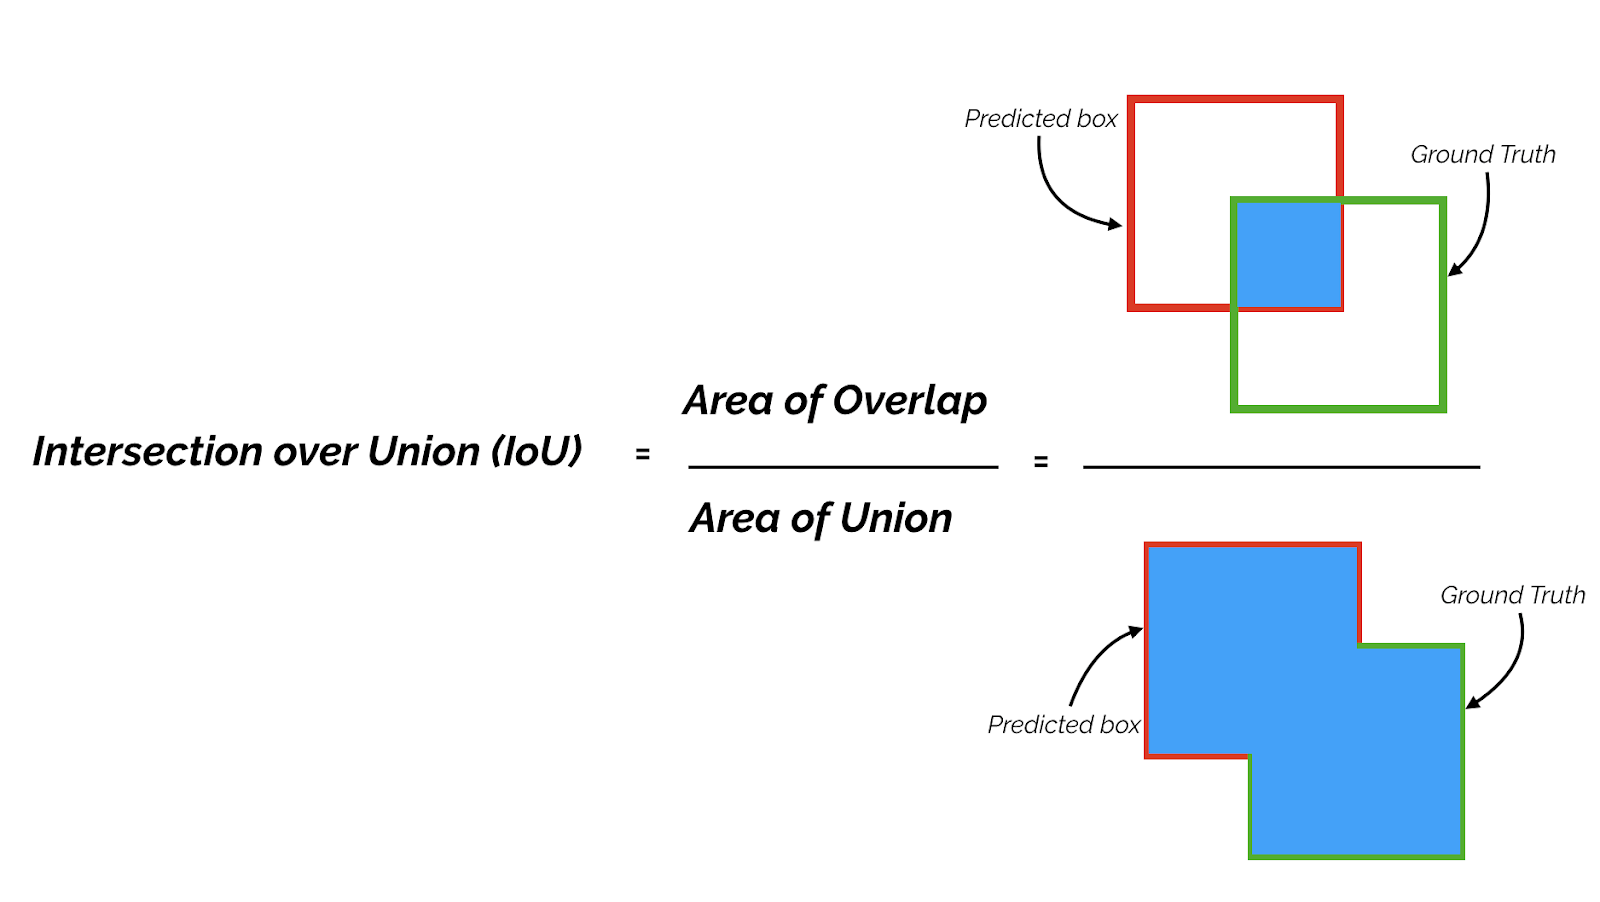
\includegraphics[width=0.45\textwidth]{img/chapters/resultados/metricas/iou.png}
\caption{\label{fig:iou}Área de superposición IoU entre los cuadros delimitadores \cite{padillaCITE2020}}
\end{figure}

\subsubsection{TP, TN, FP y FN}
\label{subsubsec:tp+tn+fp+fn}

Otros parámetros básicos en las métricas de calidad que conforman la matriz de confusión \cite{confusion-matrix} son:

\begin{itemize}
    \item \textbf{\gls{tp}}: Número de predicciones donde el clasificador predice correctamente la clase positiva como positiva. \gls{iou} $\geqslant$ \textit{threshold}
    \item \textbf{\gls{tn}}: Número de predicciones donde el clasificador predice correctamente la clase negativa como negativa. No se utiliza en el cálculo de métricas.
    \item \textbf{\gls{fp}}: Número de predicciones donde el clasificador predice incorrectamente la clase negativa como positiva. \gls{iou} <\ \textit{threshold}
    \item \textbf{\gls{fn}}: Número de predicciones donde el clasificador predice incorrectamente la clase positiva como negativa.
\end{itemize}

Típicamente el \textit{threshold} toma valores del 50\%, 75\% o 95\%.

\begin{figure}[ht]
\centering
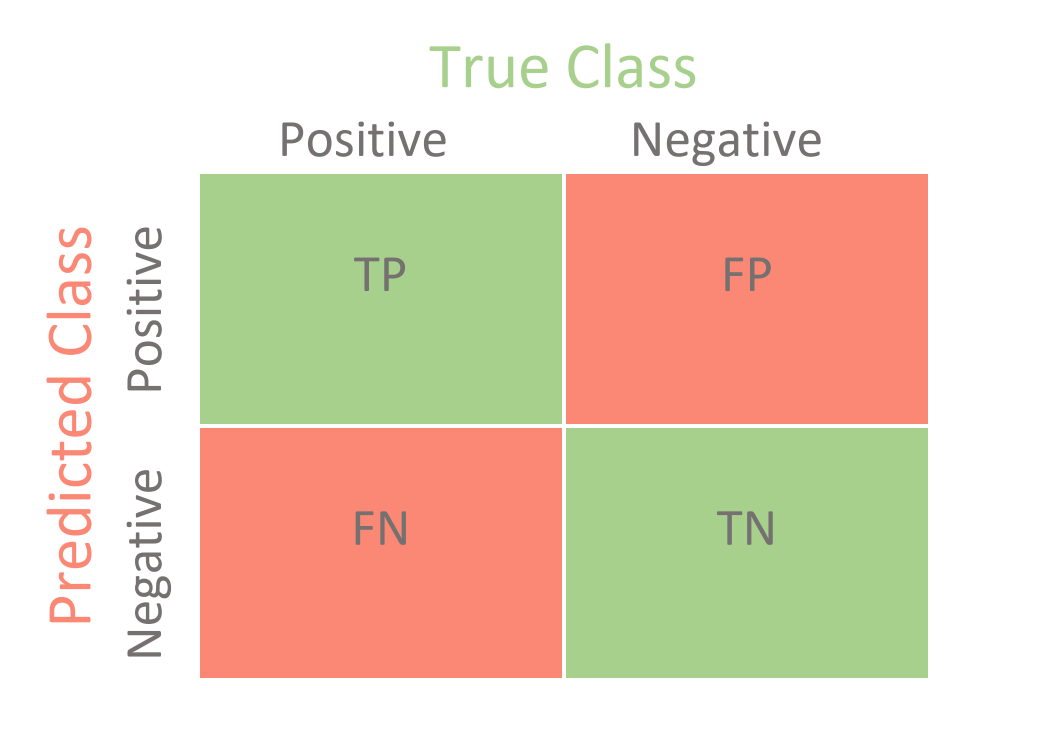
\includegraphics[width=0.45\textwidth]{img/chapters/resultados/metricas/confusion-matrix.png}
\caption{\label{fig:confusion-matrix}Matriz de confusión \cite{confusion-matrix}}
\end{figure}

\subsubsection{Precisión}
\label{subsubsec:precision}

La precisión es la capacidad de un modelo para identificar solo los objetos relevantes. Es el porcentaje de predicciones positivas correctas y viene dado por la siguiente expresión \ref{eq:precision}:

\begin{equation}
\label{eq:precision}
\text{P} = \frac{\text{TP}}{\text{TP}+\text{FP}}=\frac{\text{TP}}{\text{all detections}}
\end{equation}

\subsubsection{Recall}
\label{subsubsec:recall}

El Recall es la capacidad de un modelo para encontrar todos los casos relevantes (todos los cuadros delimitadores de ground truth). Es el porcentaje de verdadero positivo detectado entre todos los ground truths relevantes y viene dado por la siguiente expresión \ref{eq:recall}:

\begin{equation}
\label{eq:recall}
\text{R} = \frac{\text{TP}}{\text{TP}+\text{FN}}=\frac{\text{TP}}{\text{all ground truths}}
\end{equation}

\subsubsection{F-Score}
\label{subsubsec:f-score}

 El F-Score se trata de una medida estadística de precisión muy utilizada en las pruebas test de algoritmos. Es la media armónica que combina los valores de la precisión y el Recall. Viene dado por la expresión \ref{eq:f-score}:

\begin{equation}
\label{eq:f-score}
\text{F} = \frac{2 \cdotp \text{P} \cdotp \text{R}}{\text{P}+\text{R}}
\end{equation}

\subsubsection{Precisión media}
\label{subsubsec:averageprecision}

La precisión media es el valor medio de 11 puntos en la curva P-R para cada posible umbral (cada probabilidad de detección) para la misma clase (Precisión-Recall). En la ecuación \ref{eq:ap} se muestra el cálculo de la precisión media:

\begin{equation}
\label{eq:ap}
\text{AP}=\frac{1}{11} \sum_{r\in \left \{ 0, 0.1, ...,1 \right \}}\rho_{\text{interp}\left ( r \right )}
\end{equation}

con

$$\rho_{\text{interp}} = \max_{\tilde{r}:\tilde{r} \geq r} \rho\left ( \tilde{r} \right )$$

donde $\rho\left ( \tilde{r} \right )$ es la precisión medida en el Recall $\tilde{r}$

Por otro lado, el \gls{map} es la media de los \gls{ap} de todas las categorías de objetos. El \gls{map} se representa mediante la siguiente ecuación:

\begin{equation}
\label{eq:map}
\text{mAP} = \frac{1}{N} \sum_{i=1}^{N} \text{AP}_{1}
\end{equation}

\subsection{Datasets utilizados}
\label{subsec:datasets-utilizados}

A continuación, se van a describir los datasets más relevantes en la detección de objetos abandonados en los sistemas de videovigilancia así como los datasets de referencia sobre las que se validará previamente, en base a las métricas de calidad, el modelo entrenado o pre-entrenado utilizado.

En la tabla \ref{tab:datasets} se resumen los contenidos más relevantes de los datasets como son: número de secuencias, longitud media en minutos, escenario o tipos de \textit{challenges}.

Los \textit{challenges} que se consideran de interés para la detección de objetos abandonados se numeran a continuación:

\begin{itemize}
    \item I = cambios de iluminación/sombras.
    \item R = objetos alejados o pequeños.
    \item P = personas estáticas en un punto durante un período de tiempo.
    \item O = oclusiones.
    \item LR = resolución vídeo baja.
    \item RO = objetos abandonados o eliminados.
\end{itemize}

\begin{table}[ht]
\centering
\caption{Datasets utilizados en la evaluación de los algoritmos}
\label{tab:datasets}
\begin{tabular}{lcccc}
\hline
\textbf{Nombre del dataset} & \textbf{\# Secuencias} & \textbf{\begin{tabular}[c]{@{}c@{}}Longitud media\\ (min)\end{tabular}} & \textbf{Escenario} & \textbf{Challenge} \\ \hline
PETS2007                    & 28                     & 1,96                                                                    & Aeropuerto         & I, R, P, O         \\
AVSSAB2007                  & 3                      & 3,46                                                                    & Estación de metro  & I, R, P, O         \\
GBA2018                     & 8                      & 0,74                                                                    & Interior           & I, R, P, O, RO     \\
ABODA                       & 11                     & 1,90                                                                    & Interior/exterior  & I, R, P, O         \\ \hline
\end{tabular}
\end{table}

\subsubsection{PETS2007 Dataset}

El dataset \gls{pets} \cite{pets2007-dataset} está formado por secuencias que contienen tres tipos de escenarios con una complejidad ascendente: personas merodeando, robo de equipaje y equipaje desatendido/abandonado.

\paragraph*{Definición de merodear}\mbox{} \\
\label{parag:definicion-merodear}

Merodear se define como el acto donde una persona entra en escena y permanece dentro de la escena durante más de t segundos. Para los propósitos de \gls{pets}, 60 segundos.

\paragraph*{Definición de objeto desatendido}\mbox{} \\
\label{parag:definicion-desatendido-objeto}

Se utilizan tres reglas para determinar si el equipaje está atendido por parte de una persona o no:

\begin{itemize}
    \item Un equipaje es propiedad y es atendido por una persona o personas que ingresan al lugar con el equipaje hasta el punto en que el equipaje no está en contacto físico con la persona (regla contextual).
    \item En este punto, el equipaje es atendido por el propietario únicamente cuando se encuentran a una distancia de un metro del equipaje (regla espacial). Todas las distancias se miden entre los centroides del objeto en el plano del suelo (es decir, z = 0). Si una persona se encuentra a 2 metros de su equipaje, el sistema no debe activar ninguna alarma.
    \item Un equipaje está desatendido cuando el propietario está a más de 3 metros del equipaje. Si una persona cruza la línea de los 3 metros, el sistema debe usar la regla espacio-temporal el equipaje. Si el equipaje se encuentra en el rango de [2,3] metros se determina como una zona de advertencia.
\end{itemize}

\paragraph*{Definición de objeto abandonado}\mbox{} \\
\label{parag:definicion-abandono-objeto}

El abandono de una pieza de equipaje se define espacial y temporalmente. El abandono se define como:

Un bulto de equipaje que ha sido desatendido por el propietario por un período de 25 segundos consecutivos en el cual el propietario no ha vuelto a atender el equipaje, ni el equipaje ha sido atendido por una segunda persona. Si una pieza de equipaje se deja desatendida durante 25 segundos, se activa una alarma.

\paragraph*{Definición de robo de pieza de equipaje}\mbox{} \\
\label{parag:definicion-robo-pieza-equipaje}

El robo de una pieza de equipaje se define utilizando únicamente una restricción espacial. El robo se define como un artículo de equipaje movido a más de 3 metros del propietario. Se puede emitir una advertencia 2 metros del propietario.

\begin{figure}[ht]
  \centering
  \begin{subfigure}[b]{0.4\textwidth}
    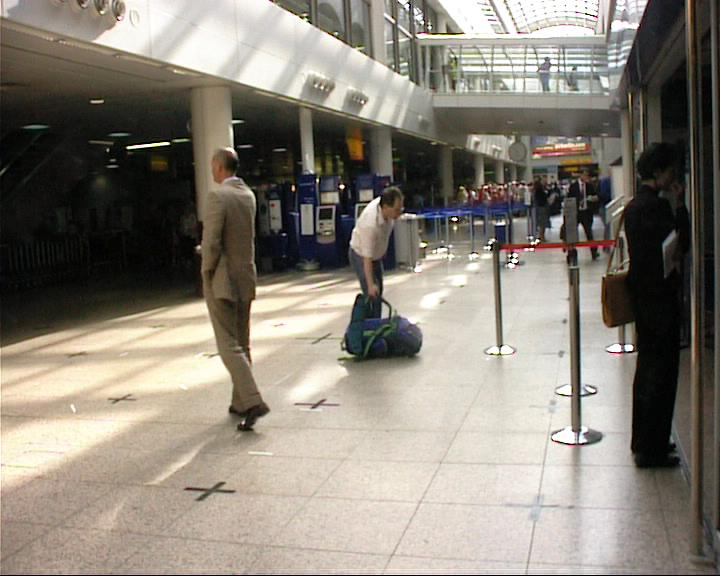
\includegraphics[width=\textwidth]{img/chapters/resultados/datasets/pets2007_1.jpg}
    \caption{}
    \label{fig:pets2007_1}
  \end{subfigure}
  \qquad\qquad
  \begin{subfigure}[b]{0.4\textwidth}
    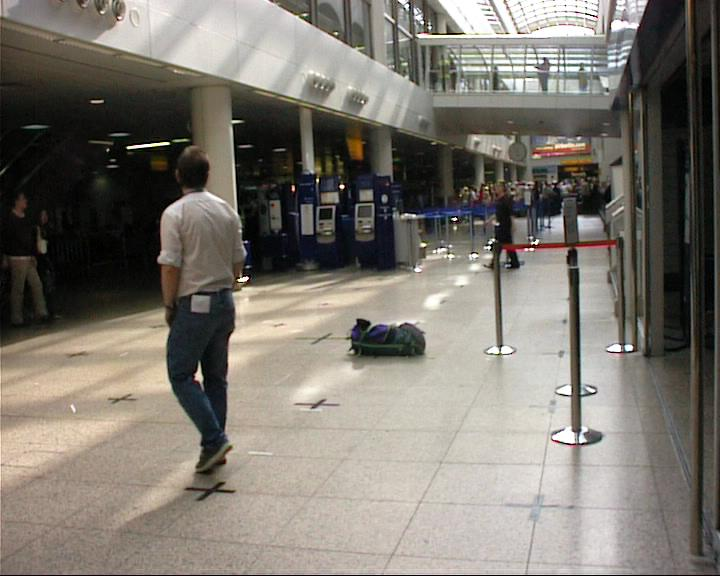
\includegraphics[width=\textwidth]{img/chapters/resultados/datasets/pets2007_2.jpg}
    \caption{}
    \label{fig:pets2007_2}
  \end{subfigure}
  \caption{Imágenes extraídas del dataset PETS2007 \cite{pets2007-dataset}.
    (\protect\subref{fig:pets2007_1}) Fotograma de la secuencia S08-camera4 donde un hombre deja su equipaje en el suelo.
    (\protect\subref{fig:pets2007_2}) Otro fotograma de la secuencia S08-camera4 donde el hombre abandona el lugar sin su equipaje.}
  \label{fig:pets2007_S08}
\end{figure}

Las cámaras utilizadas para la grabación de las distintas secuencias son las siguientes:

\begin{itemize}
    \item Cámara 1: Canon MV-1 1xCCD w/progressive scan.
    \item Cámara 2: Sony DCR-PC1000E 3xCMOS.
    \item Cámara 3: Canon MV-1 1xCCD w/progressive scan.
    \item Cámara 4: Sony DCR-PC1000E 3xCMOS.
\end{itemize}


La resolución de todas las secuencias es PAL standard (768 x 576 píxeles y 25 \gls{fps}) y comprimidas como secuencias de imágenes JPEG (aprox. 90\% de calidad).

\begin{figure}[ht]
  \centering
  \begin{subfigure}[b]{0.4\textwidth}
    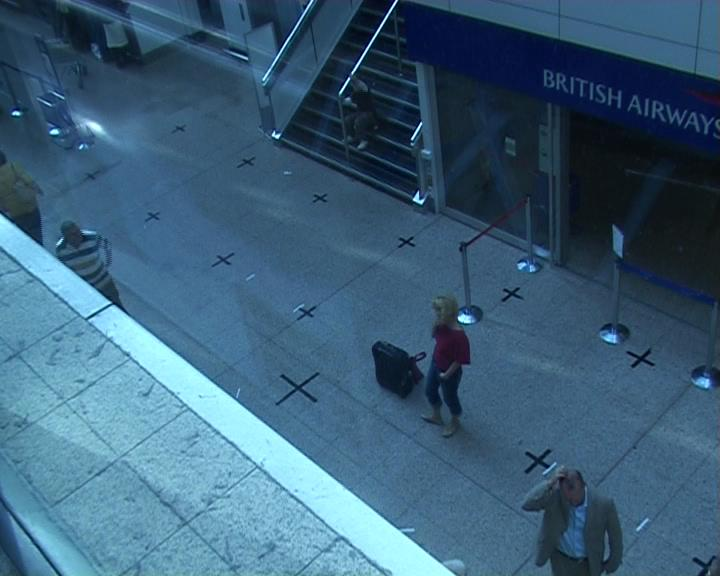
\includegraphics[width=\textwidth]{img/chapters/resultados/datasets/pets2007_3.jpg}
    \caption{}
    \label{fig:pets2007_3}
  \end{subfigure}
  \qquad\qquad
  \begin{subfigure}[b]{0.4\textwidth}
    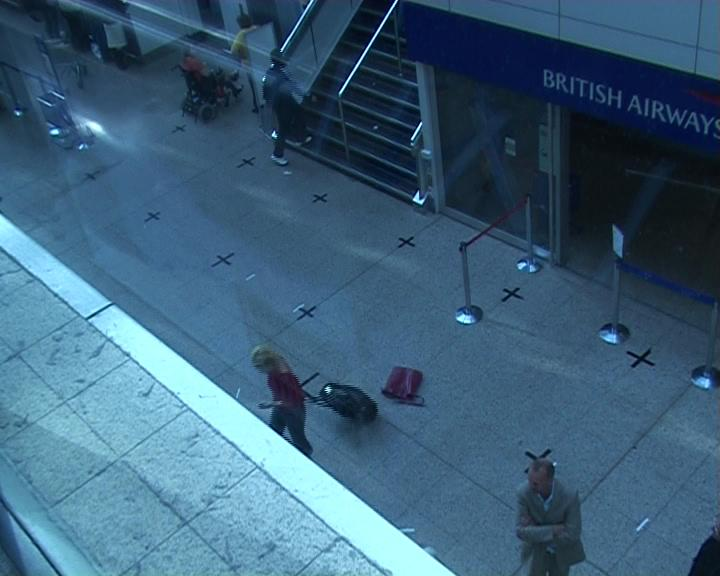
\includegraphics[width=\textwidth]{img/chapters/resultados/datasets/pets2007_4.jpg}
    \caption{}
    \label{fig:pets2007_4}
  \end{subfigure}
  \caption{Imágenes extraídas del dataset PETS2007 \cite{pets2007-dataset}.
    (\protect\subref{fig:pets2007_3}) Fotograma de la secuencia S07-thirdView donde una mujer se encuentra junto a su equipaje.
    (\protect\subref{fig:pets2007_4}) Otro fotograma de la secuencia S07-thirdView donde la mujer abandona el lugar sin su bolsa de mano.}
  \label{fig:pets2007_S07}
\end{figure}

En este proyecto solo se va a tener en cuenta cuando un equipaje ha sido abandonado sin propietario en un tiempo determinado o cuando ha sido desatendido por su propietario alejándose cierta distancia en relación a la distancia que se establece en el momento de la asociación persona-objeto.

\subsubsection{AVSSAB2007 Dataset}

\gls{avss} \cite{AVSSAB2007-dataset} es un subconjunto de datos del dataset AVSS 2007, el cual fue creado para el \textit{i-LIDS bag and vehicle detection challenge} que se celebró en la 14\textsuperscript{th} IEEE International Conference on Advanced Video and Signal based Surveillance en septiembre de 2007. En dicha conferencia se tenía como objetivo atraer artículos del Estado del Arte para presentar metodologías para la detección de eventos. Tiene la intención de informar sobre la precisión, solidez y complejidad de las secuencias de vídeo del dataset.

Se ha utilizado el subconjunto de secuencias dedicadas a la detección de objetos abandonados. Este subdataset está formado por tres secuencias de vídeo grabadas a una resolución de 720 x 576 píxeles a 25 \gls{fps}. El modelo de la cámara no se especifica.

La \gls{roi} está dividido en tres zonas: cercana, media y lejana. En cada una de las secuencias de vídeo el objeto que es abandonado se encuentra en cada una de las zonas que se muestran en la figura \ref{fig:avssab2007-zones}.

\begin{figure}[ht]
\centering
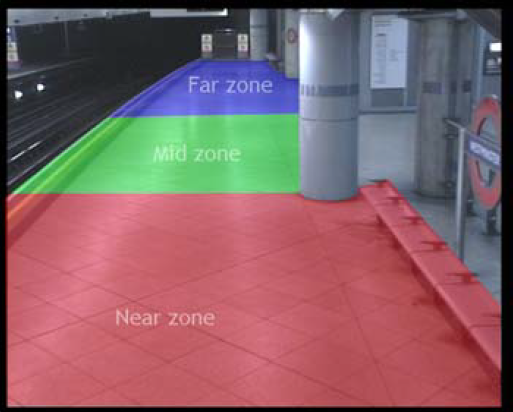
\includegraphics[width=0.4\textwidth]{img/chapters/resultados/datasets/avssab2007-zones.png}
\caption{\label{fig:avssab2007-zones}Regiones de interés del dataset AVSSAB2007 \cite{AVSSAB2007-dataset}}
\end{figure}

Todas las secuencias presentan la misma estructura en la sucesión de eventos:

\begin{itemize}
    \item Una persona ha colocado un objeto que estaba en su posesión en una de las áreas de detección.
    \item Esa persona abandona el área de detección sin el objeto.
    \item Esa persona aún no ha regresado al objeto después de 60 segundos tras haber abandonado el área de detección.
    \item El objeto permanece en el área de detección hasta finalizar la secuencia de vídeo.
\end{itemize}

\begin{figure}[ht]
  \centering
  \begin{subfigure}[b]{0.4\textwidth}
    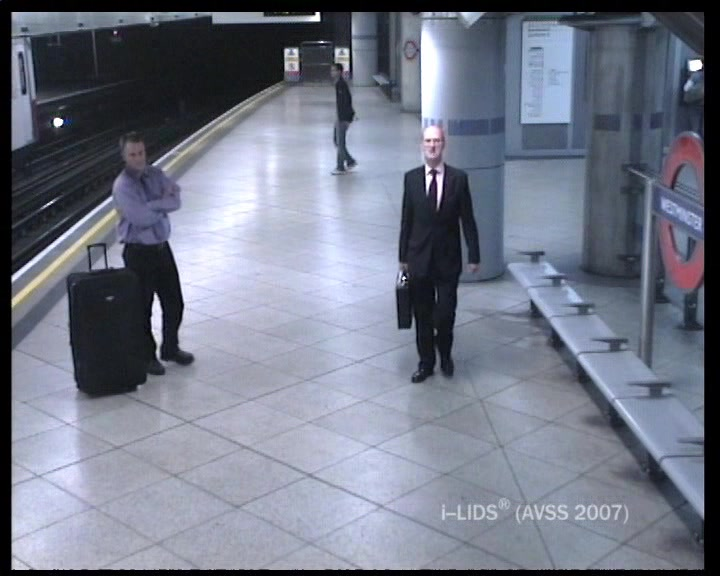
\includegraphics[width=\textwidth]{img/chapters/resultados/datasets/AVSSAB_1.jpg}
    \caption{}
    \label{fig:avssab2007_1}
  \end{subfigure}
  \qquad\qquad
  \begin{subfigure}[b]{0.4\textwidth}
    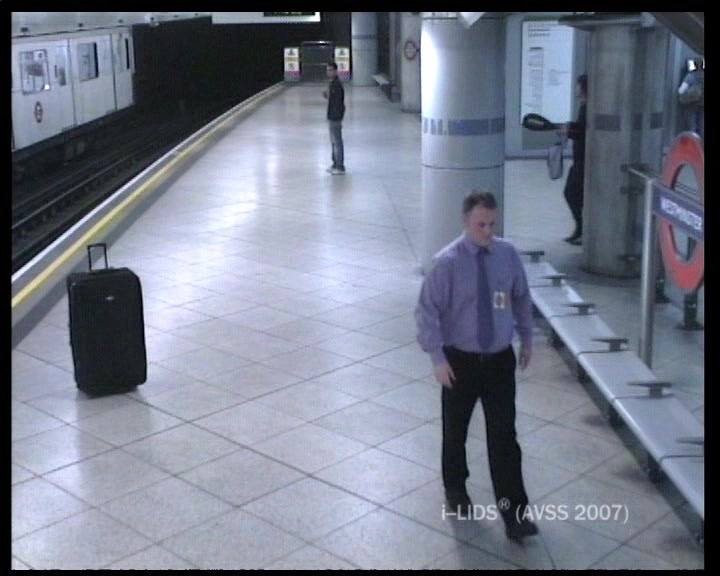
\includegraphics[width=\textwidth]{img/chapters/resultados/datasets/AVSSAB_2.jpg}
    \caption{}
    \label{fig:avssab2007_2}
  \end{subfigure}
  \caption{Imágenes extraídas del dataset AVSSAB2007 \cite{AVSSAB2007-dataset}.
    (\protect\subref{fig:avssab2007_1}) Fotograma de la secuencia AVSSAB-Easy donde el hombre abandona su maleta en la zona cercana.
    (\protect\subref{fig:avssab2007_2}) Fotograma de la secuencia AVSSAB-Medium donde una mujer se encuentra junto a su bolsa de mano en la zona media del andén del metro.}
  \label{fig:avssab2007_near_medium}
\end{figure}

\subsubsection{GBA2018 Dataset}

El dataset \gls{gba2018} \cite{gba-dataset} fue grabado y etiquetado por el grupo de investigación \gls{geintra} en la \gls{eps} de la \gls{uah} durante la realización del \gls{tfm} de David Valdivieso López \cite{valdivieso2018}. Está orientado a la evaluación de algoritmos de detección de objetos abandonados y eventos anómalos como estampidas. El dataset está formado 8 secuencias en 2 escenarios distintos grabadas con una GoPro HERO4 a una resolución de 1920 x 1080 píxeles a 60 \gls{fps}.

\begin{figure}[ht]
\centering
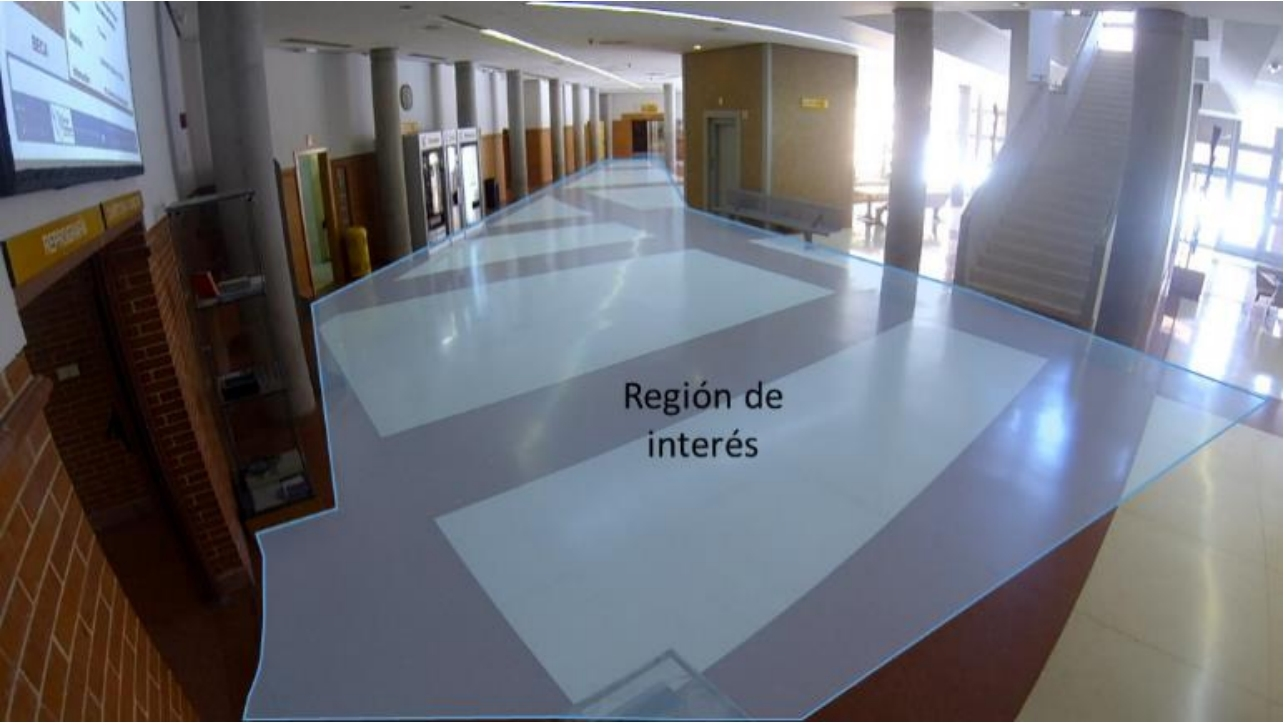
\includegraphics[width=0.4\textwidth]{img/chapters/resultados/datasets/hall-eps.jpg}
\caption{\label{fig:roi-hall-eps}ROI del hall de la Escuela Politécnica Superior (UAH) \cite{7743617}}
\end{figure}

En el primer escenario se muestra como \gls{roi} el hall de la \gls{eps} desde un plano alejado donde ocurren eventos como abandono de maletas, mochilas y bolsas de mano. Se trata de un escenario complejo ya que hay cambios tanto de luz natural como artificial y personas y objetos situados a distancias largas, lo que puede dificultar la tarea de detección.

\begin{figure}[ht!]
  \centering
  \begin{subfigure}[b]{0.4\textwidth}
    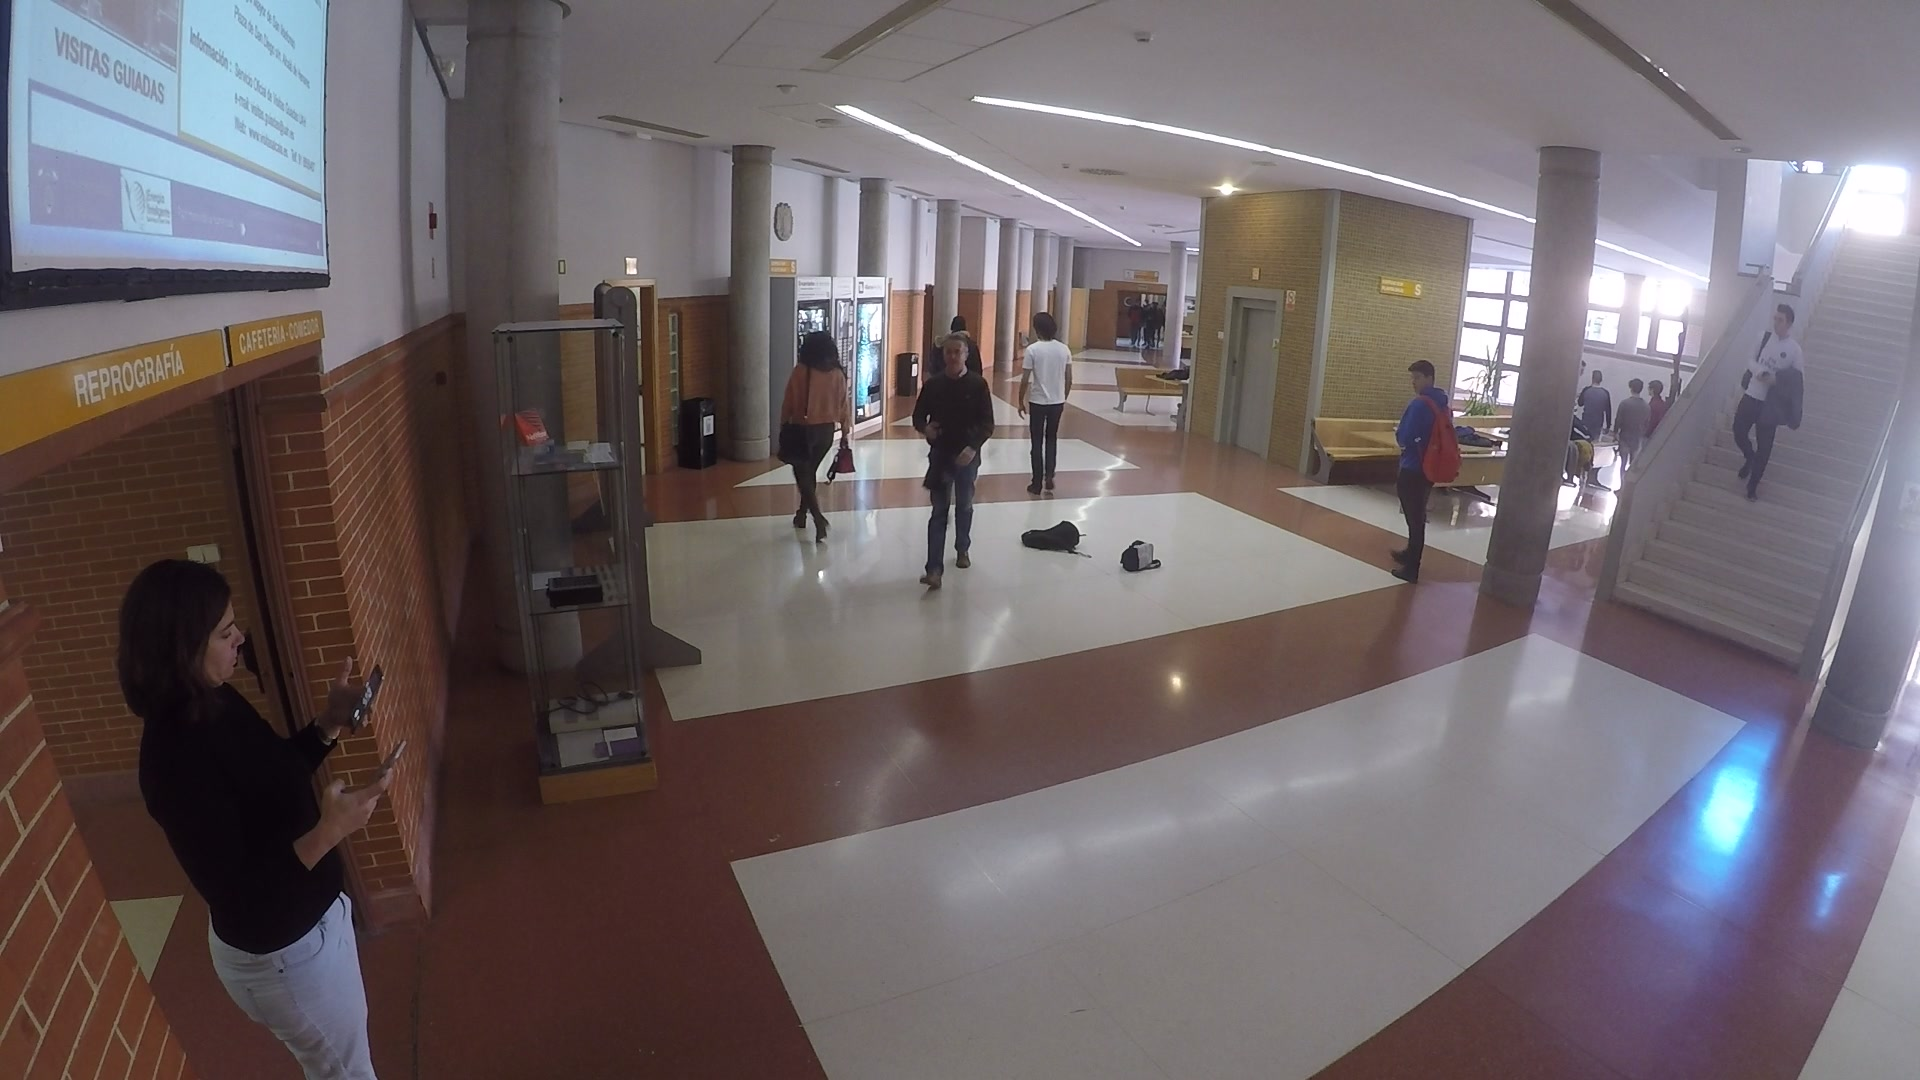
\includegraphics[width=\textwidth]{img/chapters/resultados/datasets/GBA_1.jpg}
    \caption{}
    \label{fig:GBA_1}
  \end{subfigure}
  \qquad\qquad
  \begin{subfigure}[b]{0.4\textwidth}
    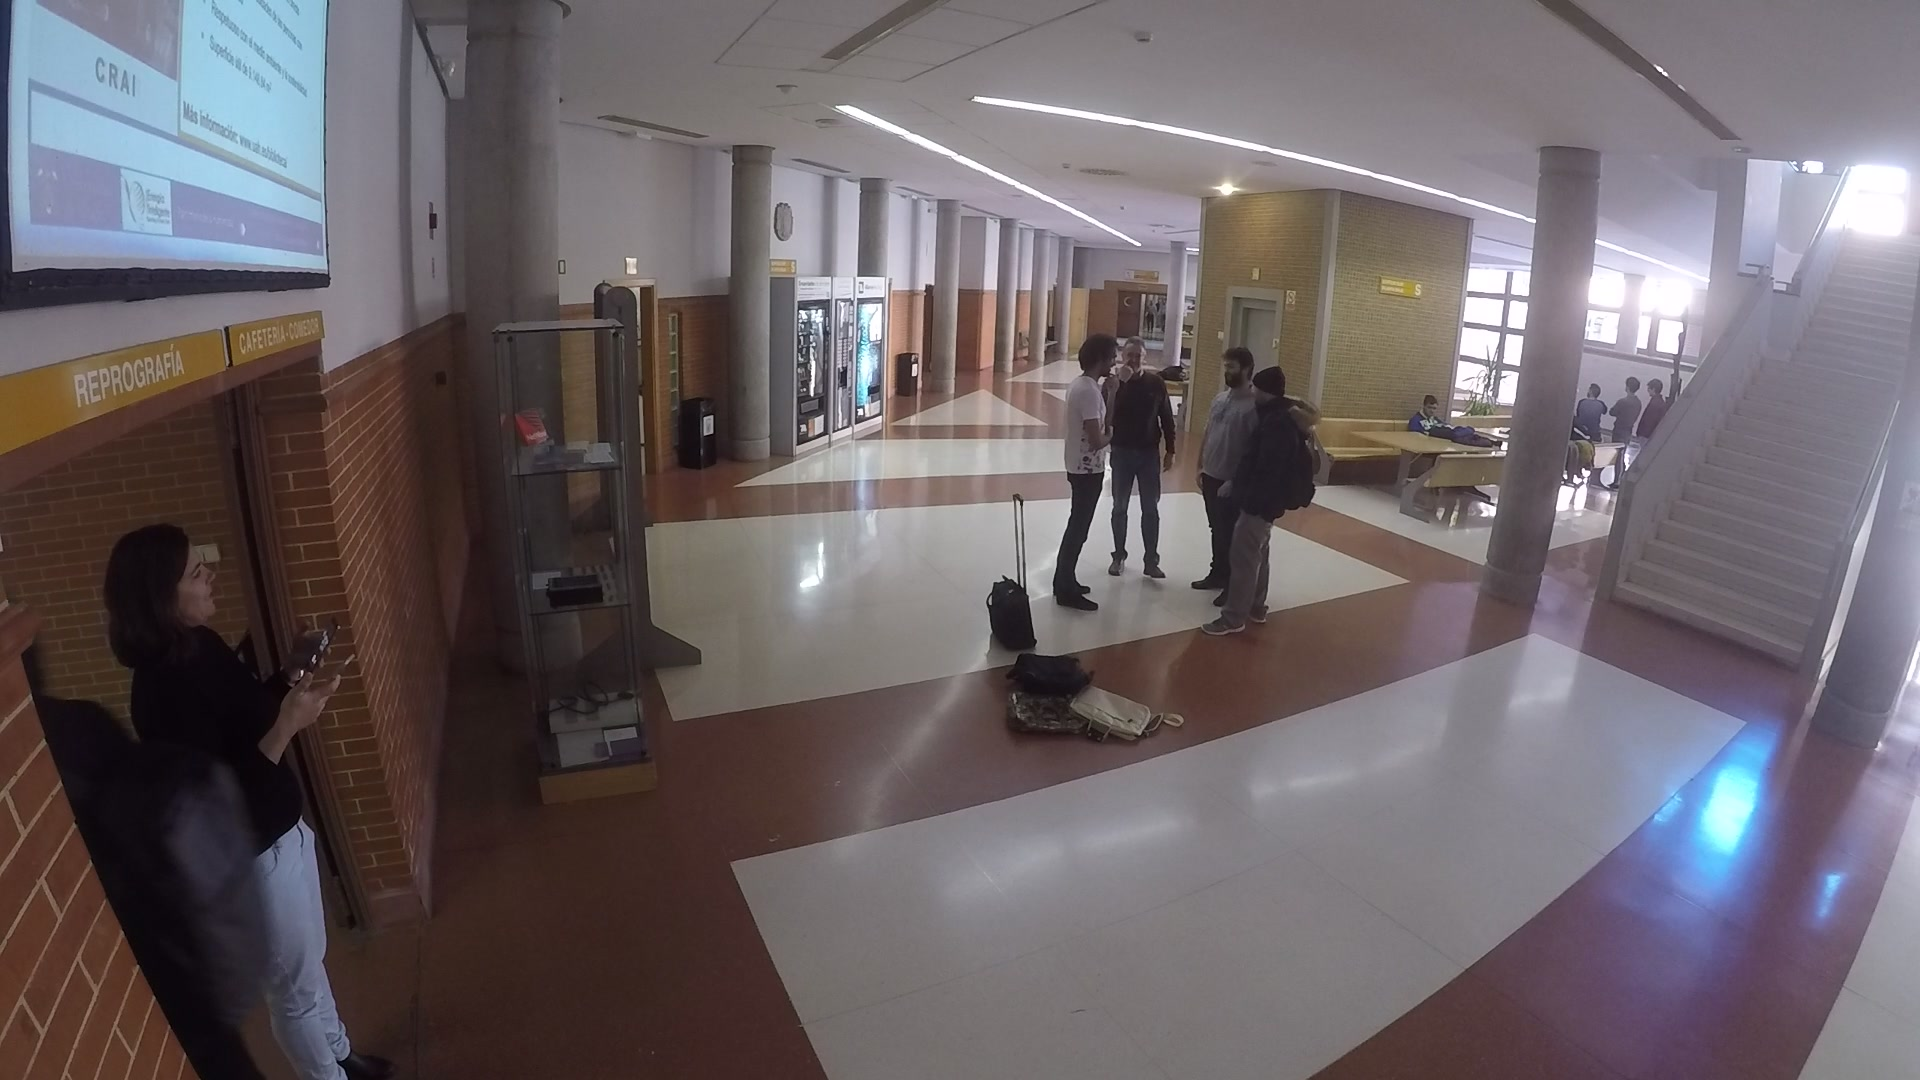
\includegraphics[width=\textwidth]{img/chapters/resultados/datasets/GBA_2.jpg}
    \caption{}
    \label{fig:GBA_2}
  \end{subfigure}
  \caption{Imágenes extraídas de secuencias del primer escenario del dataset GBA2018 \cite{gba-dataset}.
    (\protect\subref{fig:GBA_1}) Fotograma de la secuencia GBA-far-video2 donde dos bolsas de mano han sido abandonadas en medio del hall.
    (\protect\subref{fig:GBA_2}) Fotograma de la secuencia GBA-far-video3 donde varias bolsas y maletas están alejadas de sus propietarios.}
  \label{fig:GBA1}
\end{figure}

La \gls{roi} del segundo escenario se encuentra en el pasillo que conecta el hall con la cafetería. El plano de grabación es más cercano respecto al anterior por lo que se consideran secuencias más fáciles de evaluar ya que no se encuentran elementos de interés alejados ni tampoco hay cambios bruscos en la iluminación.

\begin{figure}[ht]
  \centering
  \begin{subfigure}[b]{0.4\textwidth}
    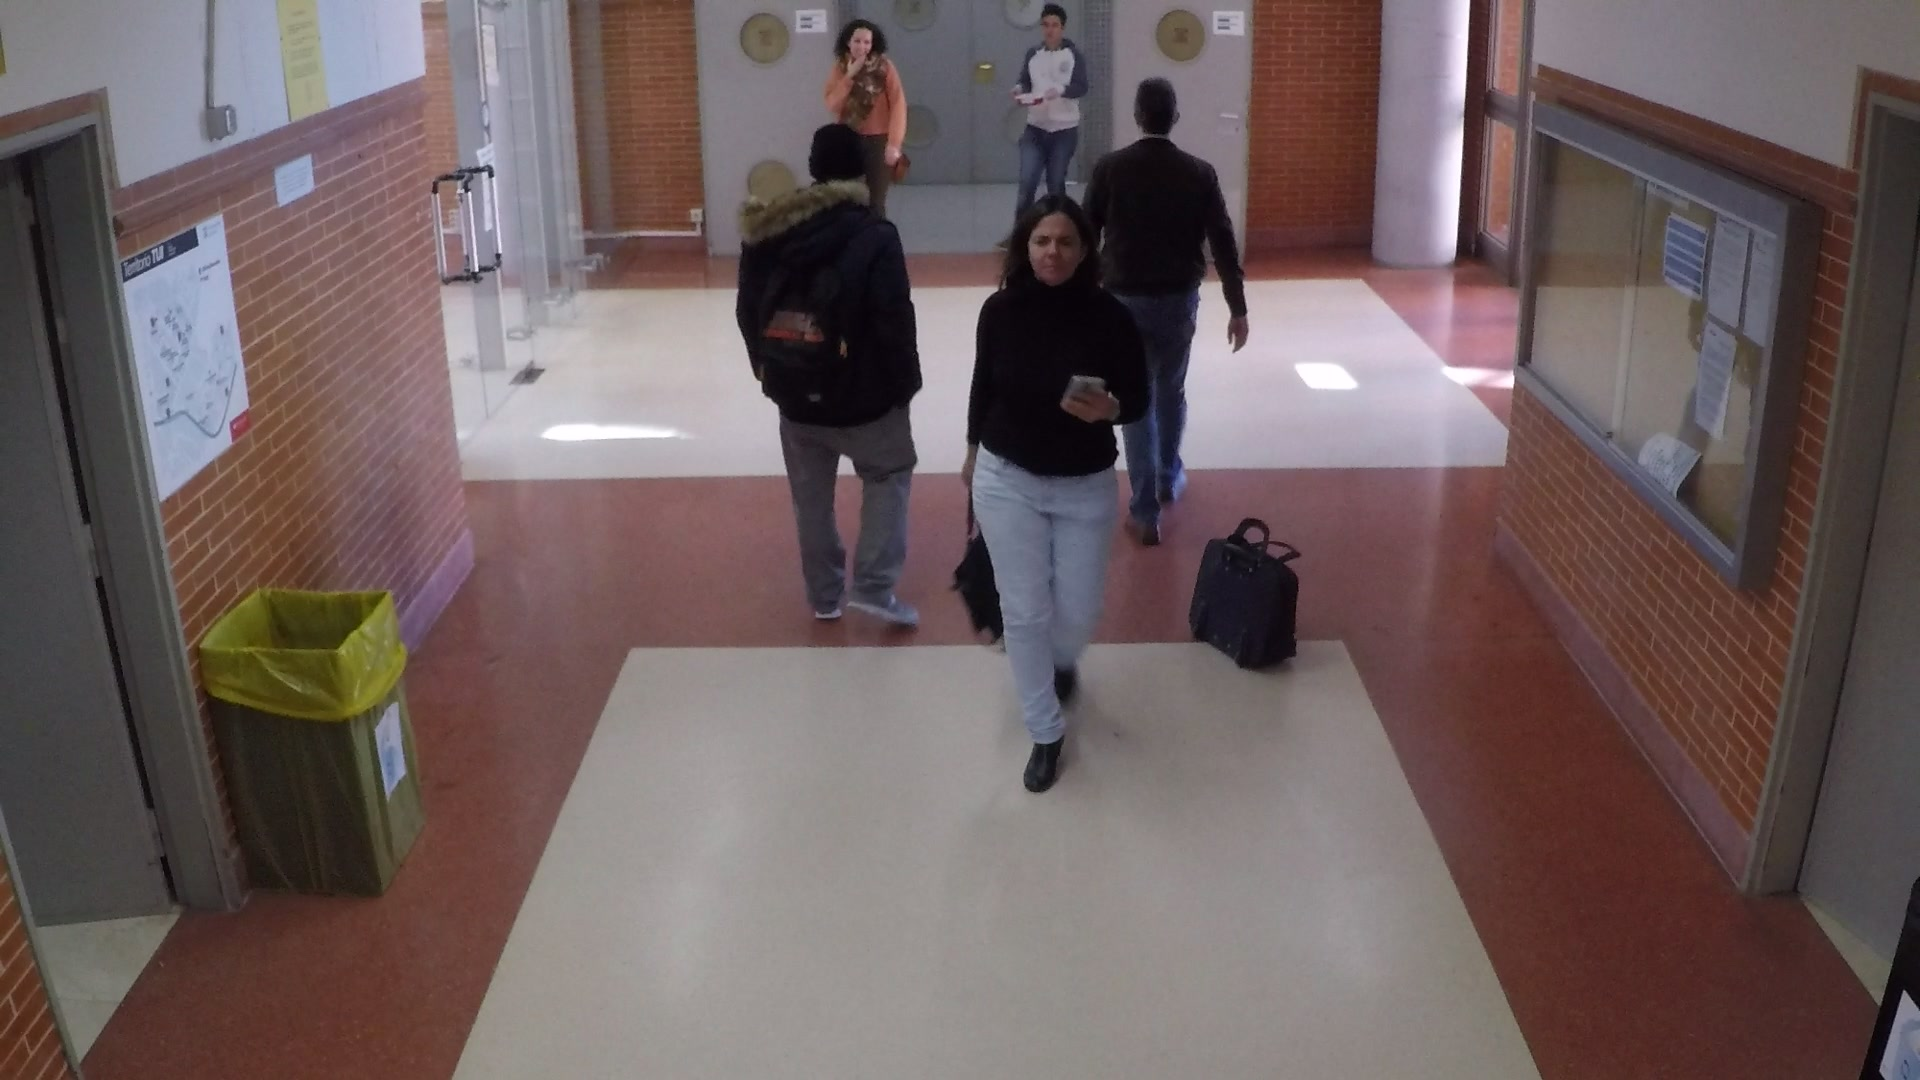
\includegraphics[width=\textwidth]{img/chapters/resultados/datasets/GBA_3.jpg}
    \caption{}
    \label{fig:GBA_3}
  \end{subfigure}
  \qquad\qquad
  \begin{subfigure}[b]{0.4\textwidth}
    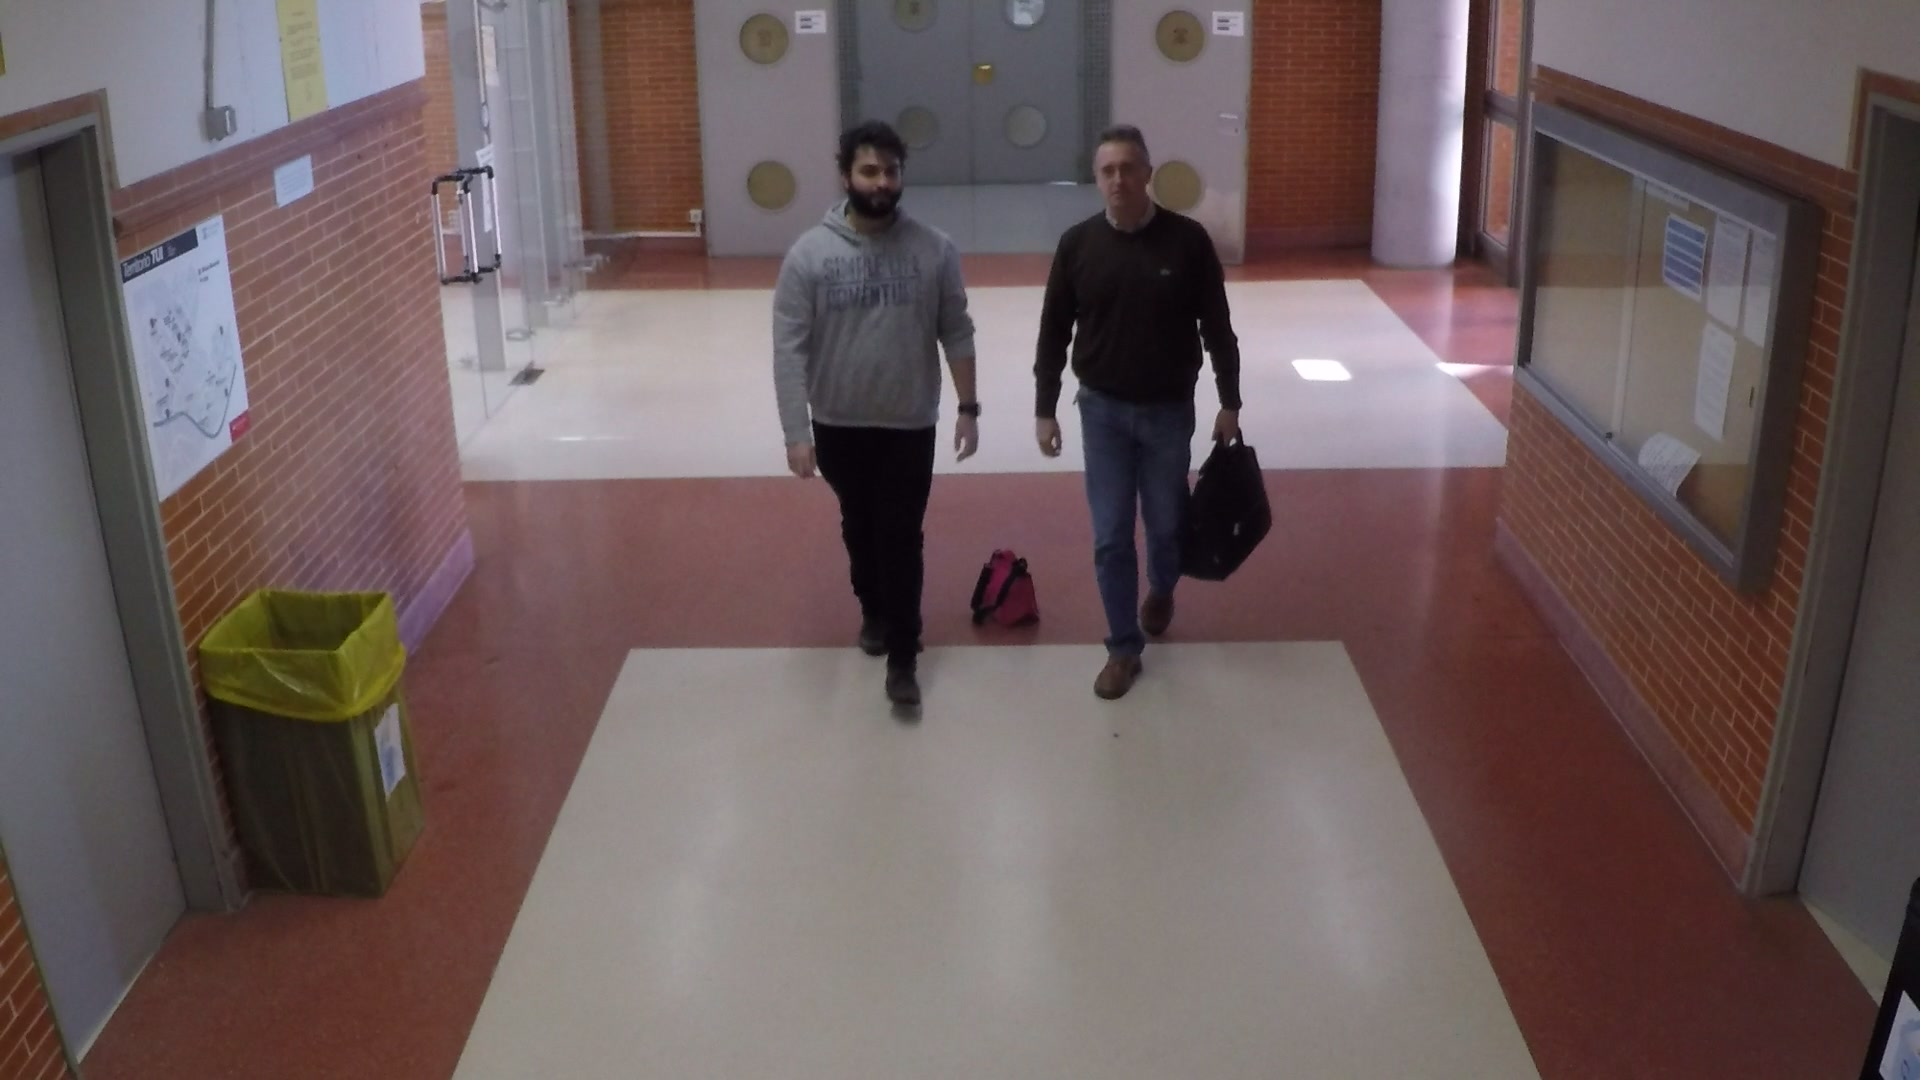
\includegraphics[width=\textwidth]{img/chapters/resultados/datasets/GBA_4.jpg}
    \caption{}
    \label{fig:GBA_4}
  \end{subfigure}
  \caption{Imágenes extraídas de secuencias del segundo escenario del dataset GBA2018 \cite{gba-dataset}.
    (\protect\subref{fig:GBA_3}) Fotograma de la secuencia GBA-near-big-video2 donde una bolsa de mano es abandonada en el pasillo de la cafetería.
    (\protect\subref{fig:GBA_4}) Fotograma de la secuencia GBA-near-big-video4 donde dos personas abandonan una pequeña bolsa de mano.}
  \label{fig:GBA2}
\end{figure}

\subsubsection{ABODA Dataset}

\gls{aboda} \cite{aboda-dataset} es un dataset propuesto por primera vez en 2015 para la detección de objetos abandonados. \gls{aboda} está formado por 11 secuencias etiquetadas con varios escenarios de aplicaciones reales, que son un desafío para la detección de objetos abandonados. Las situaciones incluyen escenas de grandes aglomeraciones de personas, cambios en las condiciones de iluminación, detección nocturna, así como ambientes interiores y exteriores.

Algunas secuencias de vídeo están grabadas a resoluciones: de 720 x 480 píxeles a 30 \gls{fps}, y otras secuencias a 640 x 480 píxeles y 30 \gls{fps}. El modelo de la cámara no se especifica.

La figura \ref{fig:aboda1} muestra los fotogramas de \texttt{video1} grabados en un entorno interior con luz artificial. En esta secuencia dos personas están interactuando entre sí y una de ellas tiene una mochila (Fig. \ref{fig:aboda_1}). Más tarde, una de las dos personas deja caer su mochila y ambos abandonan la escena ((Fig. \ref{fig:aboda_2}))

\begin{figure}[ht]
  \centering
  \begin{subfigure}[b]{0.4\textwidth}
    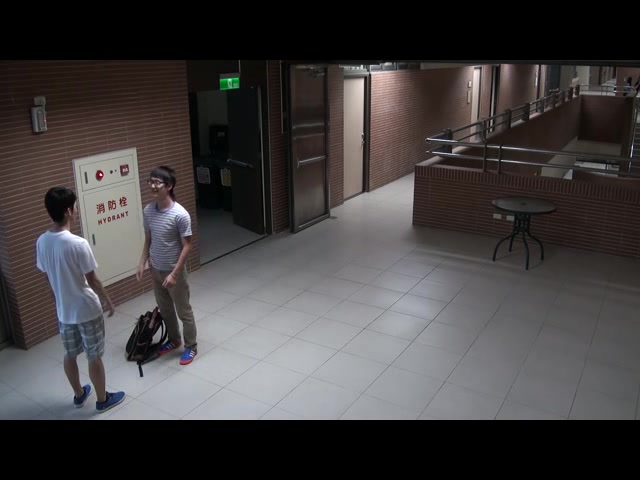
\includegraphics[width=\textwidth]{img/chapters/resultados/datasets/aboda_1.jpg}
    \caption{}
    \label{fig:aboda_1}
  \end{subfigure}
  \qquad\qquad
  \begin{subfigure}[b]{0.4\textwidth}
    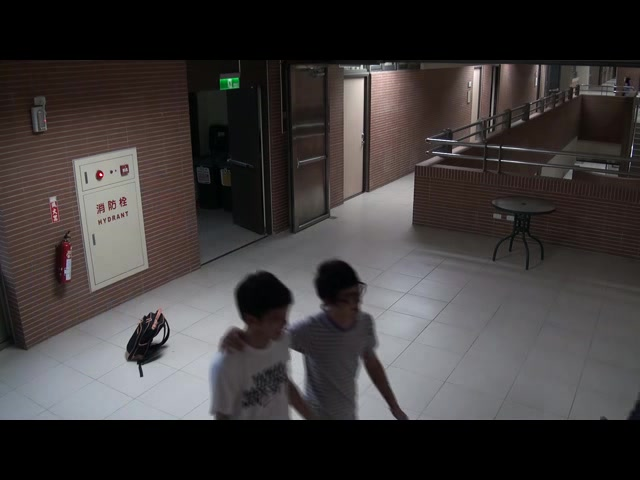
\includegraphics[width=\textwidth]{img/chapters/resultados/datasets/aboda_2.jpg}
    \caption{}
    \label{fig:aboda_2}
  \end{subfigure}
  \caption{Imágenes extraídas del dataset ABODA \cite{aboda-dataset}.
    (\protect\subref{fig:aboda_1}) Fotograma donde dos chicos conversan en el hall.
    (\protect\subref{fig:aboda_2}) Otro fotograma donde los dos chicos abandonan una mochila.}
  \label{fig:aboda1}
\end{figure}

Este dataset también incluye escenas de aglomeraciones de personas que se encuentran en aeropuertos o estaciones de tren, iluminación variable de día y grabaciones nocturnas.

\begin{figure}[ht]
  \centering
  \begin{subfigure}[b]{0.4\textwidth}
    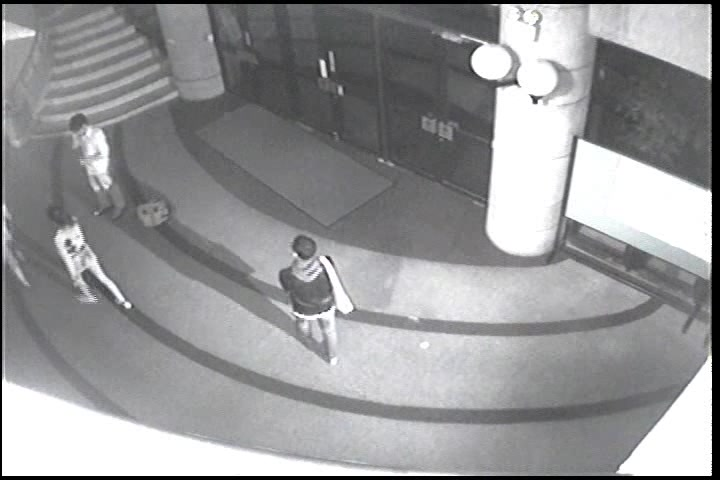
\includegraphics[width=\textwidth]{img/chapters/resultados/datasets/aboda_3.jpg}
    \caption{}
    \label{fig:aboda_3}
  \end{subfigure}
  \qquad\qquad
  \begin{subfigure}[b]{0.4\textwidth}
    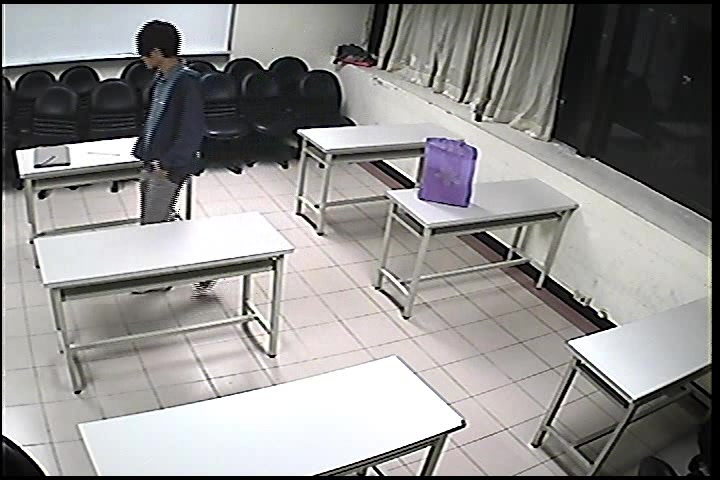
\includegraphics[width=\textwidth]{img/chapters/resultados/datasets/aboda_4.jpg}
    \caption{}
    \label{fig:aboda_4}
  \end{subfigure}
  \caption{Imágenes extraídas del dataset ABODA \cite{aboda-dataset}.
    (\protect\subref{fig:aboda_3}) Fotograma de la secuencia video5 de una grabación nocturna.
    (\protect\subref{fig:aboda_4}) Fotograma de la secuencia video11 donde hay varias personas haciendo cola en un aeropuerto.}
  \label{fig:aboda2}
\end{figure}

\section{Resultados experimentales}
\label{sec:resultados-experimentales}

Elegido \gls{coco} como dataset de referencia para entrenar y evaluar \gls{yolov4}, en las siguientes secciones se van a plasmar los resultados obtenidos en los distintos algoritmos que han sido desarrollados en el capítulo \ref{cha:desarrollo}.

Esta sección está dividida en 5 partes. Las 2 primeras partes corresponden a los resultados obtenidos en los entrenamientos de \gls{yolov4} con el dataset \gls{oidv4} que se presenció en la sección \ref{sec:train-openimagesv4}. Se realizará una evaluación cuantitativa para determinar si se toma el modelo entrenado como válido o no. Como se podrá ver a continuación, se realizaron dos entrenamientos. En el segundo entrenamiento se aumentaron el número de clases, imágenes de entrenamiento e imágenes de validación y se modificaron parámetros de la \gls{cnn} respecto al primer entrenamiento. En la 3 últimas partes, se observarán los resultados obtenidos en los 3 algoritmos desarrollados en el capítulo \ref{cha:desarrollo}, evaluando de manera cualitativa el funcionamiento de los mismos.

\subsection{Métricas de calidad en Open Image Dataset v4}
\label{subsec:metricas-calidad-openimagesv4}

En las tablas \ref{tab:metricas-test1_1}, \ref{tab:metricas-test1_2}, \ref{tab:metricas-test1_3} y \ref{tab:metricas-test1_4} se reflejan las métricas más relevantes cada 1.000 iteraciones del primer entrenamiento de la \gls{cnn} de \gls{yolov4}.

\begin{table}[ht]
\centering
\caption{Métricas de calidad en el primer entrenamiento con OIDv4 [1]}
\label{tab:metricas-test1_1}
\begin{tabular}{lcccc}
\hline
\textbf{Iterations} & \textbf{\begin{tabular}[c]{@{}c@{}}AP person\\ (\%)\end{tabular}} & \textbf{\begin{tabular}[c]{@{}c@{}}AP handbag\\ (\%)\end{tabular}} & \textbf{\begin{tabular}[c]{@{}c@{}}AP backpack\\ (\%)\end{tabular}} & \textbf{\begin{tabular}[c]{@{}c@{}}AP suitcase\\ (\%)\end{tabular}} \\ \hline
1.000               & 31,26                                                             & 85,45                                                              & 67,99                                                               & 42,15                                                               \\
\textbf{2.000}      & \textbf{43,96}                                                    & \textbf{92,39}                                                     & \textbf{63,88}                                                      & \textbf{64,79}                                                      \\
3.000               & 36,16                                                             & 90,10                                                              & 67,88                                                               & 53,33                                                               \\
4.000               & 35,56                                                             & 91,99                                                              & 64,61                                                               & 57,74                                                               \\
5.000               & 34,21                                                             & 87,35                                                              & 68,73                                                               & 48,77                                                               \\
6.000               & 36,74                                                             & 89,48                                                              & 65,83                                                               & 49,09                                                               \\
7.000               & 34,76                                                             & 88,94                                                              & 68,20                                                               & 51,24                                                               \\
8.000               & 38,30                                                             & 87,69                                                              & 72,00                                                               & 58,89                                                               \\ \hline
\end{tabular}
\end{table}

\begin{table}[ht]
\centering
\caption{Métricas de calidad en el primer entrenamiento con OIDv4 [2]}
\label{tab:metricas-test1_2}
\begin{tabular}{lcccc}
\hline
\textbf{Iterations} & \textbf{TP person} & \textbf{TP handbag} & \textbf{TP backpack} & \textbf{TP suitcase} \\ \hline
1.000               & 249                & 52                  & 19                   & 16                   \\
\textbf{2.000}      & \textbf{338}       & \textbf{54}         & \textbf{19}          & \textbf{19}          \\
3.000               & 324                & 54                  & 21                   & 18                   \\
4.000               & 329                & 54                  & 20                   & 20                   \\
5.000               & 313                & 50                  & 23                   & 16                   \\
6.000               & 323                & 52                  & 20                   & 13                   \\
7.000               & 288                & 53                  & 19                   & 18                   \\
8.000               & 308                & 49                  & 21                   & 19                   \\ \hline
\end{tabular}
\end{table}

\begin{table}[ht]
\centering
\caption{Métricas de calidad en el primer entrenamiento con OIDv4 [3]}
\label{tab:metricas-test1_3}
\begin{tabular}{lcccc}
\hline
\textbf{Iterations} & \textbf{FP person} & \textbf{FP handbag} & \textbf{FP backpack} & \textbf{FP suitcase} \\ \hline
1.000               & 416                & 20                  & 11                   & 42                   \\
\textbf{2.000}      & \textbf{489}       & \textbf{15}         & \textbf{16}          & \textbf{7}           \\
3.000               & 479                & 22                  & 18                   & 36                   \\
4.000               & 521                & 10                  & 20                   & 19                   \\
5.000               & 474                & 14                  & 19                   & 22                   \\
6.000               & 446                & 7                   & 14                   & 13                   \\
7.000               & 391                & 19                  & 13                   & 16                   \\
8.000               & 412                & 11                  & 16                   & 17                   \\ \hline
\end{tabular}
\end{table}

Como se observa en tabla \ref{tab:metricas-test1_1}, el \gls{ap} obtenido en las clases es más alto respecto a los de \gls{coco} (ver tabla \ref{tab:metricas-clases-coco}), excepto el valor obtenido en la clase \texttt{Person} que es significativamente más bajo.

En las tablas \ref{tab:metricas-test1_2} y \ref{tab:metricas-test1_3} destaca la aparición de muchos más \gls{fp} que \gls{tp} en la clase \texttt{Person}, lo que ha conducido a tener más \gls{fp} que \gls{tp} globales en todas las iteraciones (ver tabla \ref{tab:metricas-test1_4}).

En la siguiente tabla \ref{tab:metricas-test1_4} se aprecia que los mejores resultados obtenidos tuvieron lugar en la iteración 2.000, con un \textbf{44,93\%} de precisión, un \textbf{61,17\%} de Recall y un \textbf{51,81\%} de F-score. A pesar de obtener un \textbf{66,25\%} de \gls{map}, el average \gls{iou} fue del \textbf{34,13\%} debido a la alta aparición de \gls{fp} durante el entrenamiento. Se trata de un valor muy bajo.

\begin{table}[ht]
\centering
\caption{Métricas de calidad en el primer entrenamiento con OIDv4 [4]}
\label{tab:metricas-test1_4}
\begin{tabular}{lcccccccc}
\hline
\textbf{Iterations} & \textbf{TP}  & \textbf{FP}  & \textbf{FN}  & \textbf{\begin{tabular}[c]{@{}c@{}}Precision\\ (\%)\end{tabular}} & \textbf{\begin{tabular}[c]{@{}c@{}}Recall\\ (\%)\end{tabular}} & \textbf{\begin{tabular}[c]{@{}c@{}}F-score\\ (\%)\end{tabular}} & \textbf{\begin{tabular}[c]{@{}c@{}}Average IoU\\ (\%)\end{tabular}} & \textbf{\begin{tabular}[c]{@{}c@{}}mAP @ 0.5\\ (\%)\end{tabular}} \\ \hline
1.000               & 336          & 489          & 367          & 40,73                                                             & 47,80                                                          & 43,98                                                           & 29,36                                                               & 56,71                                                             \\
\textbf{2.000}      & \textbf{430} & \textbf{527} & \textbf{273} & \textbf{44,93}                                                    & \textbf{61,17}                                                 & \textbf{51,81}                                                  & \textbf{34,13}                                                      & \textbf{66,25}                                                    \\
3.000               & 417          & 555          & 286          & 42,90                                                             & 59,32                                                          & 49,79                                                           & 32,29                                                               & 61,87                                                             \\
4.000               & 423          & 570          & 280          & 42,60                                                             & 60,17                                                          & 49,88                                                           & 33,30                                                               & 62,47                                                             \\
5.000               & 402          & 529          & 301          & 43,18                                                             & 57,18                                                          & 49,20                                                           & 32,53                                                               & 59,77                                                             \\
6.000               & 408          & 480          & 295          & 45,95                                                             & 58,04                                                          & 51,29                                                           & 36,76                                                               & 60,28                                                             \\
7.000               & 378          & 439          & 325          & 46,27                                                             & 53,77                                                          & 49,74                                                           & 36,90                                                               & 60,78                                                             \\
8.000               & 397          & 456          & 306          & 46,54                                                             & 56,47                                                          & 51,03                                                           & 37,69                                                               & 64,22                                                             \\ \hline
\end{tabular}
\end{table}

En la figura \ref{fig:metrics-train1} se ilustra la evolución de las métricas en función de las iteraciones transcurridas. Estableciendo como métrica de prioridad el \gls{map}, los mejores resultados se obtuvieron en la iteración 2.000. A partir de este punto oscilaron levemente con tendencia decreciente.

\begin{figure}[ht]
\centering
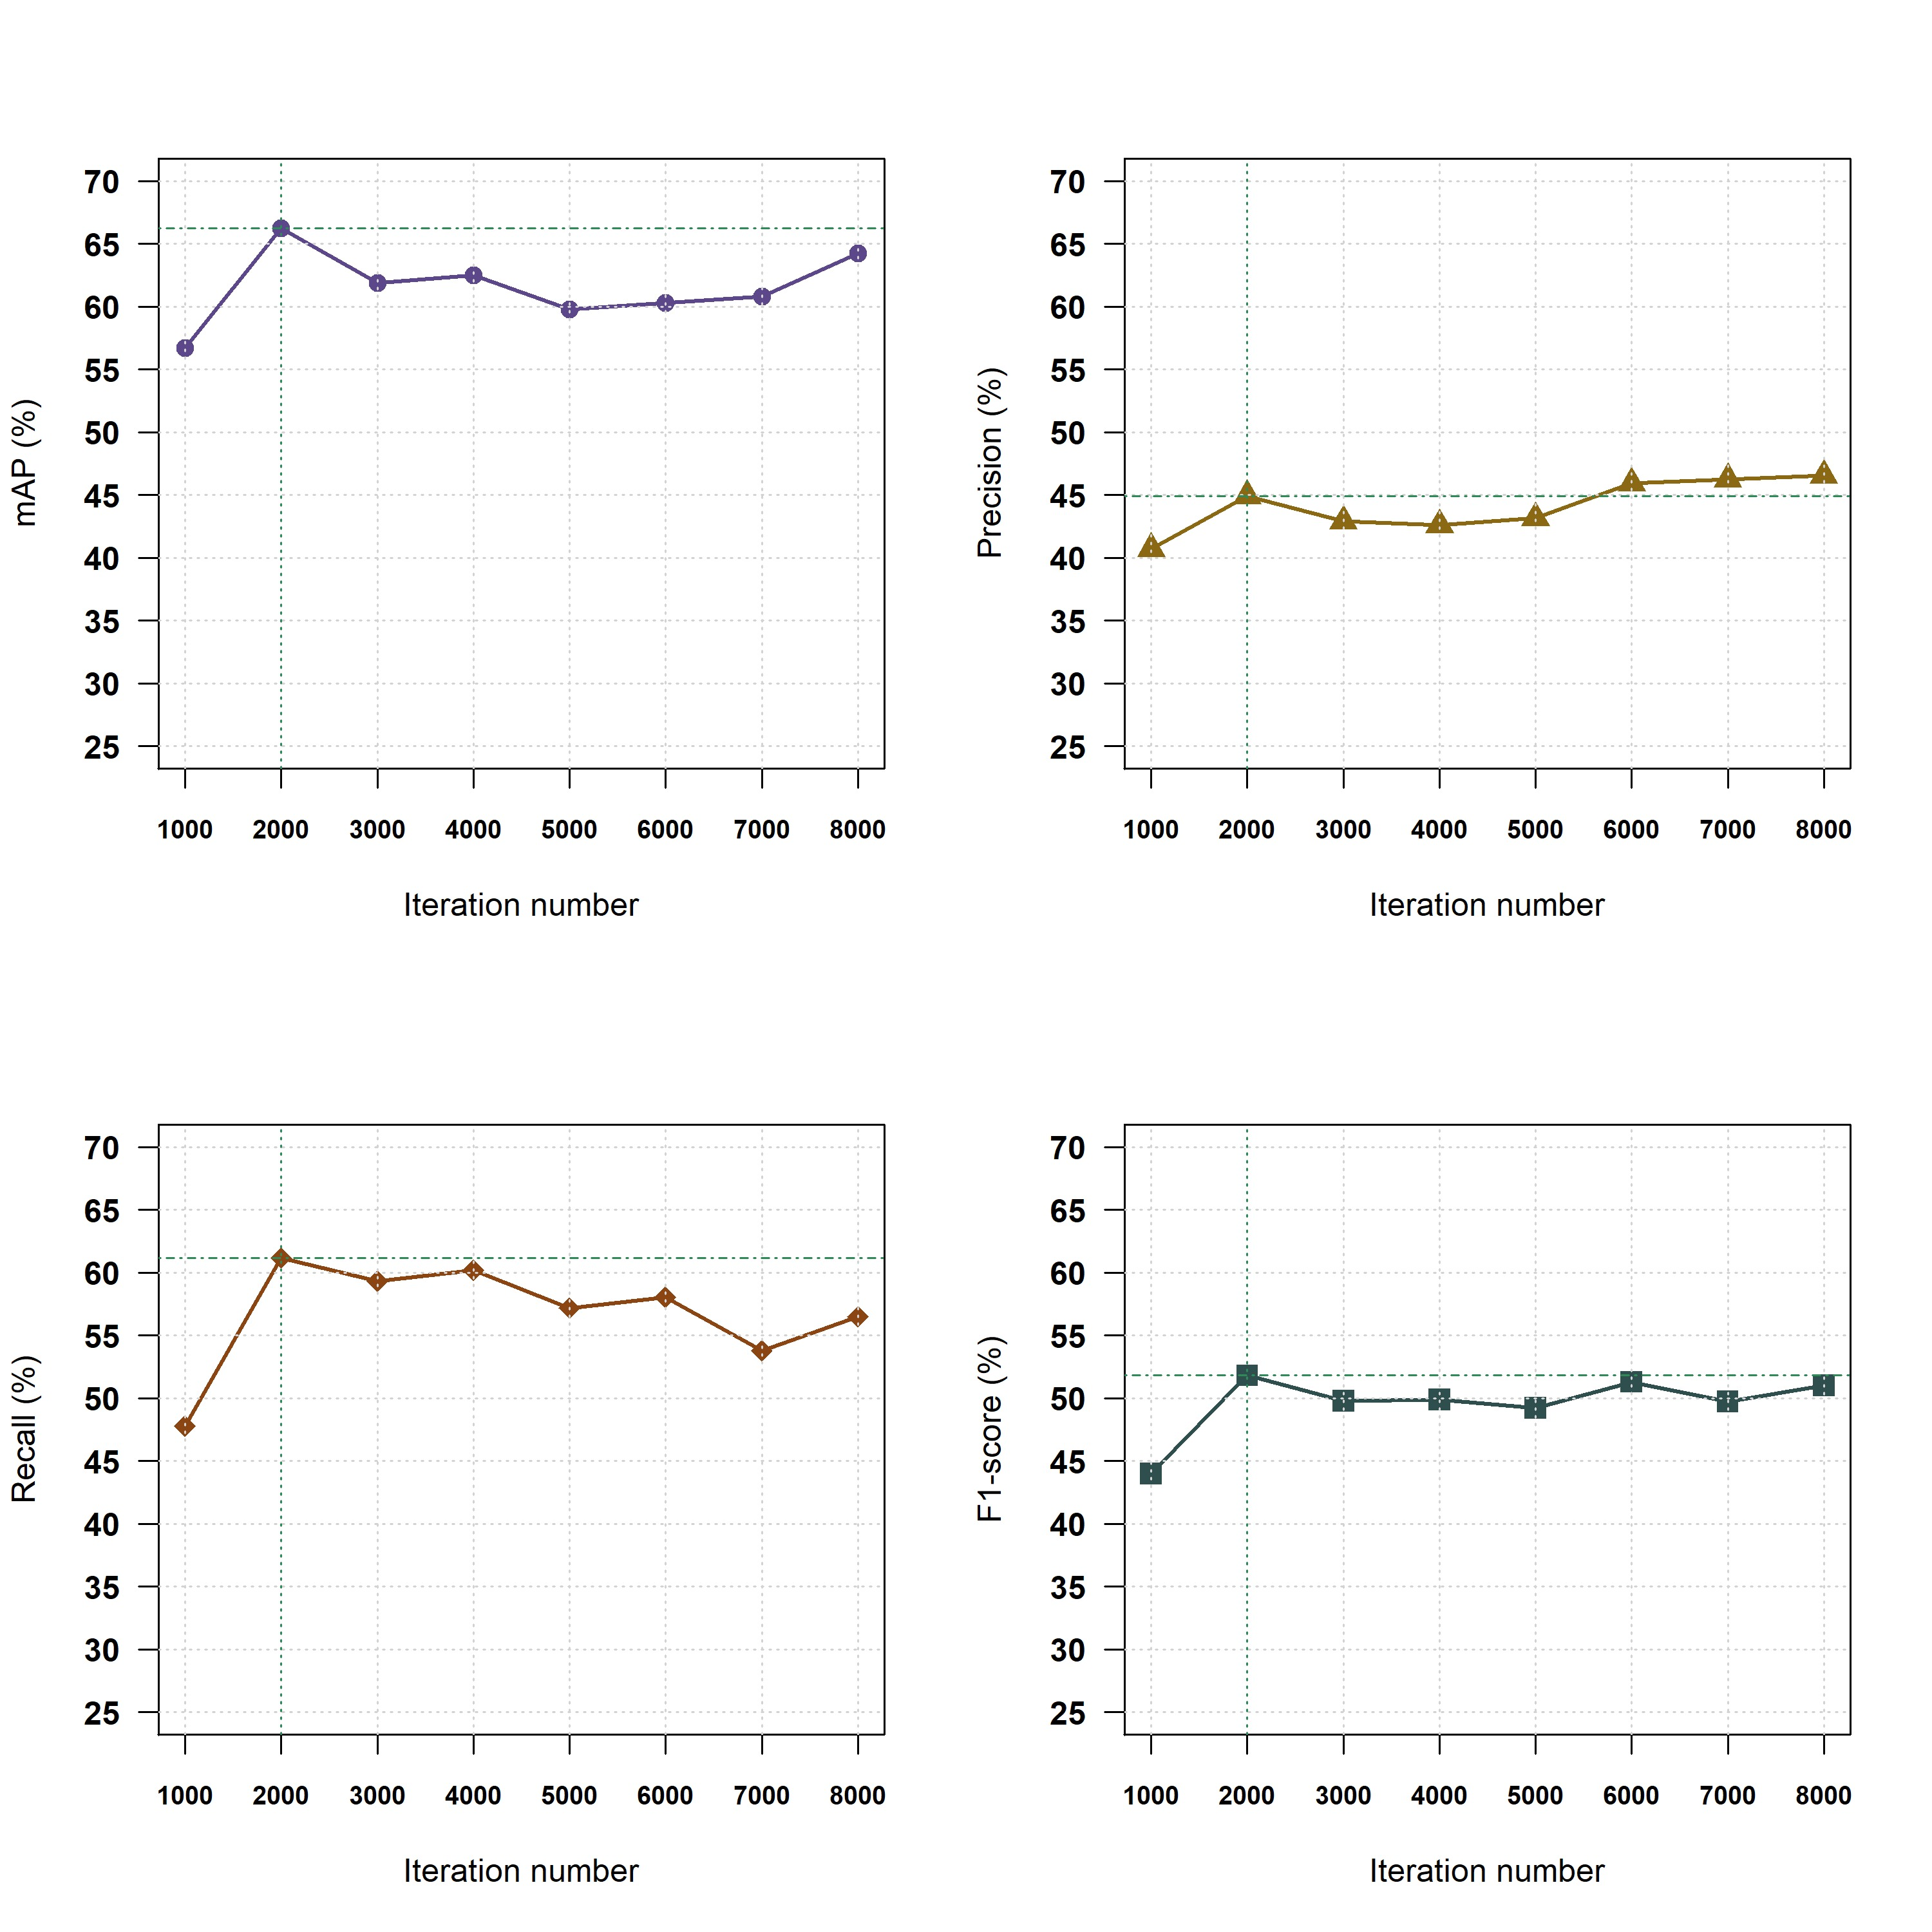
\includegraphics[width=0.67\textwidth]{img/chapters/resultados/metricas/metrics-train1.png}
\caption{\label{fig:metrics-train1}Resumen métricas primer entrenamiento de la red neuronal con el dataset de OIDv4}
\end{figure}

Como se ha podido observar, los resultados obtenidos no han sido favorables. A pesar de tener un \gls{map} superior al de \gls{coco}, el average \gls{iou} es significativamente más bajo que el \textbf{56,04\%} de \gls{coco} (ver tabla \ref{tab:comparativa-metricas2}).

Por ello, se ha realizado un nuevo entrenamiento modificando algunos parámetros de la \gls{cnn} y aumentando el número de clases y de imágenes de entrenamiento y validación. El dataset \gls{oidv4} dispone de clases más especificas de equipajes o bolsas de mano que \gls{coco}.

Se ha realizado el mismo procedimiento que se hizo en la sección \ref{sec:train-openimagesv4}, añadiendo las clases de interés: \texttt{`Plastic bag', `Luggage and bags'} y \texttt{`Briefcase'}. Estas 3 nuevas clases posteriormente se han unificado junto a las anteriores como una única clase llamada \texttt{`bags'}. Se han aumentado el valor de las variables de redimensionamiento de imágenes a la entrada de la red \texttt{width} y \texttt{height} a 608 para garantizar una mayor precisión a costa de un mayor tiempo de entrenamiento. El número de imágenes de entrenamiento se ha subido a 3.000 y las de validación a 600 en la clase \texttt{Person}.

El número máximo de iteraciones (\texttt{max\_batches}) se ha fijado a 20.000 iteraciones. A pesar de que lo recomendable es fijarlo a (\# de clases) * 2.000, se ha aumentado para analizar en un mayor número de iteraciones la evolución de los valores de las métricas. El resto de parámetros de configuración de la red \gls{yolov4} se han adaptado al nuevo número de clases a entrenar, del mismo modo que se realizó en la sección \ref{subsec:configuracion-ficheros-training}.

En las tablas  \ref{tab:metricas-test2_1} y \ref{tab:metricas-test2_2} se reflejan las métricas más relevantes cada 1.000 iteraciones del segundo entrenamiento de la \gls{cnn} de \gls{yolov4}.

\begin{table}[ht]
\centering
\caption{Métricas de calidad en el segundo entrenamiento con OIDv4 [1]}
\label{tab:metricas-test2_1}
\begin{tabular}{lcccccc}
\hline
\textbf{Iterations} & \textbf{\begin{tabular}[c]{@{}c@{}}AP person\\ (\%)\end{tabular}} & \textbf{\begin{tabular}[c]{@{}c@{}}AP bags\\ (\%)\end{tabular}} & \textbf{TP person} & \textbf{TP bags} & \textbf{FP person} & \textbf{FP bags} \\ \hline
1.000               & 30,81                                                             & 21,61                                                           & 5.216              & 231               & 9.220              & 579              \\
2.000               & 38,38                                                             & 53,59                                                           & 6.542              & 362               & 11.789             & 354              \\
3.000               & 33,51                                                             & 68,56                                                           & 7.232              & 419               & 18.887             & 411              \\
4.000               & 41,31                                                             & 77,12                                                           & 7.105              & 427               & 11.397             & 222              \\
5.000               & 38,86                                                             & 75,78                                                           & 6.586              & 444               & 11.735             & 398              \\
6.000               & 36,29                                                             & 66,49                                                           & 6.556              & 426               & 12.506             & 537              \\
7.000               & 39,94                                                             & 67,78                                                           & 6.246              & 418               & 9.744              & 523              \\
8.000               & 31,69                                                             & 69,07                                                           & 6.082              & 417               & 13.353             & 422              \\
9.000               & 43,34                                                             & 78,37                                                           & 6.773              & 451               & 9.846              & 373              \\
\textbf{10.000}     & \textbf{43,40}                                                    & \textbf{78,53}                                                  & \textbf{6.174}     & \textbf{426}      & \textbf{7.149}     & \textbf{217}     \\
11.000              & 38,81                                                             & 76,60                                                           & 7.166              & 446               & 12.162             & 387              \\
12.000              & 41,72                                                             & 78,10                                                           & 6.926              & 444               & 10.387             & 289              \\
13.000              & 39,48                                                             & 74,67                                                           & 6.575              & 406               & 9.850              & 238              \\
14.000              & 41,85                                                             & 73,69                                                           & 6.844              & 432               & 10.092             & 385              \\
15.000              & 40,19                                                             & 75,37                                                           & 6.915              & 423               & 11.426             & 252              \\
16.000              & 41,26                                                             & 75,17                                                           & 6.661              & 423               & 9.330              & 219              \\
17.000              & 42,13                                                             & 78,77                                                           & 6.991              & 433               & 9.924              & 242              \\
18.000              & 40,97                                                             & 75,45                                                           & 6.871              & 432               & 10.243             & 300              \\
19.000              & 39,01                                                             & 73,23                                                           & 6.822              & 428               & 10.791             & 333              \\
20.000              & 41,37                                                             & 78,38                                                           & 7.011              & 432               & 10.103             & 232              \\ \hline
\end{tabular}
\end{table}

\begin{table}[ht!]
\centering
\caption{Métricas de calidad en el segundo entrenamiento con OIDv4 [2]}
\label{tab:metricas-test2_2}
\begin{tabular}{lcccccccc}
\hline
\textbf{Iterations} & \textbf{TP}    & \textbf{FP}    & \textbf{FN}    & \textbf{\begin{tabular}[c]{@{}c@{}}Precision\\ (\%)\end{tabular}} & \textbf{\begin{tabular}[c]{@{}c@{}}Recall\\ (\%)\end{tabular}} & \textbf{\begin{tabular}[c]{@{}c@{}}F-score\\ (\%)\end{tabular}} & \textbf{\begin{tabular}[c]{@{}c@{}}Average\\ IoU (\%)\end{tabular}} & \textbf{\begin{tabular}[c]{@{}c@{}}mAP @ 0.5\\ (\%)\end{tabular}} \\ \hline
1.000               & 5.447          & 9.799          & 6.379          & 35,73                                                             & 46,06                                                          & 40,24                                                           & 25,72                                                               & 26,21                                                             \\
2.000               & 6.904          & 12.143         & 4.922          & 36,25                                                             & 58,38                                                          & 44,73                                                           & 27,30                                                               & 45,98                                                             \\
3.000               & 7.651          & 19.298         & 4.175          & 28,39                                                             & 64,70                                                          & 39,46                                                           & 21,66                                                               & 51,04                                                             \\
4.000               & 7.532          & 11.619         & 4.294          & 39,33                                                             & 63,69                                                          & 48,63                                                           & 30,90                                                               & 59,22                                                             \\
5.000               & 7.030          & 12.133         & 4.796          & 36,69                                                             & 59,45                                                          & 45,37                                                           & 28,28                                                               & 57,32                                                             \\
6.000               & 6.982          & 13.043         & 4.844          & 34,87                                                             & 59,04                                                          & 43,84                                                           & 27,23                                                               & 51,39                                                             \\
7.000               & 6.664          & 10.267         & 5.162          & 39,36                                                             & 56,35                                                          & 46,35                                                           & 30,96                                                               & 53,86                                                             \\
8.000               & 6.499          & 13.775         & 5.327          & 32,06                                                             & 54,96                                                          & 40,49                                                           & 24,96                                                               & 50,38                                                             \\
9.000               & 7.224          & 10.219         & 4.602          & 41,41                                                             & 61,09                                                          & 49,36                                                           & 32,95                                                               & 60,85                                                             \\
\textbf{10.000}     & \textbf{6.600} & \textbf{7.366} & \textbf{5.226} & \textbf{47,26}                                                    & \textbf{55,81}                                                 & \textbf{51,18}                                                  & \textbf{37,83}                                                      & \textbf{60,97}                                                    \\
11.000              & 7.612          & 12.549         & 4.214          & 37,76                                                             & 64,37                                                          & 47,59                                                           & 30,20                                                               & 57,70                                                             \\
12.000              & 7.370          & 10.676         & 4.456          & 40,84                                                             & 62,32                                                          & 49,34                                                           & 32,34                                                               & 59,91                                                             \\
13.000              & 6.981          & 10.088         & 4.845          & 40,90                                                             & 59,03                                                          & 48,32                                                           & 32,83                                                               & 57,07                                                             \\
14.000              & 7.276          & 10.477         & 4.550          & 40,98                                                             & 61,53                                                          & 49,20                                                           & 32,61                                                               & 57,77                                                             \\
15.000              & 7.338          & 11.678         & 4.488          & 38,59                                                             & 62,05                                                          & 47,58                                                           & 30,53                                                               & 57,78                                                             \\
16.000              & 7.084          & 9.549          & 4.742          & 42,59                                                             & 59,90                                                          & 49,78                                                           & 33,87                                                               & 58,22                                                             \\
17.000              & 7.424          & 10.166         & 4.402          & 42,21                                                             & 62,78                                                          & 50,48                                                           & 34,53                                                               & 60,45                                                             \\
18.000              & 7.303          & 10.543         & 4.523          & 40,92                                                             & 61,75                                                          & 49,22                                                           & 33,11                                                               & 58,21                                                             \\
19.000              & 7.250          & 11.124         & 4.576          & 39,46                                                             & 61,31                                                          & 48,01                                                           & 31,90                                                               & 56,12                                                             \\
20.000              & 7.443          & 10.335         & 4.383          & 41,87                                                             & 62,94                                                          & 50,28                                                           & 34,35                                                               & 59,93                                                             \\ \hline
\end{tabular}
\end{table}

De nuevo, no se han obtenido los resultados esperados. En la tabla \ref{tab:metricas-test2_1} se observa un valor de \gls{ap} de la clase \texttt{Person} inferior al conseguido en \gls{coco} (ver tabla \ref{tab:metricas-clases-coco}) a pesar de aumentar al doble el número de imágenes en el entrenamiento. El conjunto de todas las clases de interés \texttt{bags} representan un valor alto de \gls{ap} y una vez más, la cantidad de \gls{fp} es mayor a los \gls{tp} debido a la clase \texttt{Person}. Esto deriva a obtener un average \gls{iou} más bajo del esperado a pesar de obtener valores aceptables en precición, Recall, F-score y \gls{map}.

Los resultados obtenidos son muy similares a los del primer entrenamiento pese a modificar parámetros de configuración del fichero \texttt{yolov4-obj.cfg}, aumentar el número de clases de los objetos de interés y aumentar el número de imágenes de entrenamiento y validación de la clase \texttt{Person}, clase que obtuvo malos resultados en el primer entrenamiento.

En la tabla \ref{tab:metricas-test2_2} se aprecia que los mejores resultados obtenidos tuvieron lugar en la iteración 10.000, con un \textbf{47,26\%} de precisión, un \textbf{55,81\%} de Recall y un \textbf{51,18\%} de F-score. A pesar de obtener un \textbf{60,97\%} de \gls{map}, el average \gls{iou} fue del \textbf{37,83\%} debido a la alta aparición de \gls{fp} durante el entrenamiento. Se trata de un valor muy bajo.

Del mismo modo que en el primer entrenamiento, en la figura \ref{fig:metrics-train2} se ilustra la evolución de las métricas en función de las iteraciones transcurridas. Estableciendo como métrica de prioridad el \gls{map}, los mejores resultados se obtuvieron en la iteración 10.000. A partir de este punto oscilaron levemente con tendencia decreciente.

\begin{figure}[ht]
\centering
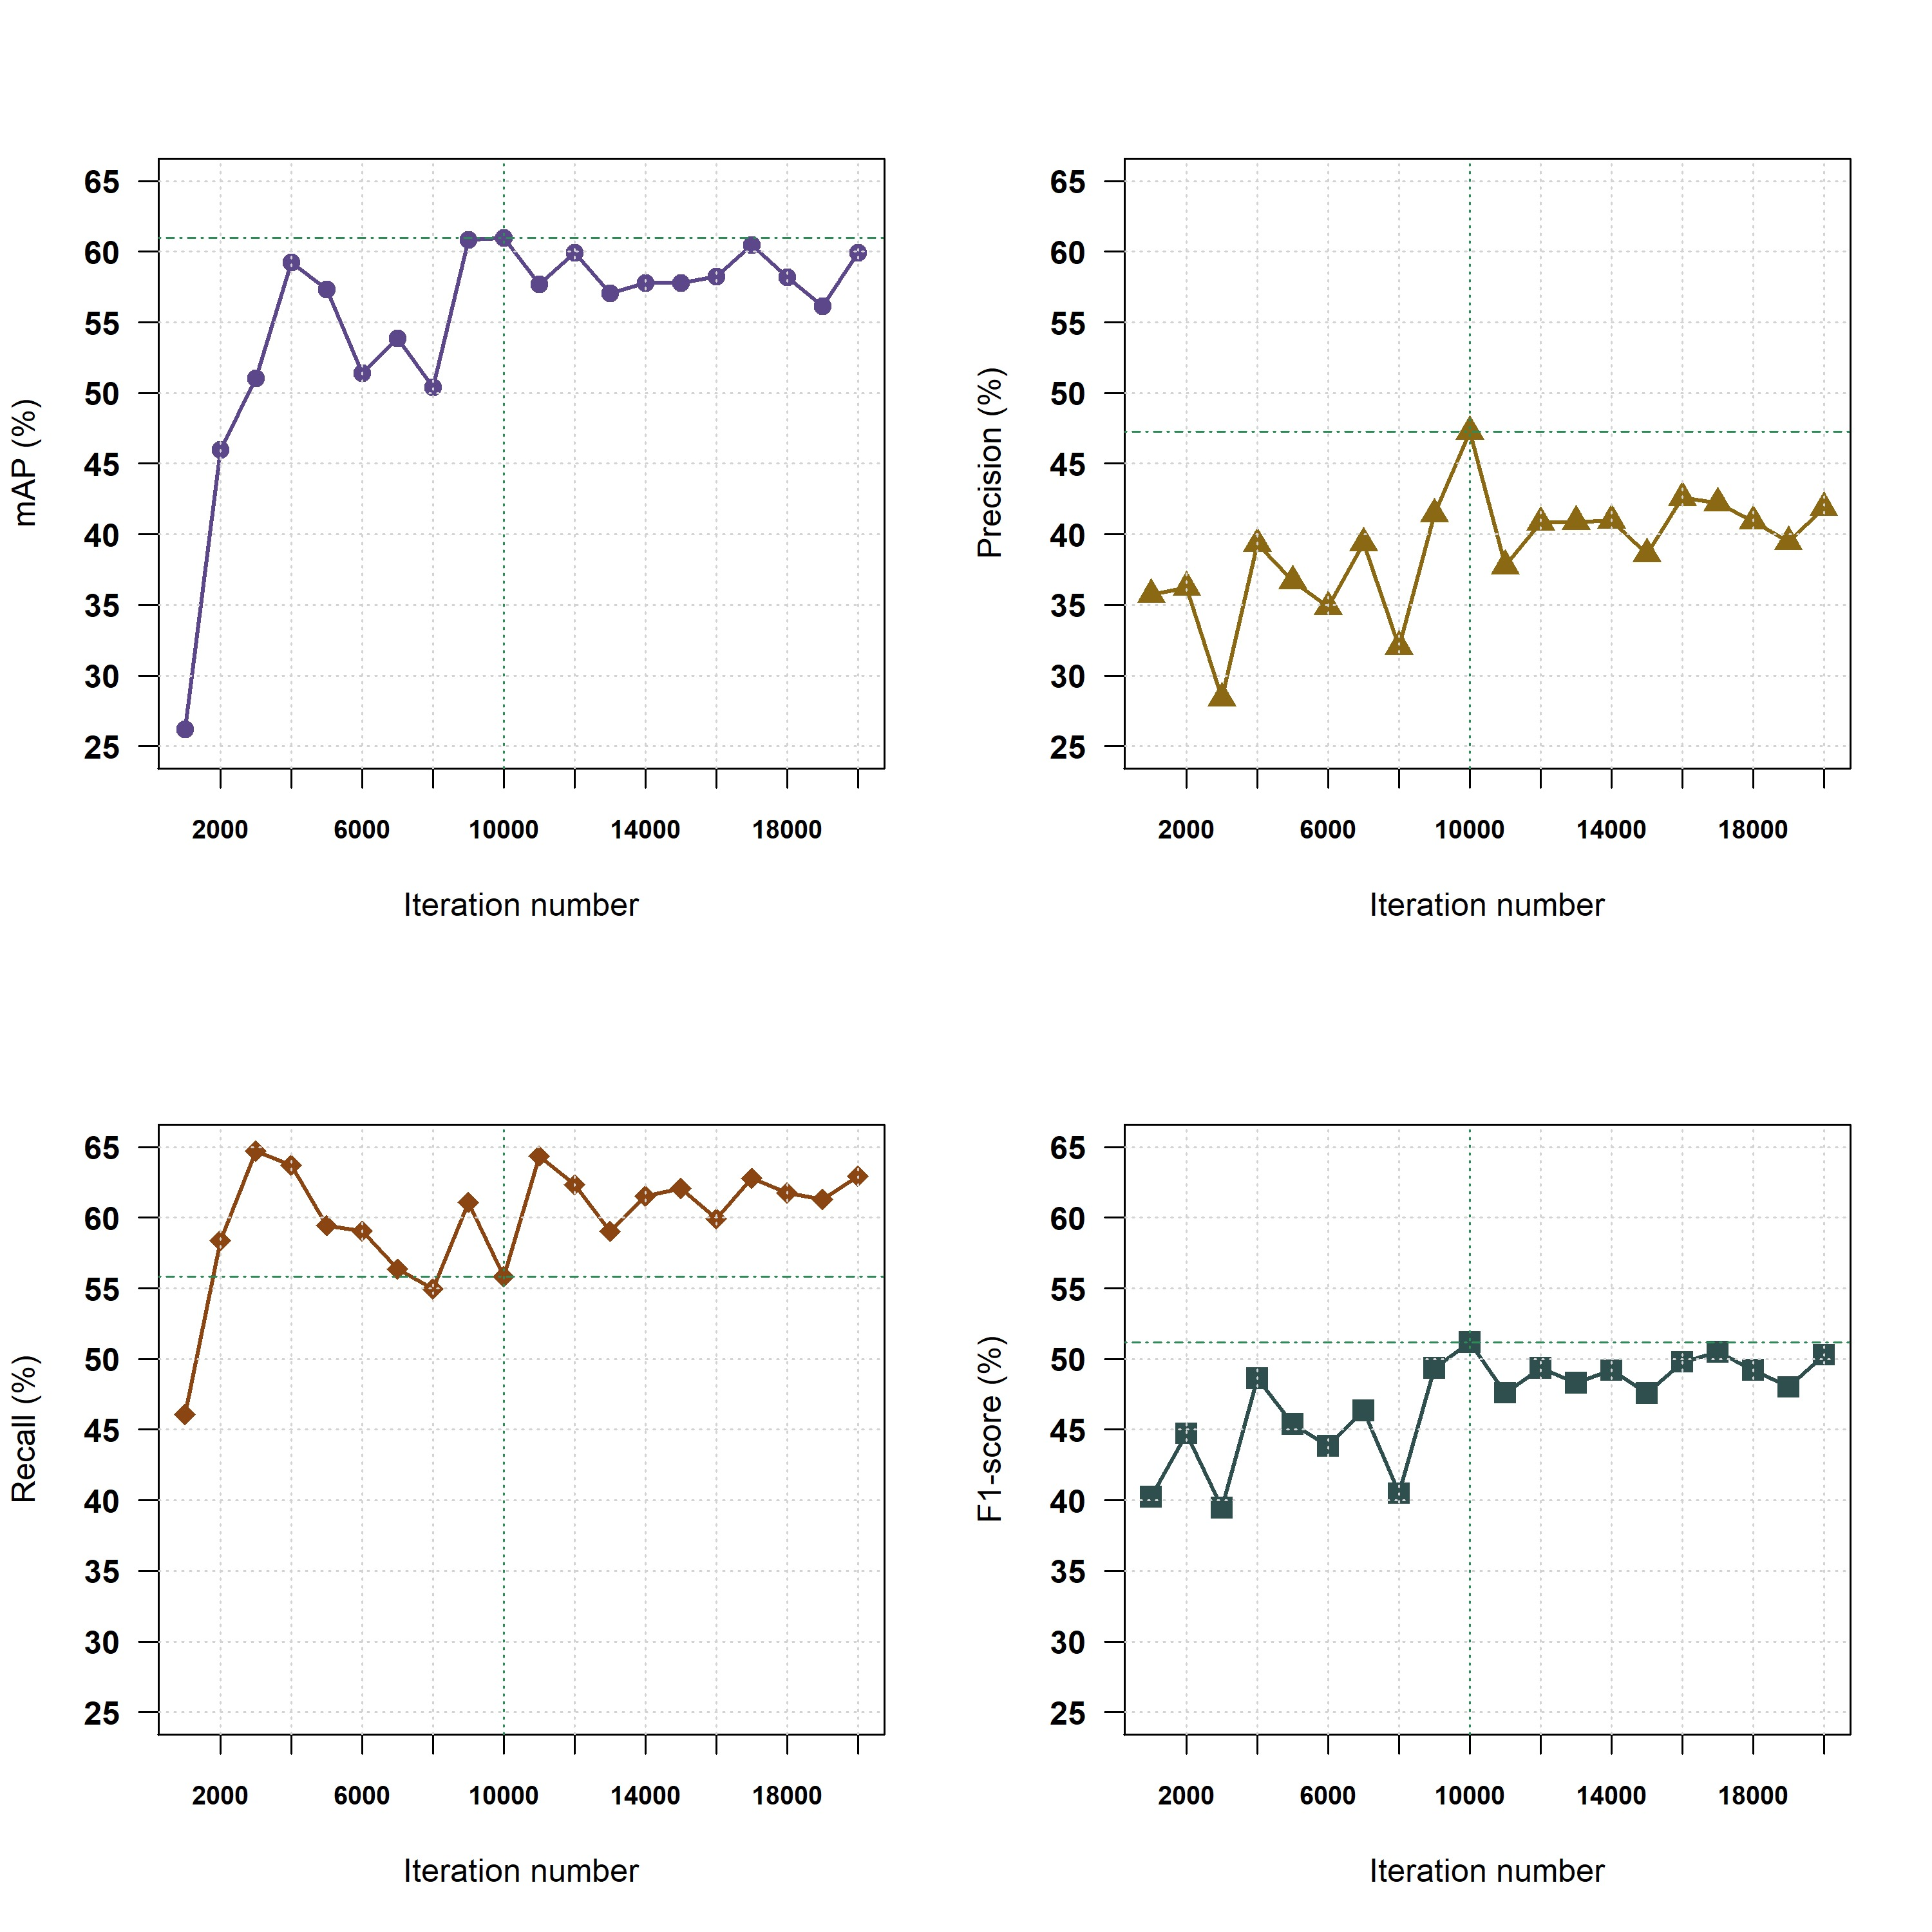
\includegraphics[width=0.67\textwidth]{img/chapters/resultados/metricas/metrics-train2.png}
\caption{\label{fig:metrics-train2}Resumen métricas segundo entrenamiento de la red neuronal con el dataset de OIDv4}
\end{figure}

Cabe detallar que, en los cálculos de las métricas de calidad de los dos entrenamientos que se han realizado se ha considerado un \textit{threshold} del \gls{iou} del 0,5. Evidentemente, al aumentar el \textit{threshold} a otros valores típicos como a 0,75 ó 0,95 disminuye drásticamente los valores del las métricas. Por norma general, cuando se ejecuta el detector de objetos de \gls{yolov4} el \textit{threshold} del \gls{iou} que viene definido por defecto es del 0,5. Es un valor suficientemente alto para considerar que la detección que se produce en cada fotograma de un vídeo es un \gls{tp}.

En vista a los resultados, no se han superado las métricas de calidad del dataset \gls{coco} sobre el que se entrenó \gls{yolov4}. Por tanto, se ha determinado continuar el proyecto con el modelo pre-entrenado de \gls{yolov4} con \gls{coco} como dataset de referencia.

\subsection{Métricas de calidad en MS COCO Dataset}
\label{subsec:metricas-calidad-coco}

En la siguiente tabla \ref{tab:metricas-clases-coco} se muestran los resultados obtenidos en la evaluación que se realizó en la sección \ref{sec:evaluate-cocodataset}. Las métricas más importantes sobre las clases de interés son las siguientes:

\begin{table}[ht]
\centering
\caption{Métricas de calidad de MS COCO en las clases de interés}
\label{tab:metricas-clases-coco}
\begin{tabular}{lccc}
\hline
\textbf{Class} & \textbf{AP(\%)} & \textbf{TP} & \textbf{FP} \\ \hline
Person         & 79,53           & 7.923       & 3.168       \\
Backpack       & 44,10           & 172         & 156         \\
Handbag        & 29,83           & 158         & 215         \\
Suitcase       & 71,08           & 205         & 102         \\ \hline
\end{tabular}
\end{table}

Como se contempla en la tabla \ref{tab:metricas-clases-coco}, excepto en la clase \texttt{Handbag}, se obtuvieron más \gls{tp} que \gls{fp} en las demás clases. El valor de \gls{ap} en la clase \texttt{Person} es muy superior al obtenido durante los entrenamientos en el dataset personalizado. Por el contrario, en las clases \texttt{Backpack, Handbag} y \texttt{Suitcase} se obtuvieron valores más bajos que en el primer entrenamiento con el dataset \gls{oidv4}.

En las tablas \ref{tab:comparativa-metricas1} y \ref{tab:comparativa-metricas2} se puede comparar de mejor forma las métricas más importantes obtenidas en los dos entrenamientos realizados sobre el dataset \gls{yolov4} respecto a las métricas obtenidas en la evaluación de \gls{yolov4} sobre \gls{coco}. Destaca la superioridad \gls{tp} sobre los \gls{fp} de \gls{coco}, en concreto más del doble. En los dos entrenamientos se obtuvieron valores muchos más \gls{fp} que \gls{tp} causados por el mal entrenamiento de la clase \texttt{Person}.

Llama la atención que se superó el valor de \gls{map} de \gls{coco} en el primer entrenamiento de \gls{oidv4}, a causa de los altos valores de \gls{ap} obtenidos en las clases de objetos que no eran personas. Sin embargo, en ninguno de los entrenamientos se igualó el valor del average \gls{iou} de \gls{coco}. Respecto a la precisión, Recall y F-score, si bien no se obtuvieron malos resultados en los dos últimos, no se superaron en ningún caso a los de \gls{coco}.

\begin{table}[ht]
\centering
\caption{Comparativa métricas de calidad entre los test en OIDv4 y MS COCO [1]}
\label{tab:comparativa-metricas1}
\begin{tabular}{lccc}
\hline
\textbf{Dataset}                   & \textbf{TP}          & \textbf{FP}          & \textbf{FN}          \\ \hline
\textbf{MS COCO}                   & \textbf{22.730}      & \textbf{10.889}      & \textbf{13.027}      \\
OIDv4 test 1                       & 430                  & 527                  & 273                  \\
OIDv4 test 2                       & 6.600                & 7.366                & 5.226                \\ \hline
\end{tabular}
\end{table}

\begin{table}[ht]
\centering
\caption{Comparativa métricas de calidad entre los dos test en OIDv4 y MS COCO [2]}
\label{tab:comparativa-metricas2}
\begin{tabular}{cccccc}
\hline
\textbf{Dataset}             & \textbf{\begin{tabular}[c]{@{}c@{}}Precision\\ (\%)\end{tabular}} & \textbf{\begin{tabular}[c]{@{}c@{}}Recall\\ (\%)\end{tabular}} & \textbf{\begin{tabular}[c]{@{}c@{}}F-score\\ (\%)\end{tabular}} & \textbf{\begin{tabular}[c]{@{}c@{}}average IoU\\ (\%)\end{tabular}} & \textbf{\begin{tabular}[c]{@{}c@{}}mAP @ 0.5\\ (\%)\end{tabular}} \\ \hline
\textbf{MS COCO}             & \textbf{67,61}                                                    & \textbf{63,57}                                                 & \textbf{65,53}                                                  & \textbf{56,04}                                                      & \textbf{64,16}                                                    \\
OIDv4 test 1                 & 44,93                                                             & 61,17                                                          & 51,81                                                           & 34,13                                                               & 66,25                                                             \\
OIDv4 test 2                 & 47,26                                                             & 55,81                                                          & 51,18                                                           & 37,83                                                               & 60,97                                                             \\ \hline
\end{tabular}
\end{table}

Los resultados en los entrenamientos no fueron satisfactorios y se ha continuado el proyecto con el modelo de \gls{yolov4} sobre el dataset \gls{coco}. Se ha llegado a la conclusión de que los datasets que han sido utilizados en los dos entrenamientos no contenían las imágenes idóneas para un correcta detección. Se ha observado que cuando las mochilas o bolsas de mano que se encontraban suspendidas en el suelo no se detectaban correctamente, dado que la mayoría de las imágenes de entrenamiento y validación son de mochilas que se encuentran perfectamente apoyadas en el suelo o las porta alguna persona. Por otro lado, las maletas de mano se han detectado correctamente ya que son equipajes típicamente rígidos que no muestran ninguna deformación, por lo que, aunque se encuentren en diferentes ángulos respecto a la visión de la cámara, las detecciones son eficientes.

Resultaría interesante evaluar las métricas en \gls{yolov4} sobre otros datasets que contengan un gran número de clases de los objetos de interés, o realizar un dataset con un conjunto de imágenes propias para esta aplicación, con el fin de determinar si se superan las métricas de \gls{coco}, teniendo en cuenta que el principal objetivo de este proyecto es la detección de objetos abandonados.

En el siguiente \href{https://drive.google.com/drive/folders/1ahdsjoDRICqDNB4dPGVYI6mVtYSDvvgu?usp=sharing}{link} se pueden acceder a los resultados obtenidos en la evaluación de las métricas de calidad tanto del dataset \gls{coco} como en la evaluación de los entrenamientos sobre el dataset \gls{oidv4}.

\subsection{Resultados en detección de objetos y personas con YOLOv4}
\label{subsec:resultados-yolov4-tf}

Antes de realizar pruebas y evaluar los resultados del algoritmo de detección de objetos abandonados con \gls{yolov4} y \gls{deepsort} se ha realizado en primera instancia una evaluación del algoritmo de detección de \gls{yolov4} con Tensorflow.

En la siguiente figura \ref{fig:gba-near-big3-detection-example} se muestran los resultados obtenidos en las detecciones sobre el dataset \gls{gba2018} \cite{gba-dataset}, donde se puede observar como la detección sobre las personas es muy buena, obteniéndose valores de \textit{confidence score} por encima del 90\%. Un problema muy común que ha ocurrido en la evaluación de todos los datasets con las clases \texttt{Handbag} y \texttt{Backpack} es que, como se puede observar en la primera imagen de la figura \ref{fig:gba-near-big3-detection-example}, en ocasiones el detector se confunde y realiza una doble detección con valores muy bajos de \textit{confidence score} sobre el objeto. Esto resulta un gran inconveniente a la hora de realizar la asociación persona-objeto en el algoritmo de detección de objetos abandonados, ya que en esas ocasiones se pierde con mucha facilidad la detección y en consecuencia hay muchos cambios de identidad. Otro problema, pero menos común, que se ha encontrado es cuando una mochila de dimensiones reducidas se encuentra apoyada en el suelo. Como se aprecia en la segunda imagen de la figura \ref{fig:gba-near-big3-detection-example}, el detector de objetos confunde la clase mochila con la clase perro. Típicamente las mochilas se detectan mejor cuando una persona la lleva encima.

\begin{figure}[ht]
\centering
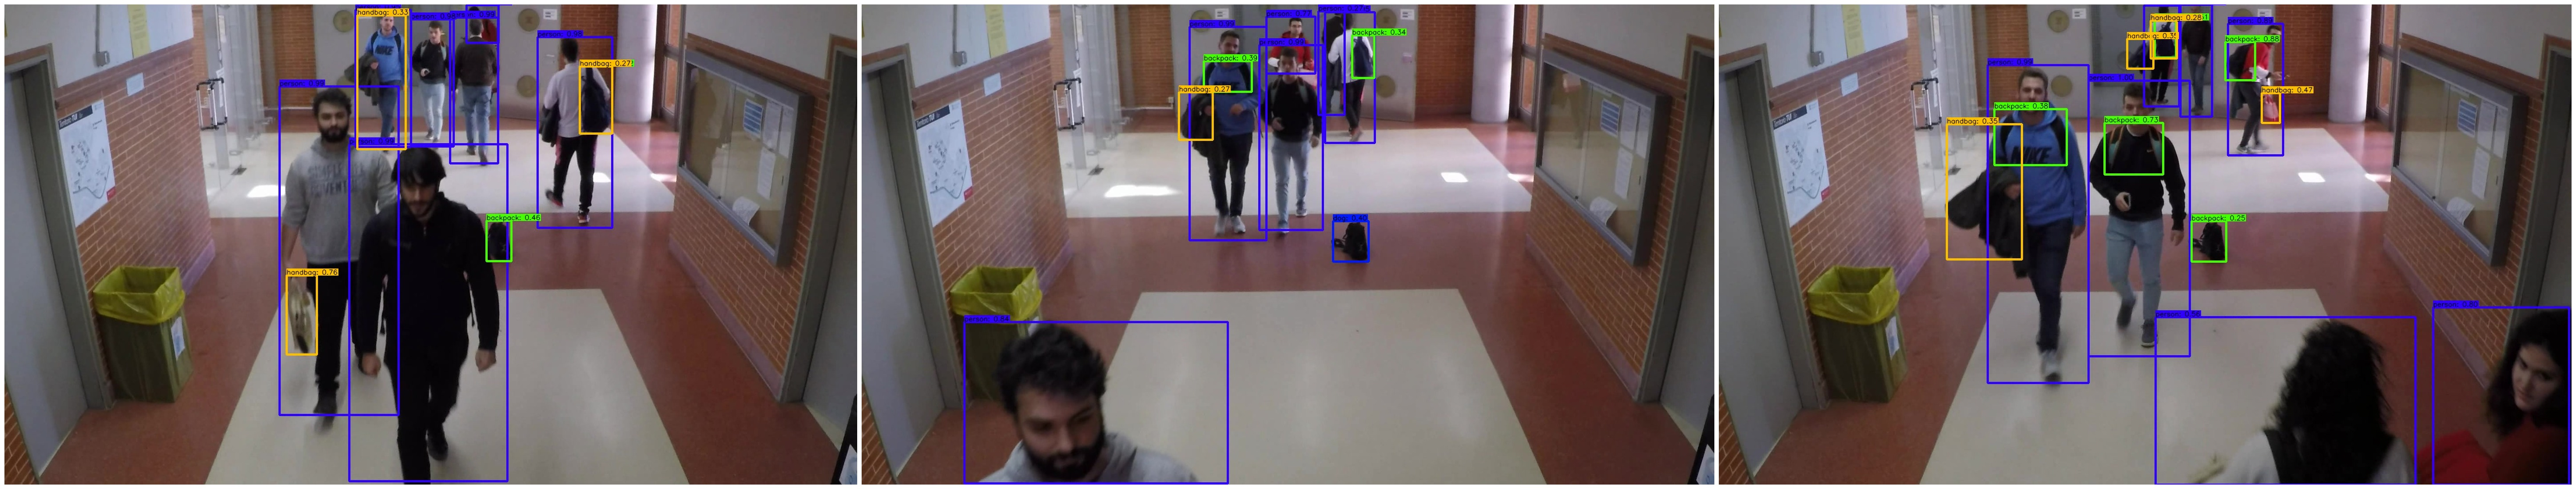
\includegraphics[width=0.85\textwidth]{img/chapters/resultados/deteccion/gba-near-big3-detection-example.jpg}
\caption{\label{fig:gba-near-big3-detection-example}Ejemplo 1 detección YOLOv4 Tensorflow \cite{gba-dataset}}
\end{figure}

En la siguiente figura \ref{fig:avss-easy-detection-example} se muestran los resultados obtenidos en las detecciones sobre el dataset \gls{avss} \cite{AVSSAB2007-dataset}, donde se puede observar como la detección en maletas son excelentes. En todas las evaluaciones que se han realizado del detector \gls{yolov4} sobre todos los datasets empleados se han obtenido elevados \textit{confidence score} para la clase \texttt{Suitcase}.

Se ha establecido un umbral de confianza mínima para todas las clases de $0,25$. Tal y como se puede ver en la última imagen de la figura \ref{fig:avss-easy-detection-example} no se estaba detectando la mochila porque no llegaba a ese umbral. No se ha disminuido el valor de este umbral de confianza dado que se obtenían muchos \gls{fp} sobre todas las clases.

\begin{figure}[ht]
\centering
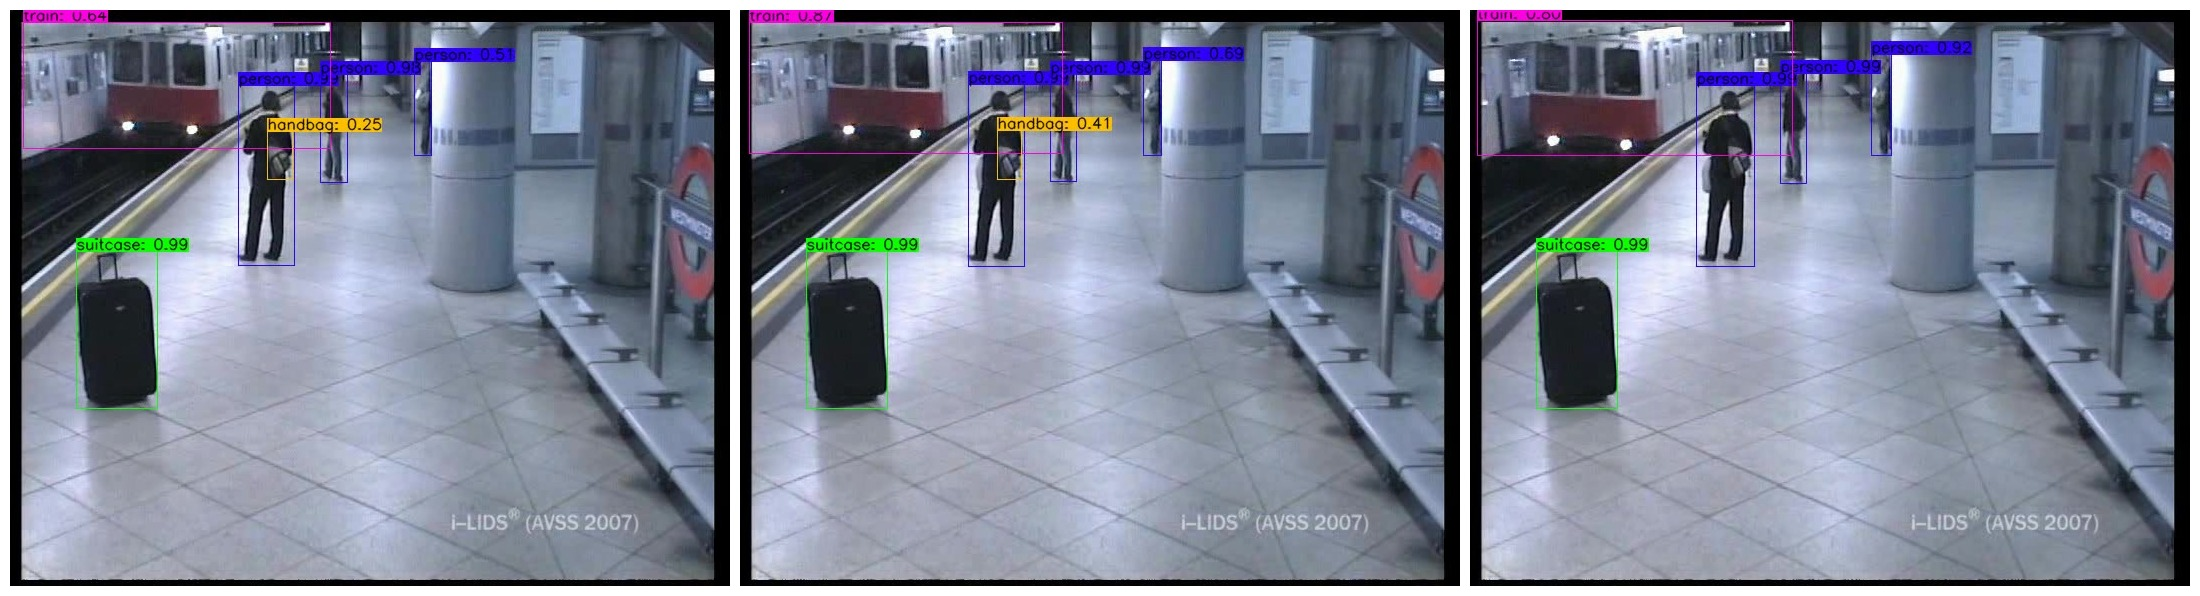
\includegraphics[width=0.85\textwidth]{img/chapters/resultados/deteccion/avss-easy-detection-example.jpg}
\caption{\label{fig:avss-easy-detection-example}Ejemplo 2 detección YOLOv4 Tensorflow \cite{AVSSAB2007-dataset}}
\end{figure}

En la siguiente figura \ref{fig:aboda-video5-detection-example} se ilustran los resultados obtenidos en las detecciones sobre el dataset \gls{aboda} \cite{aboda-dataset}. Como se observa en la primera imagen, una de las dos personas que se encuentra en la parte inferior no se detecta y la otra se detecta con el \textit{confidence score} más bajo establecido. Por otro lado, la otra persona que se encuentra en un ángulo más favorable se detecta con un 40\% de \textit{confidence score}, valores muy alejados de los que se obtienen sobre la clase \texttt{Person} en las evaluaciones de otros datasets.

Esta secuencia del dataset \gls{aboda} es un claro ejemplo de la gran influencia que tiene los cambios drásticos de iluminación, la distancia, el ángulo y la resolución de la cámara. En escenarios como el de esta secuencia se debe de entrenar una \gls{cnn} con un conjunto de imágenes específico, teniendo en cuenta la posición donde se encontrará la cámara, así como su resolución, y por supuesto las condiciones lumínicas del entorno.

\begin{figure}[ht]
\centering
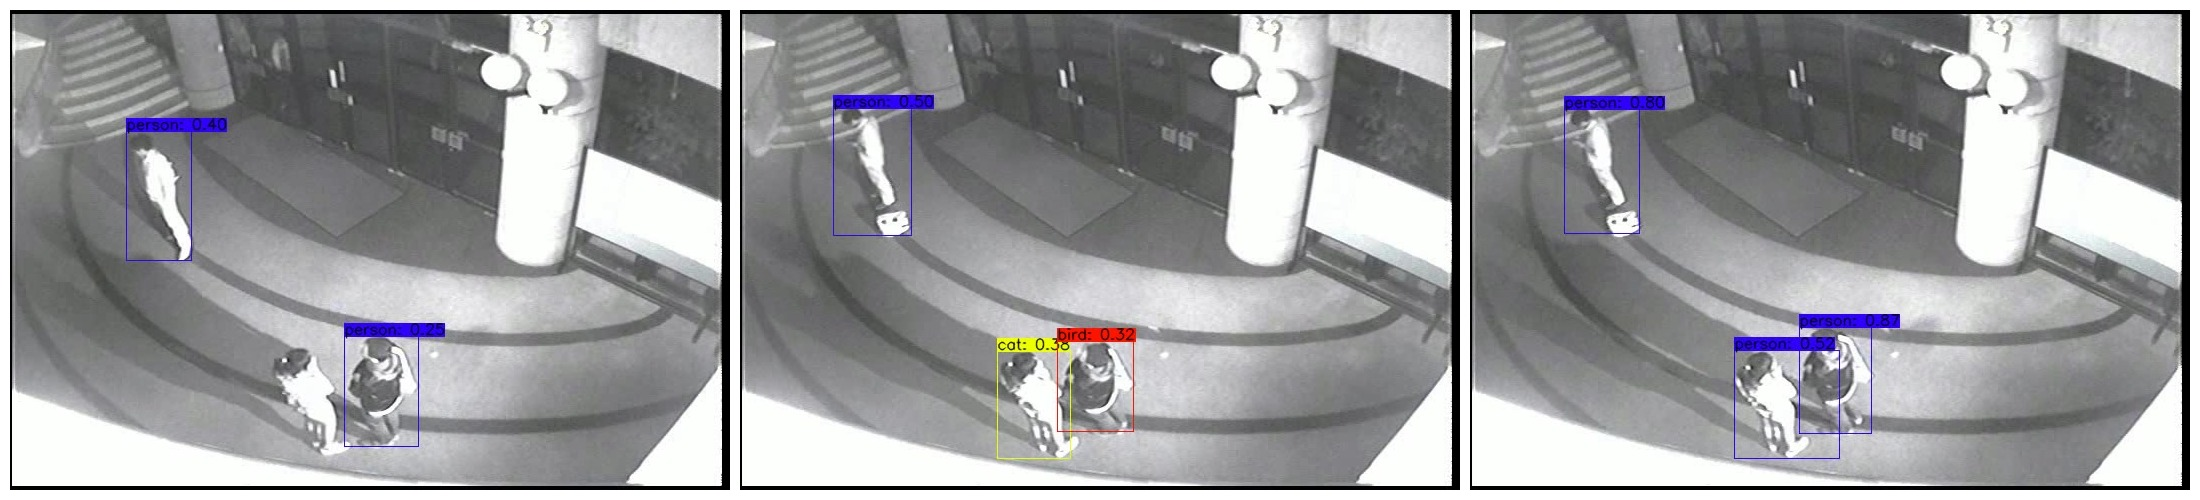
\includegraphics[width=0.85\textwidth]{img/chapters/resultados/deteccion/aboda-video5-detection-example.jpg}
\caption{\label{fig:aboda-video5-detection-example}Ejemplo 3 detección YOLOv4 Tensorflow \cite{aboda-dataset}}
\end{figure}

Todos los fotogramas han sido extraídos de las secuencias procesadas, las cuales se pueden acceder en el siguiente \href{https://drive.google.com/drive/folders/1hkUSC78H5moLyTqoNy0e0RhQTJSPt_um?usp=sharing}{link}.

\subsection{Resultados en seguimiento de objetos y personas con YOLOv4 y Deep SORT}
\label{subsec:resultados-yolov4+deepsort}

Las pruebas que se han realizado previas a la evaluación del algoritmo de detección de objetos abonados diseñado han sido el funcionamiento del algoritmo de seguimiento con \gls{deepsort} en los diferentes datasets. En la siguiente figura \ref{fig:avss-tracking-example} se aprecia como cada detección que ha realizado \gls{yolov4} se le ha asignado un número identificativo. Esto quiere decir que a cada elemento detectado, tanto personas como objetos de interés se le asigna una identidad única que va a servir para estudiar su posición a lo largo de los siguientes fotogramas. Los cuadros delimitadores verdes representan a las personas y los cuadros delimitadores de color azul representan los objetos de interés que se han filtrado en la etapa de detección.

En la figura se muestra un fragmento de una de las secuencias de vídeo del dataset \gls{avss} \cite{AVSSAB2007-dataset}. Siempre que no se producieran oclusiones prolongadas, el algoritmo trabajaba correctamente pudiendo rastrear objetos que en determinados momentos se salieran del plano. Como se puede observar en la primera imagen de la figura \ref{fig:avss-tracking-example}, la persona con número de identidad 93 pasa por detrás de la columna del andén, perdiéndose tanto la detección como el seguimiento. Sin embargo, fotogramas más tarde, cuando vuelve a aparecer al otro lado de la columna, se vuelve a detectar y se le asigna la identidad que tenía anteriormente. En las dos primeras imágenes de la figura se puede apreciar también la identidad que se le ha asignado a la bolsa de mano que aparece al final del andén, con el número identificativo 71.

En la última imagen de la figura se perciben cambios de identidad tanto de la persona que anteriormente tenía asignado como número de identidad el 93, así como la bolsa de mano que ha pasado de tener el número 71 al 88. Si nos fijamos bien en las dos últimas imágenes de la figura se puede observar que lo que se ha producido con la persona es un intercambio de identidad con la persona que se encuentra a la derecha de la columna en la segunda imagen. Suele ser un problema muy común en el rastreo de personas y objetos cuando se producen oclusiones o desaparición de la detección durante un tiempo determinado.

\begin{figure}[ht]
\centering
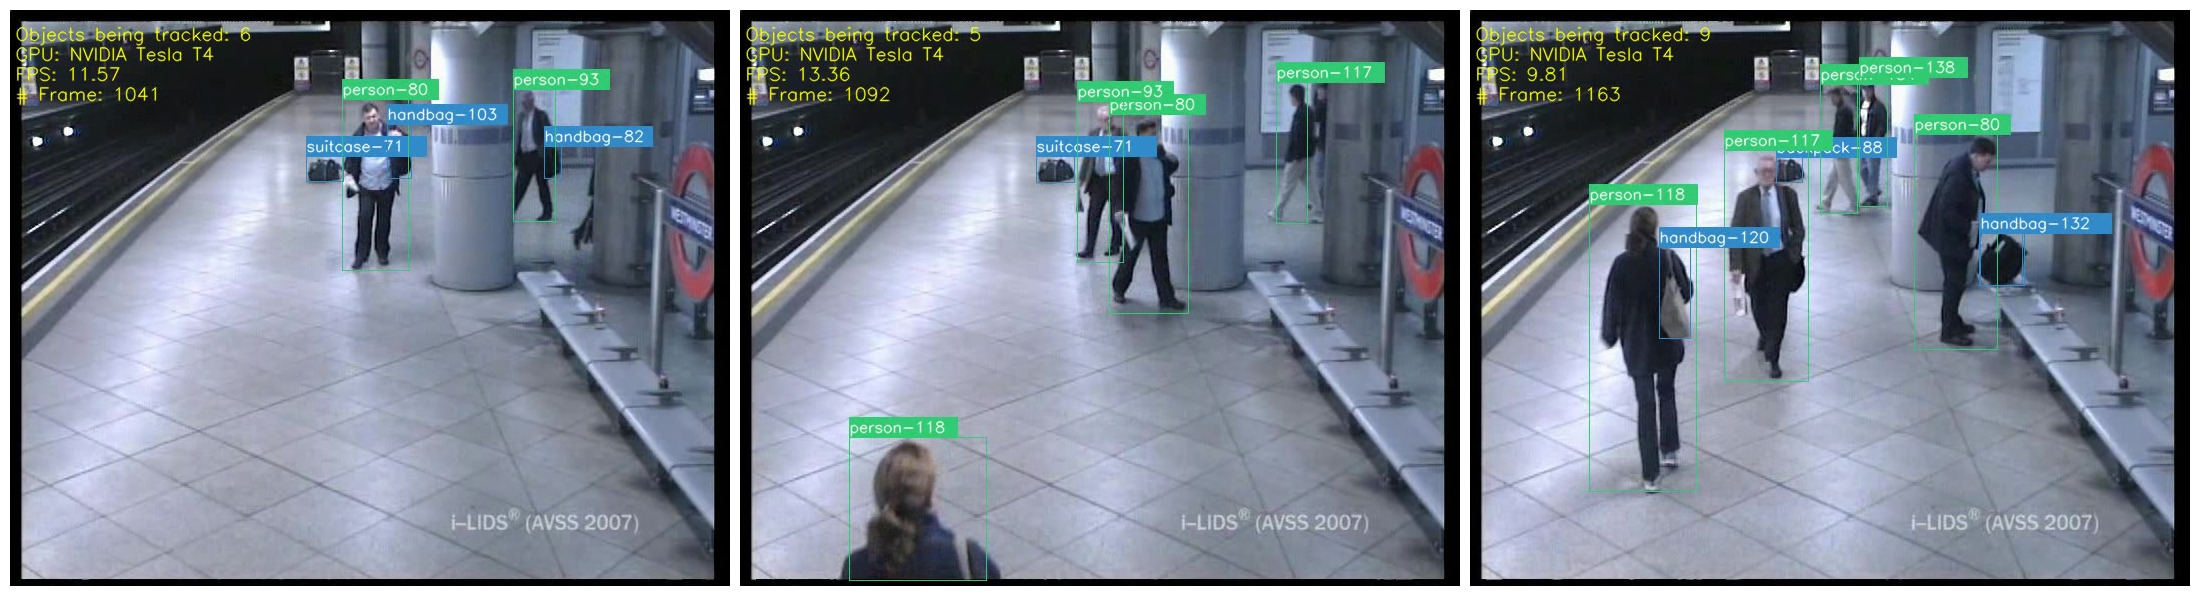
\includegraphics[width=0.85\textwidth]{img/chapters/resultados/tracking/avss-tracking-result-example.jpg}
\caption{\label{fig:avss-tracking-example}Ejemplo 1 seguimiento YOLOv4 y Deep Sort \cite{AVSSAB2007-dataset}}
\end{figure}

En la siguiente figura \ref{fig:gba-tracking-example} se observa claramente uno de los mayores problemas con los que nos hemos encontrado en el desarrollo del algoritmo de detección de objetos abandonados y es el cambio repentino de identidad al perderse la detección durante una corta duración de tiempo. En la primera imagen se puede observar a una persona con número de identidad 3 que ha dejado en el pasillo de la cafetería de la \gls{eps} una bolsa de mano con número de identidad 6. Pocos fotogramas después, cuando el individuo vuelve para recoger la bolsa de la cual es propietario, aparece con un nuevo número de identidad, ya que cuando se encontraba al fondo del pasillo se perdió la detección y se le asignó un nuevo número identificativo. Además, al recoger la bolsa del mano que se encontraba en el suelo, debido a los cambios de ángulos y deformaciones que se producen en la bolsa, se pierde la detección y tanto el algoritmo de detección como el algoritmo de rastreo determinan que esa bolsa de mano se trata de un nuevo objeto.

\begin{figure}[ht]
\centering
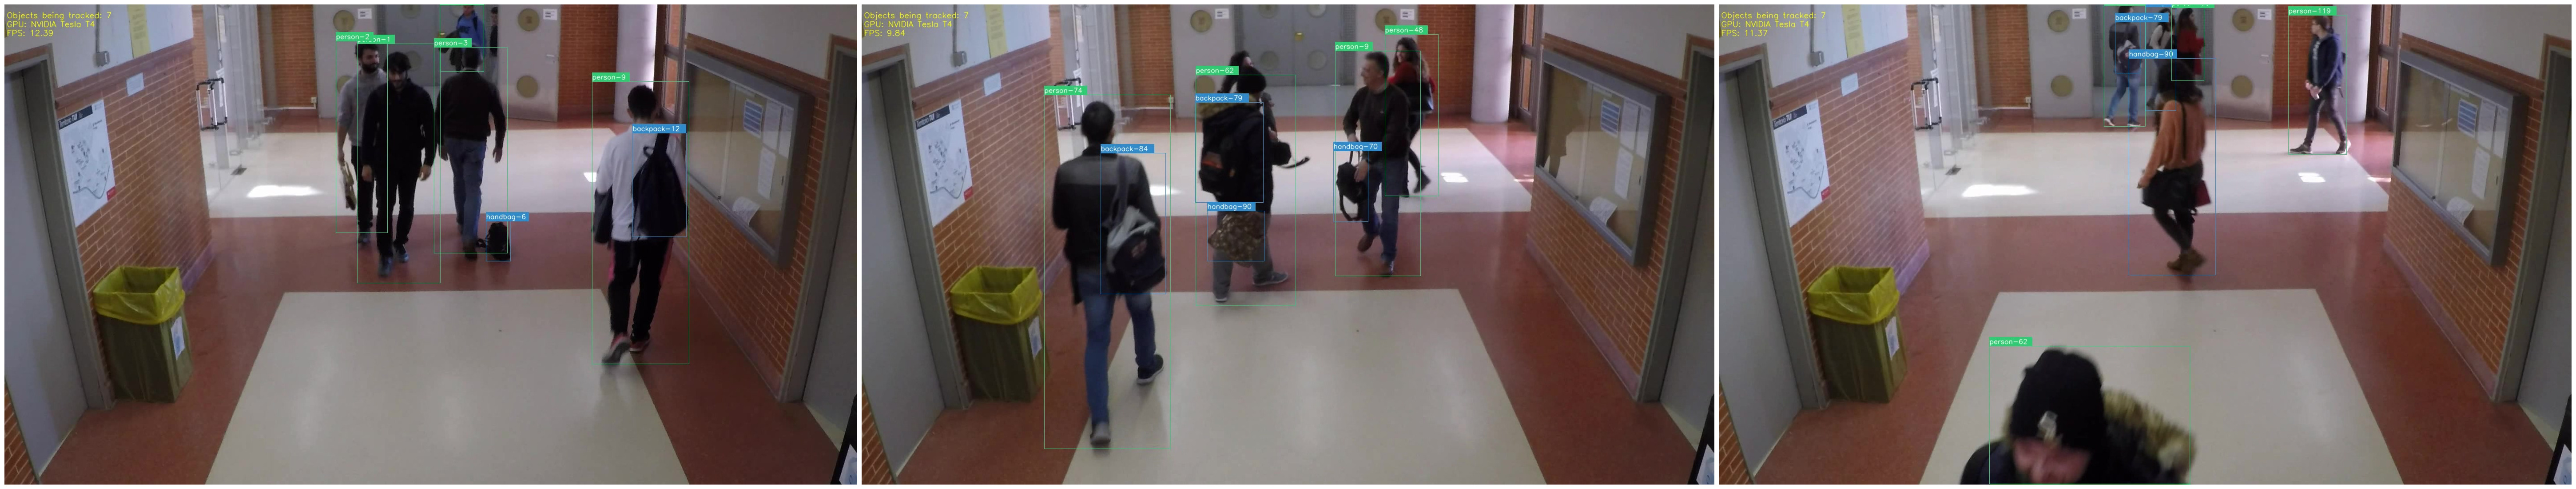
\includegraphics[width=0.85\textwidth]{img/chapters/resultados/tracking/gba-tracking-result-example.jpg}
\caption{\label{fig:gba-tracking-example}Ejemplo 2 seguimiento YOLOv4 y Deep Sort \cite{gba-dataset}}
\end{figure}

Con ello, se produce un cambio en el número identificativo del 6 al 70. Esto se trata de un grave problema a la hora de realizar la asociación persona-objeto en el algoritmo de detección de objetos abandonados. En muchos objetos, sobre todo en bolsas de mano, suelen tener asas y morfologías muy distintas al poder deformarlas al cogerlas o dejarlas en el suelo, que provocan que resulte muy difícil determinar que se sigue tratando del mismo objeto a lo largo de un número determinado de fotogramas. Este problema no aparece en maletas o equipajes de mano grandes y robustos, dado que no pierden su forma y resulta más fácil su identificación independientemente del ángulo en el que se encuentren.

Otro problema ajeno a la etapa de detección totalmente dependiente del algoritmo de seguimiento y que ocurre con relativa frecuencia en secuencias de vídeo de grandes aglomeraciones de personas y obstáculos que provocan la pérdida de las detecciones durante breves instantes de tiempo, es el cambio de identidad entre personas y objetos. En la última imagen de la figura \ref{fig:gba-tracking-example} se observa como la mujer que se encuentra en el centro del pasillo se le ha asignado el número identificativo 90, la identidad de la bolsa de mano que portaba una persona en la segunda imagen de la figura.

La siguiente figura corresponde al análisis del algoritmo de seguimiento sobre un fragmento de una de las secuencias de vídeo del dataset \gls{pets} \cite{pets2007-dataset}.

\begin{figure}[ht]
\centering
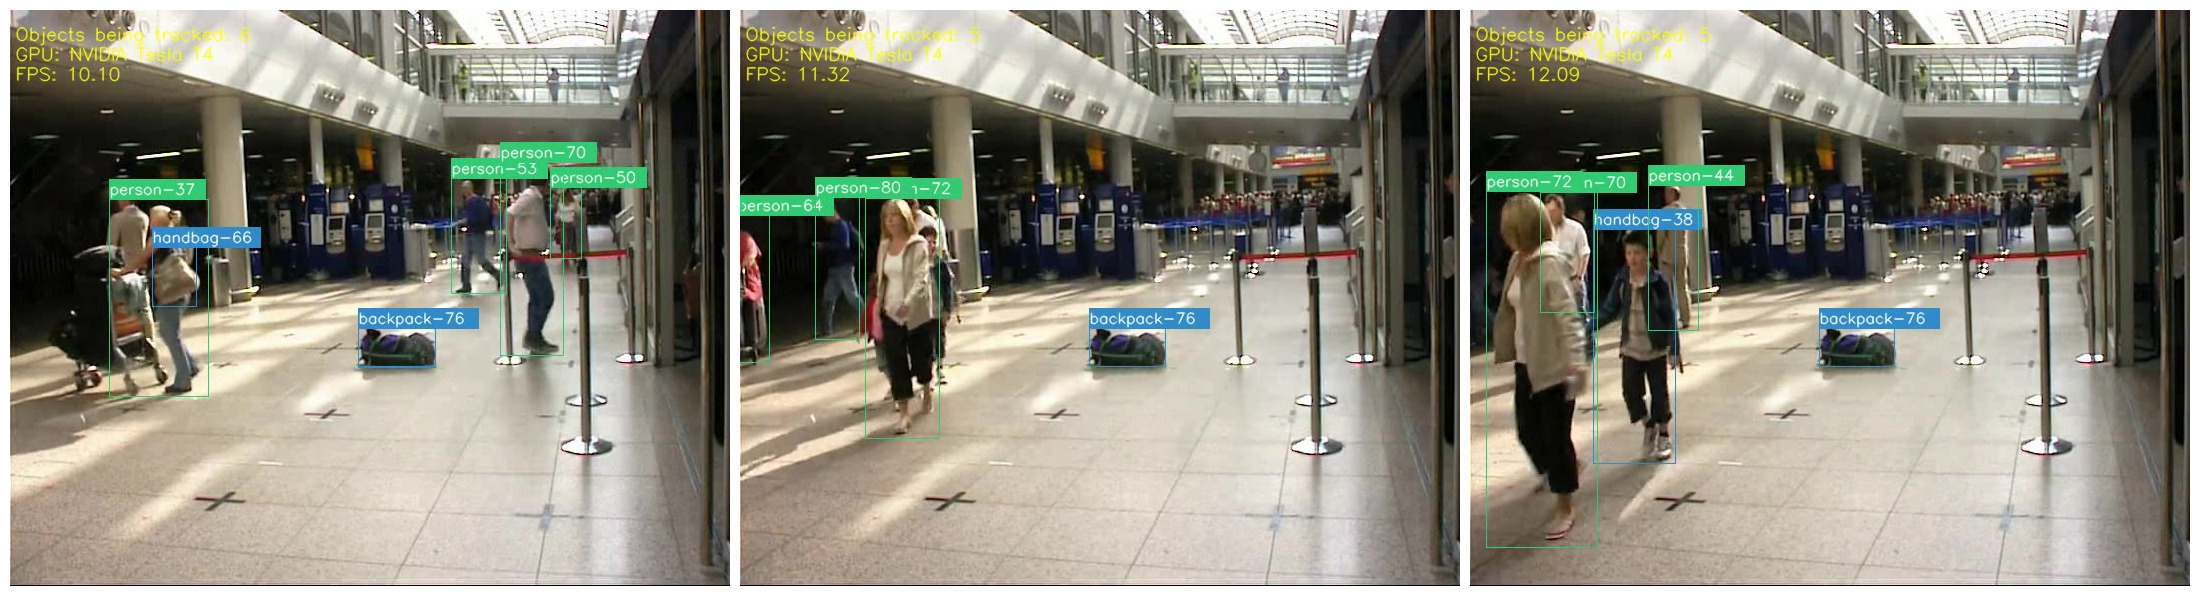
\includegraphics[width=0.85\textwidth]{img/chapters/resultados/tracking/pets-tracking-result-example.jpg}
\caption{\label{fig:pets2007-tracking-example}Ejemplo 3 seguimiento YOLOv4 y Deep Sort \cite{pets2007-dataset}}
\end{figure}

En esta figura \ref{fig:pets2007-tracking-example} se pueden observar nuevamente los dos grandes problemas que nos podemos encontrar en el seguimiento de objetos y personas, oclusiones o cambios de identidad y clases. En las dos primeras imágenes se pueden observar a dos mujeres con números de identidad 37 y 72 respectivamente, que se encuentran en un primer plano del área de detección de la cámara. Como se puede observar en ambas imágenes, estas dos personas están por delante de otras personas que se encuentran en planos posteriores, provocando oclusiones e impidiendo que se puedan detectar y rastrear. Por otro lado, se puede observar en la última imagen de la figura como, tras moverse la mujer que tenía como número identificativo el 72, aparece detectado y rastreado un niño al que se le está detectando como una bolsa de mano con número identificativo 38. Esto ha sucedido porque en fotogramas previos se detectó durante un instante de tiempo muy corto una bolsa de mano que se le asignó ese número de identidad y al desaparecer y aparecer el niño se le ha re-asignado esa identidad errónea.

Como se puede observar en todos los ejemplos descritos, a pesar de que \gls{deepsort} haya solucionado los graves problemas que tenía \gls{sort} en las oclusiones y en los cambios de identidad, este problema persiste en muchas ocasiones.

Todos los fotogramas han sido extraídos de las secuencias procesadas, las cuales se pueden acceder en el siguiente \href{https://drive.google.com/drive/folders/1MIfUcVmwIot6QgV0VRRu5PdFscV1Ma48?usp=sharing}{link}.

\subsection{Resultados en algoritmo de detección de objetos abandonados}
\label{subsec:resultados-abandon-algorithm}

Finalmente, tras comprobar el correcto funcionamiento de \gls{yolov4} como detector de objetos en el framework Tensorflow y evaluando su funcionamiento con el algoritmo de rastreo con \gls{deepsort}, se ha evaluado el desarrollo del algoritmo de detección de objetos abandonados en los distintos datasets descritos en la sección \ref{subsec:datasets-utilizados}.

En la siguiente figura \ref{fig:abandoned-avssab2007-example2} se aprecia un fragmento de una secuencia del dataset \gls{avss} \cite{AVSSAB2007-dataset}. En él se puede observar que tras los primeros segundos de vídeo se ha creado una asociación entre la persona con número de identidad 5 con la maleta que porta con número de identidad 2. Al fondo del andén se puede observar otra persona que se le ha asociado con número de identidad 3. Dado que la distancia respecto a la maleta con identidad 2 no es menor a 2 veces el ancho del cuadro delimitador de la persona, no se le ha asignado como propietario la maleta. No obstante, en el caso de que si que se cumpliera la distancia mínima a la que se le pudiera asignar la maleta, cobra mayor peso la mínima distancia que se encuentra respecto a una persona, que en este caso, como ya se ha comentado, es la persona con número de identidad 5.

En los siguientes fotogramas de la figura \ref{fig:abandoned-avssab2007-example2} se puede observar como la persona se está alejando de la maleta. En la segunda imagen de la segunda fila se puede observar que la persona se encuentra a una distancia 3 veces mayor a la distancia que se estableció como distancia de asociamiento, con lo cual, la maleta se encuentra en zona de alarma y se indica mediante cuadros delimitadores tanto en la persona como en la maleta, que ésta se encuentra en riesgo de ser abandonada.

En la segunda imagen de la tercera fila ya se puede ver que la persona ha sobrepasado la zona delimitada como zona de alarma, y ahora se encuentra a una distancia 5 veces mayor a la distancia de asociamiento. En este caso se ha establecido que es una distancia considerablemente grande para determinar que el objeto ha sido abandonado. En el caso de que no se hubiera llegado a esa distancia de abandono, pero la persona hubiera desaparecido del plano de la cámara, se habría determinado de igual manera que la maleta ha sido abandonada, es decir, en el momento en el que se pierda la asociación porque la identidad de la persona ya no es rastreada, se entiende que la persona ya no se encuentra en escena y ha quedado abandonado el objeto del cual es propietario.

\begin{figure}[ht]
\centering
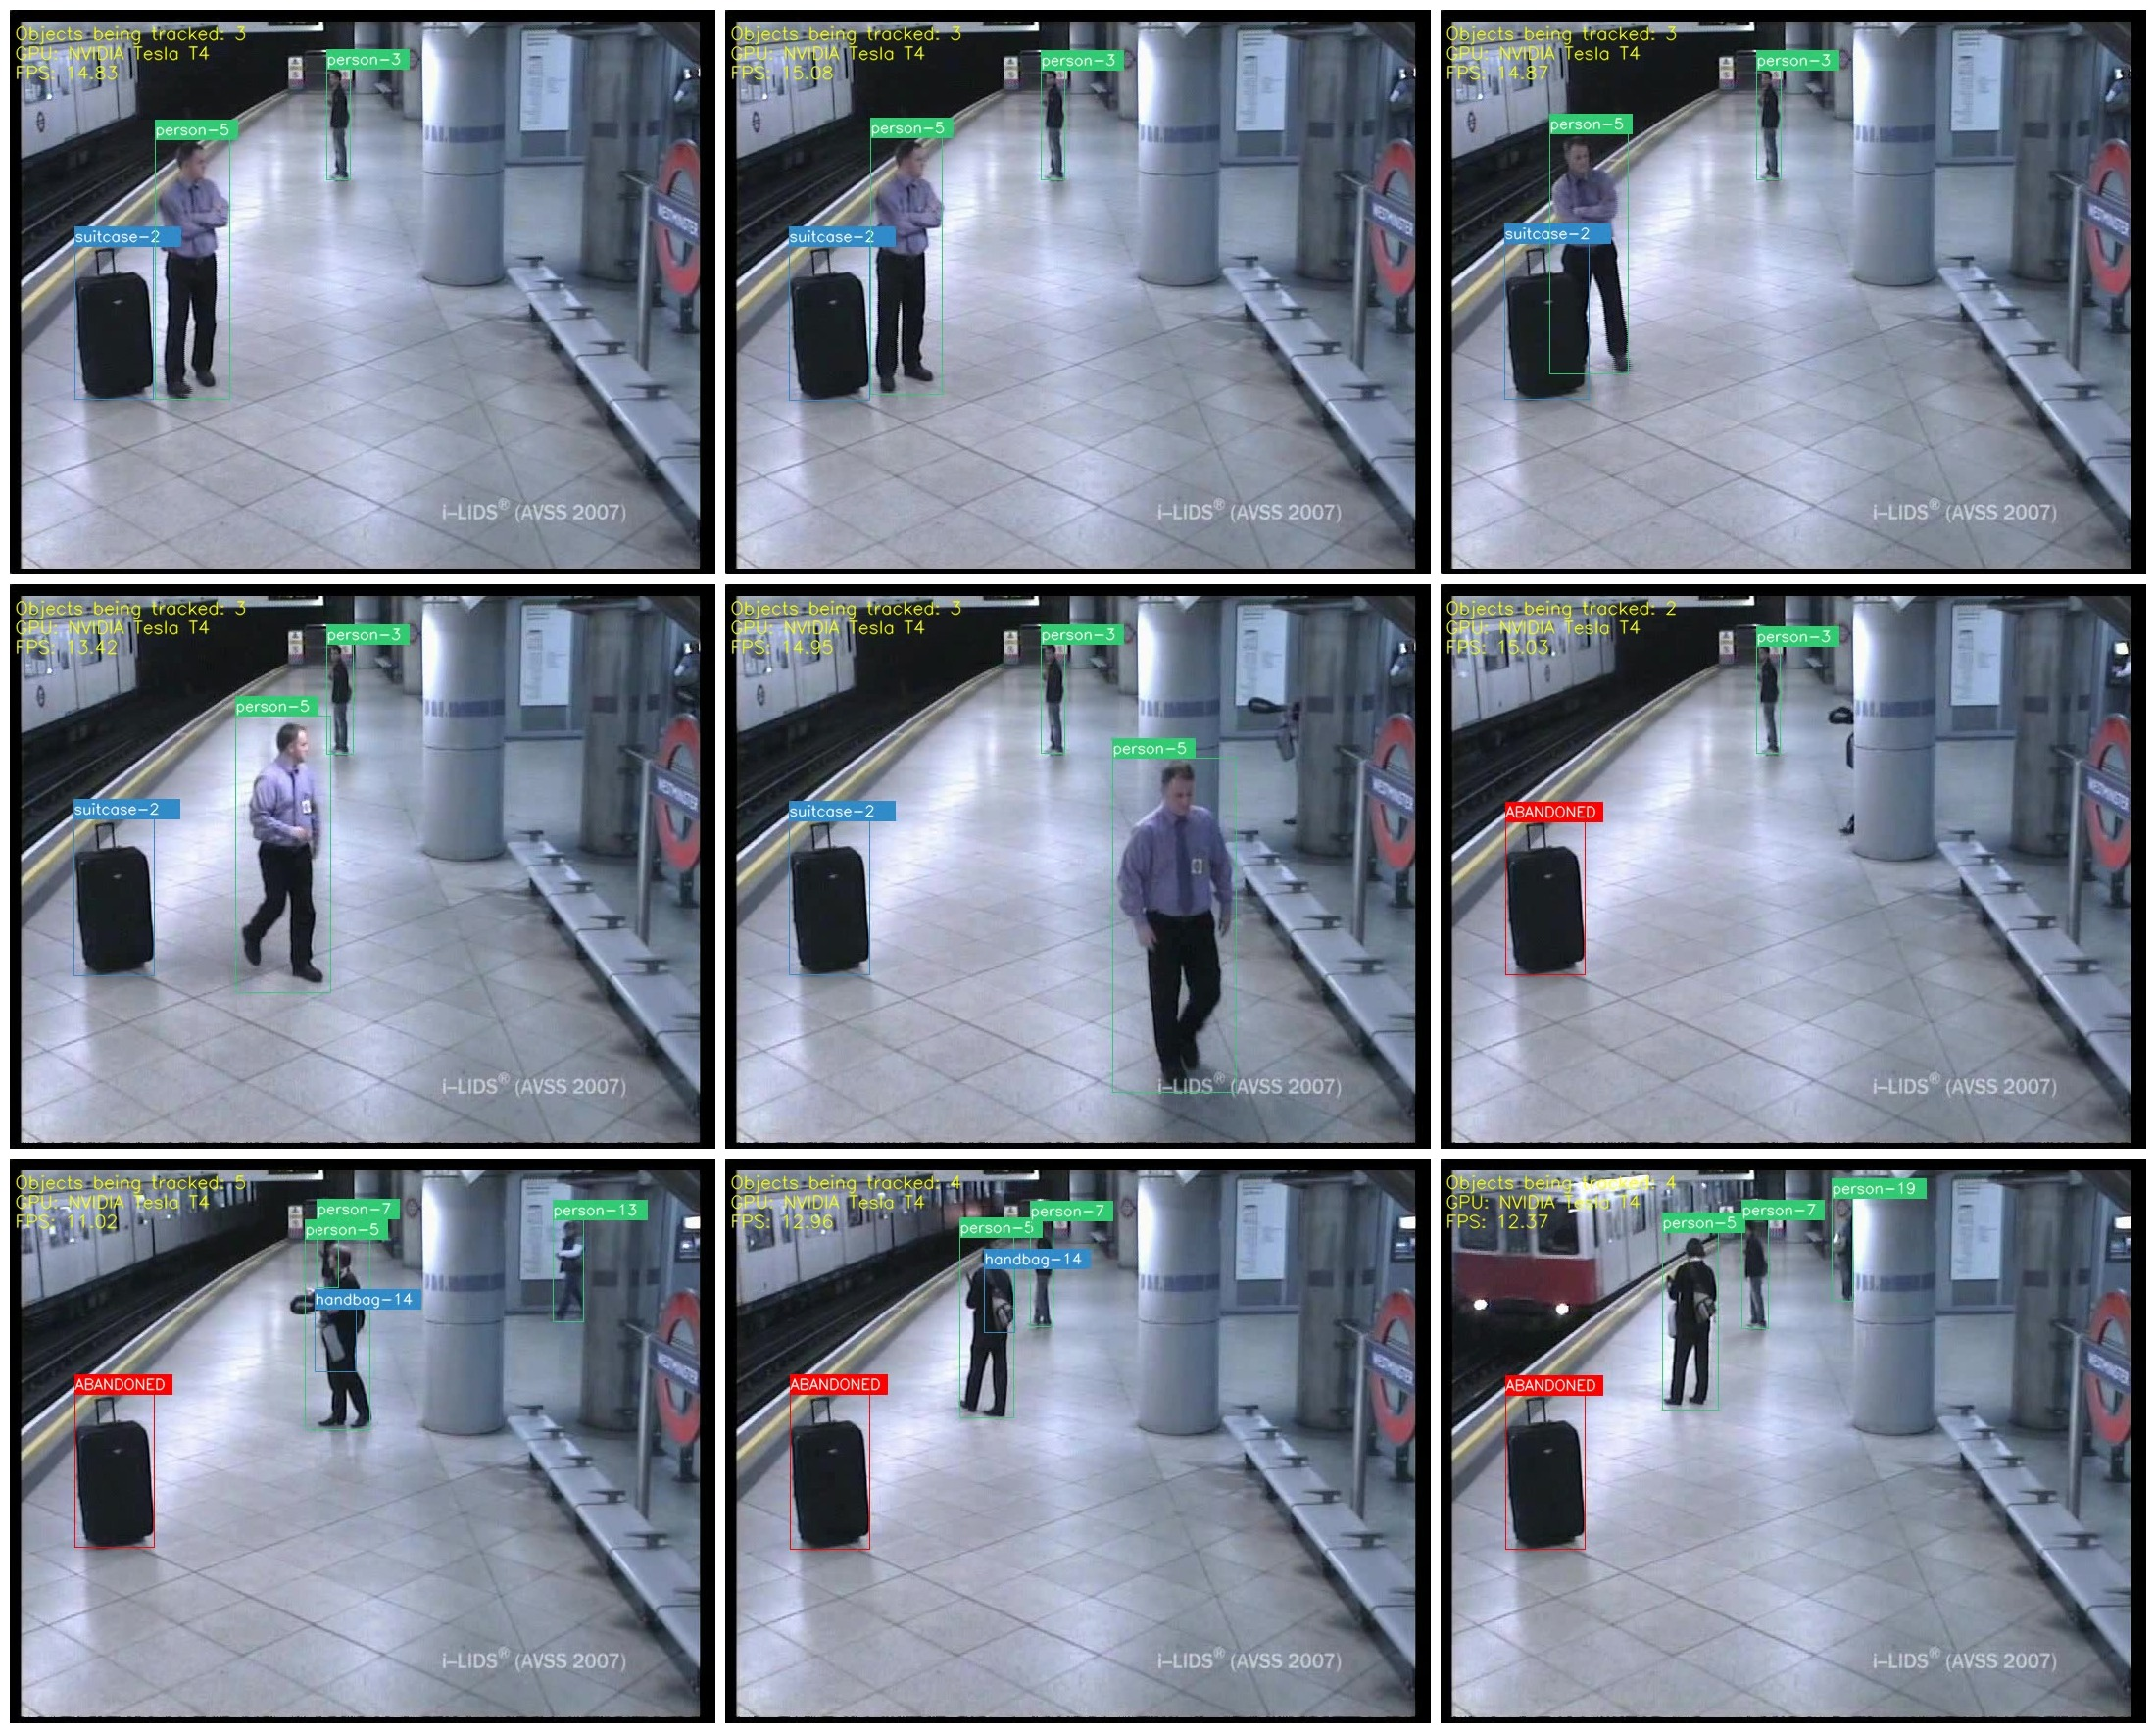
\includegraphics[width=0.85\textwidth]{img/chapters/resultados/abandono/abandoned-avssab2007-example2.png}
\caption{\label{fig:abandoned-avssab2007-example2}Individuo abandona su maleta en el la zona cercana del andén \cite{AVSSAB2007-dataset}}
\end{figure}

En la siguiente figura \ref{fig:abandoned-aboda-example1} se ilustra otro ejemplo similar al anterior. En este caso, se ha evaluado el algoritmo sobre la primera secuencia de vídeo del dataset \gls{aboda} \cite{aboda-dataset}.

\begin{figure}[ht]
\centering
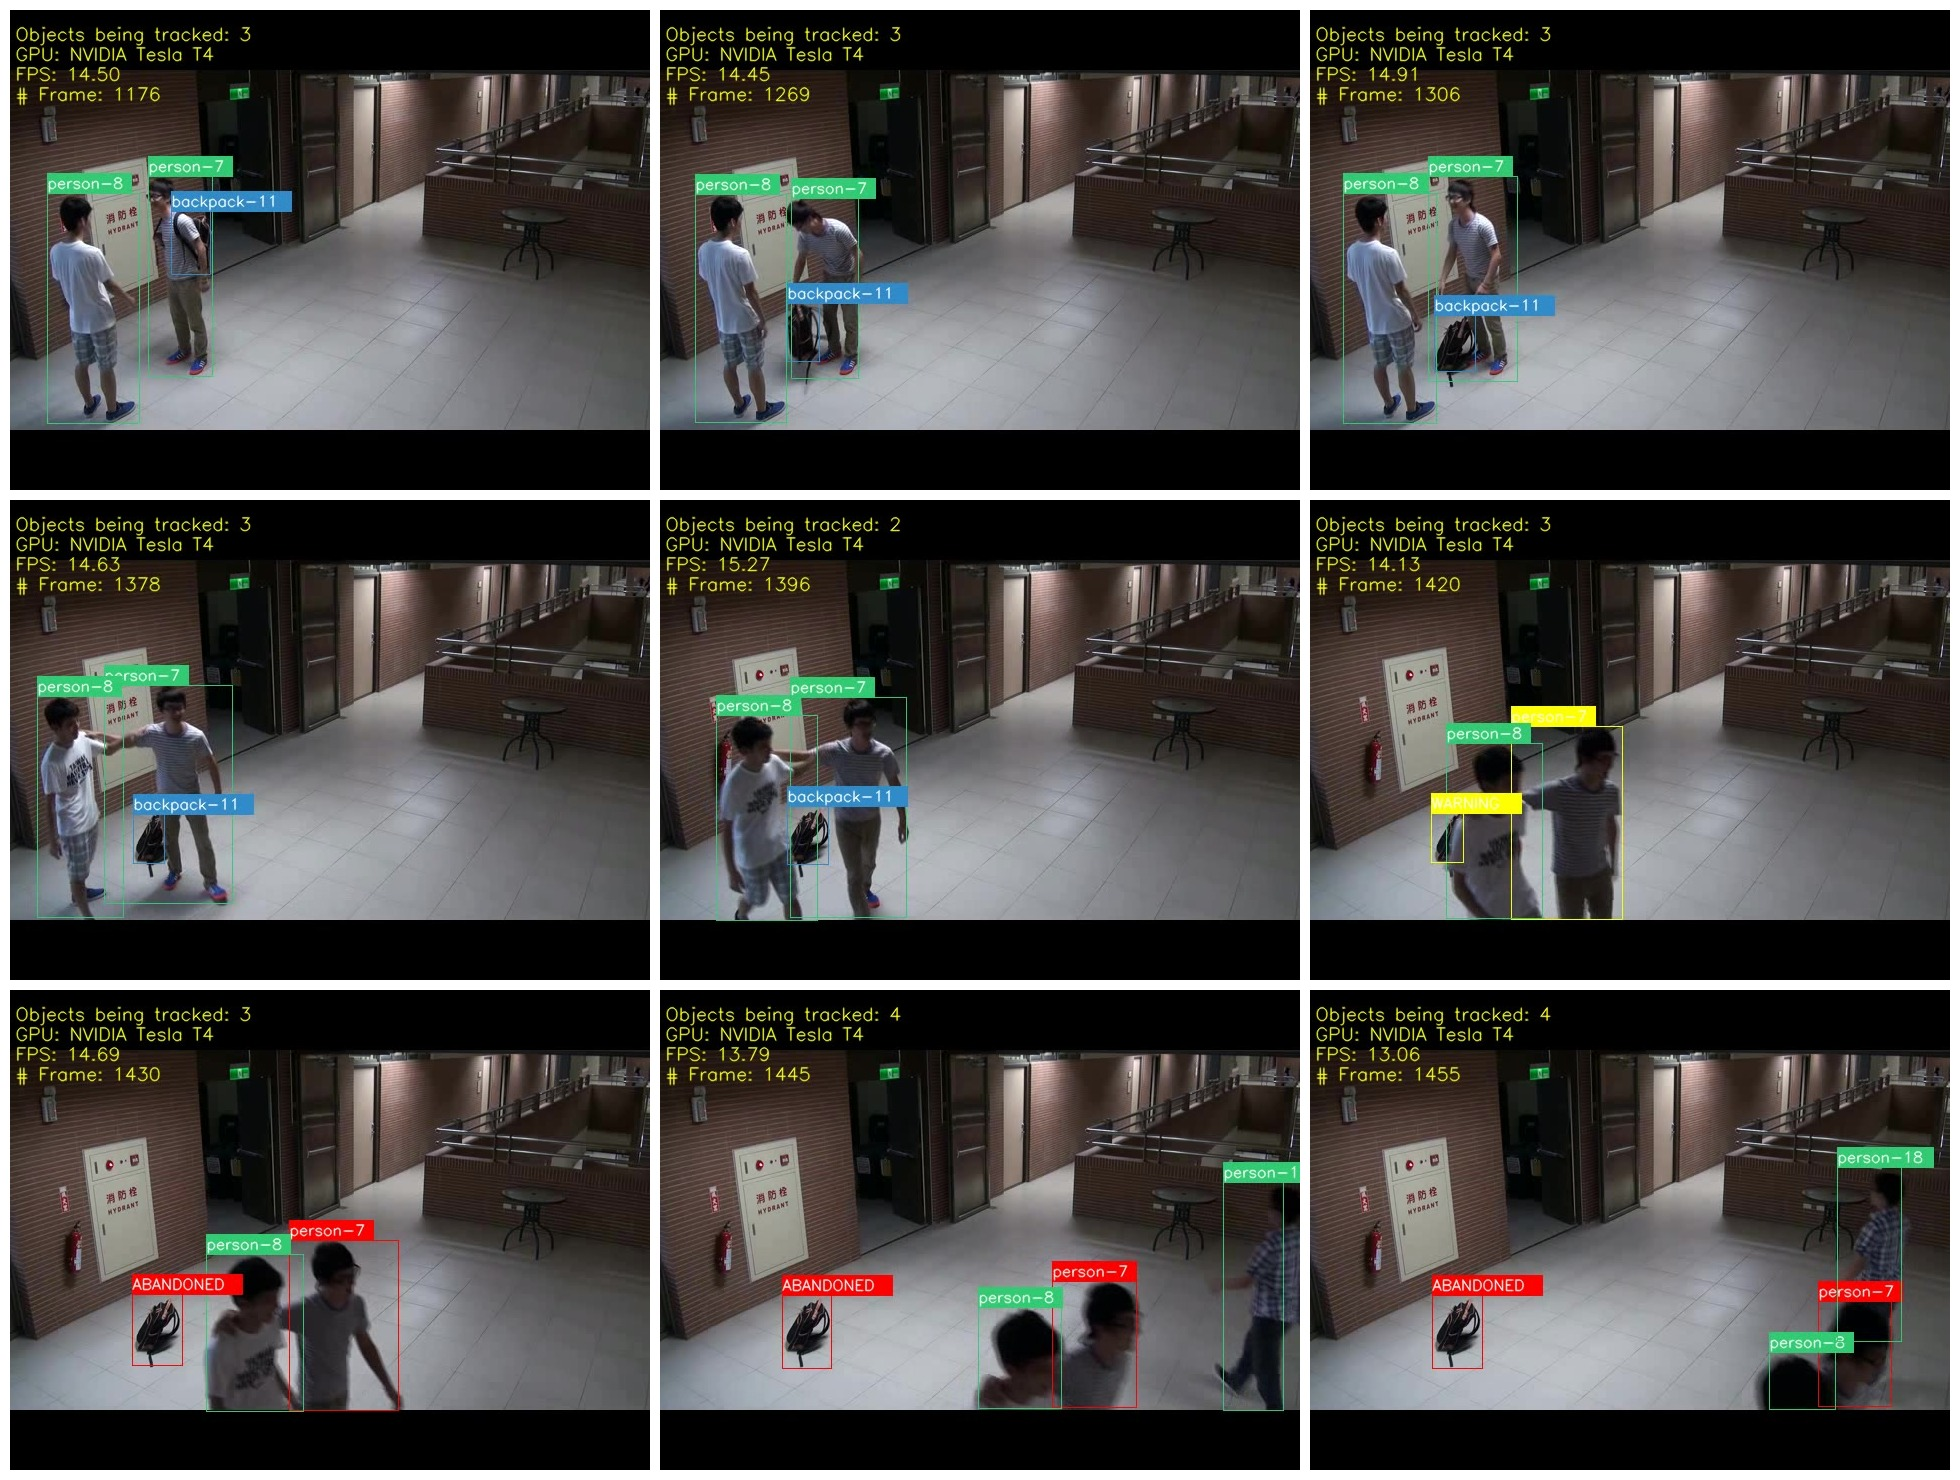
\includegraphics[width=0.85\textwidth]{img/chapters/resultados/abandono/abandoned-aboda-example1.png}
\caption{\label{fig:abandoned-aboda-example1}Individuo abandona su mochila en el hall de un edificio \cite{aboda-dataset}}
\end{figure}

En la escena se observan dos chicos jóvenes que se encuentran en el hall de un edificio y uno de ellos con número de identidad 7 porta una mochila con número de identidad 11. A pesar de que en el plano de visión también se encuentre otra persona, prima la mínima distancia entre mochila y persona, que en este caso es con la persona con identidad 7. Una vez creada la asociación se puede presenciar en los fotogramas siguientes como las dos personas abandonan el lugar dejando la mochila desatendida.

\begin{figure}[ht!]
\centering
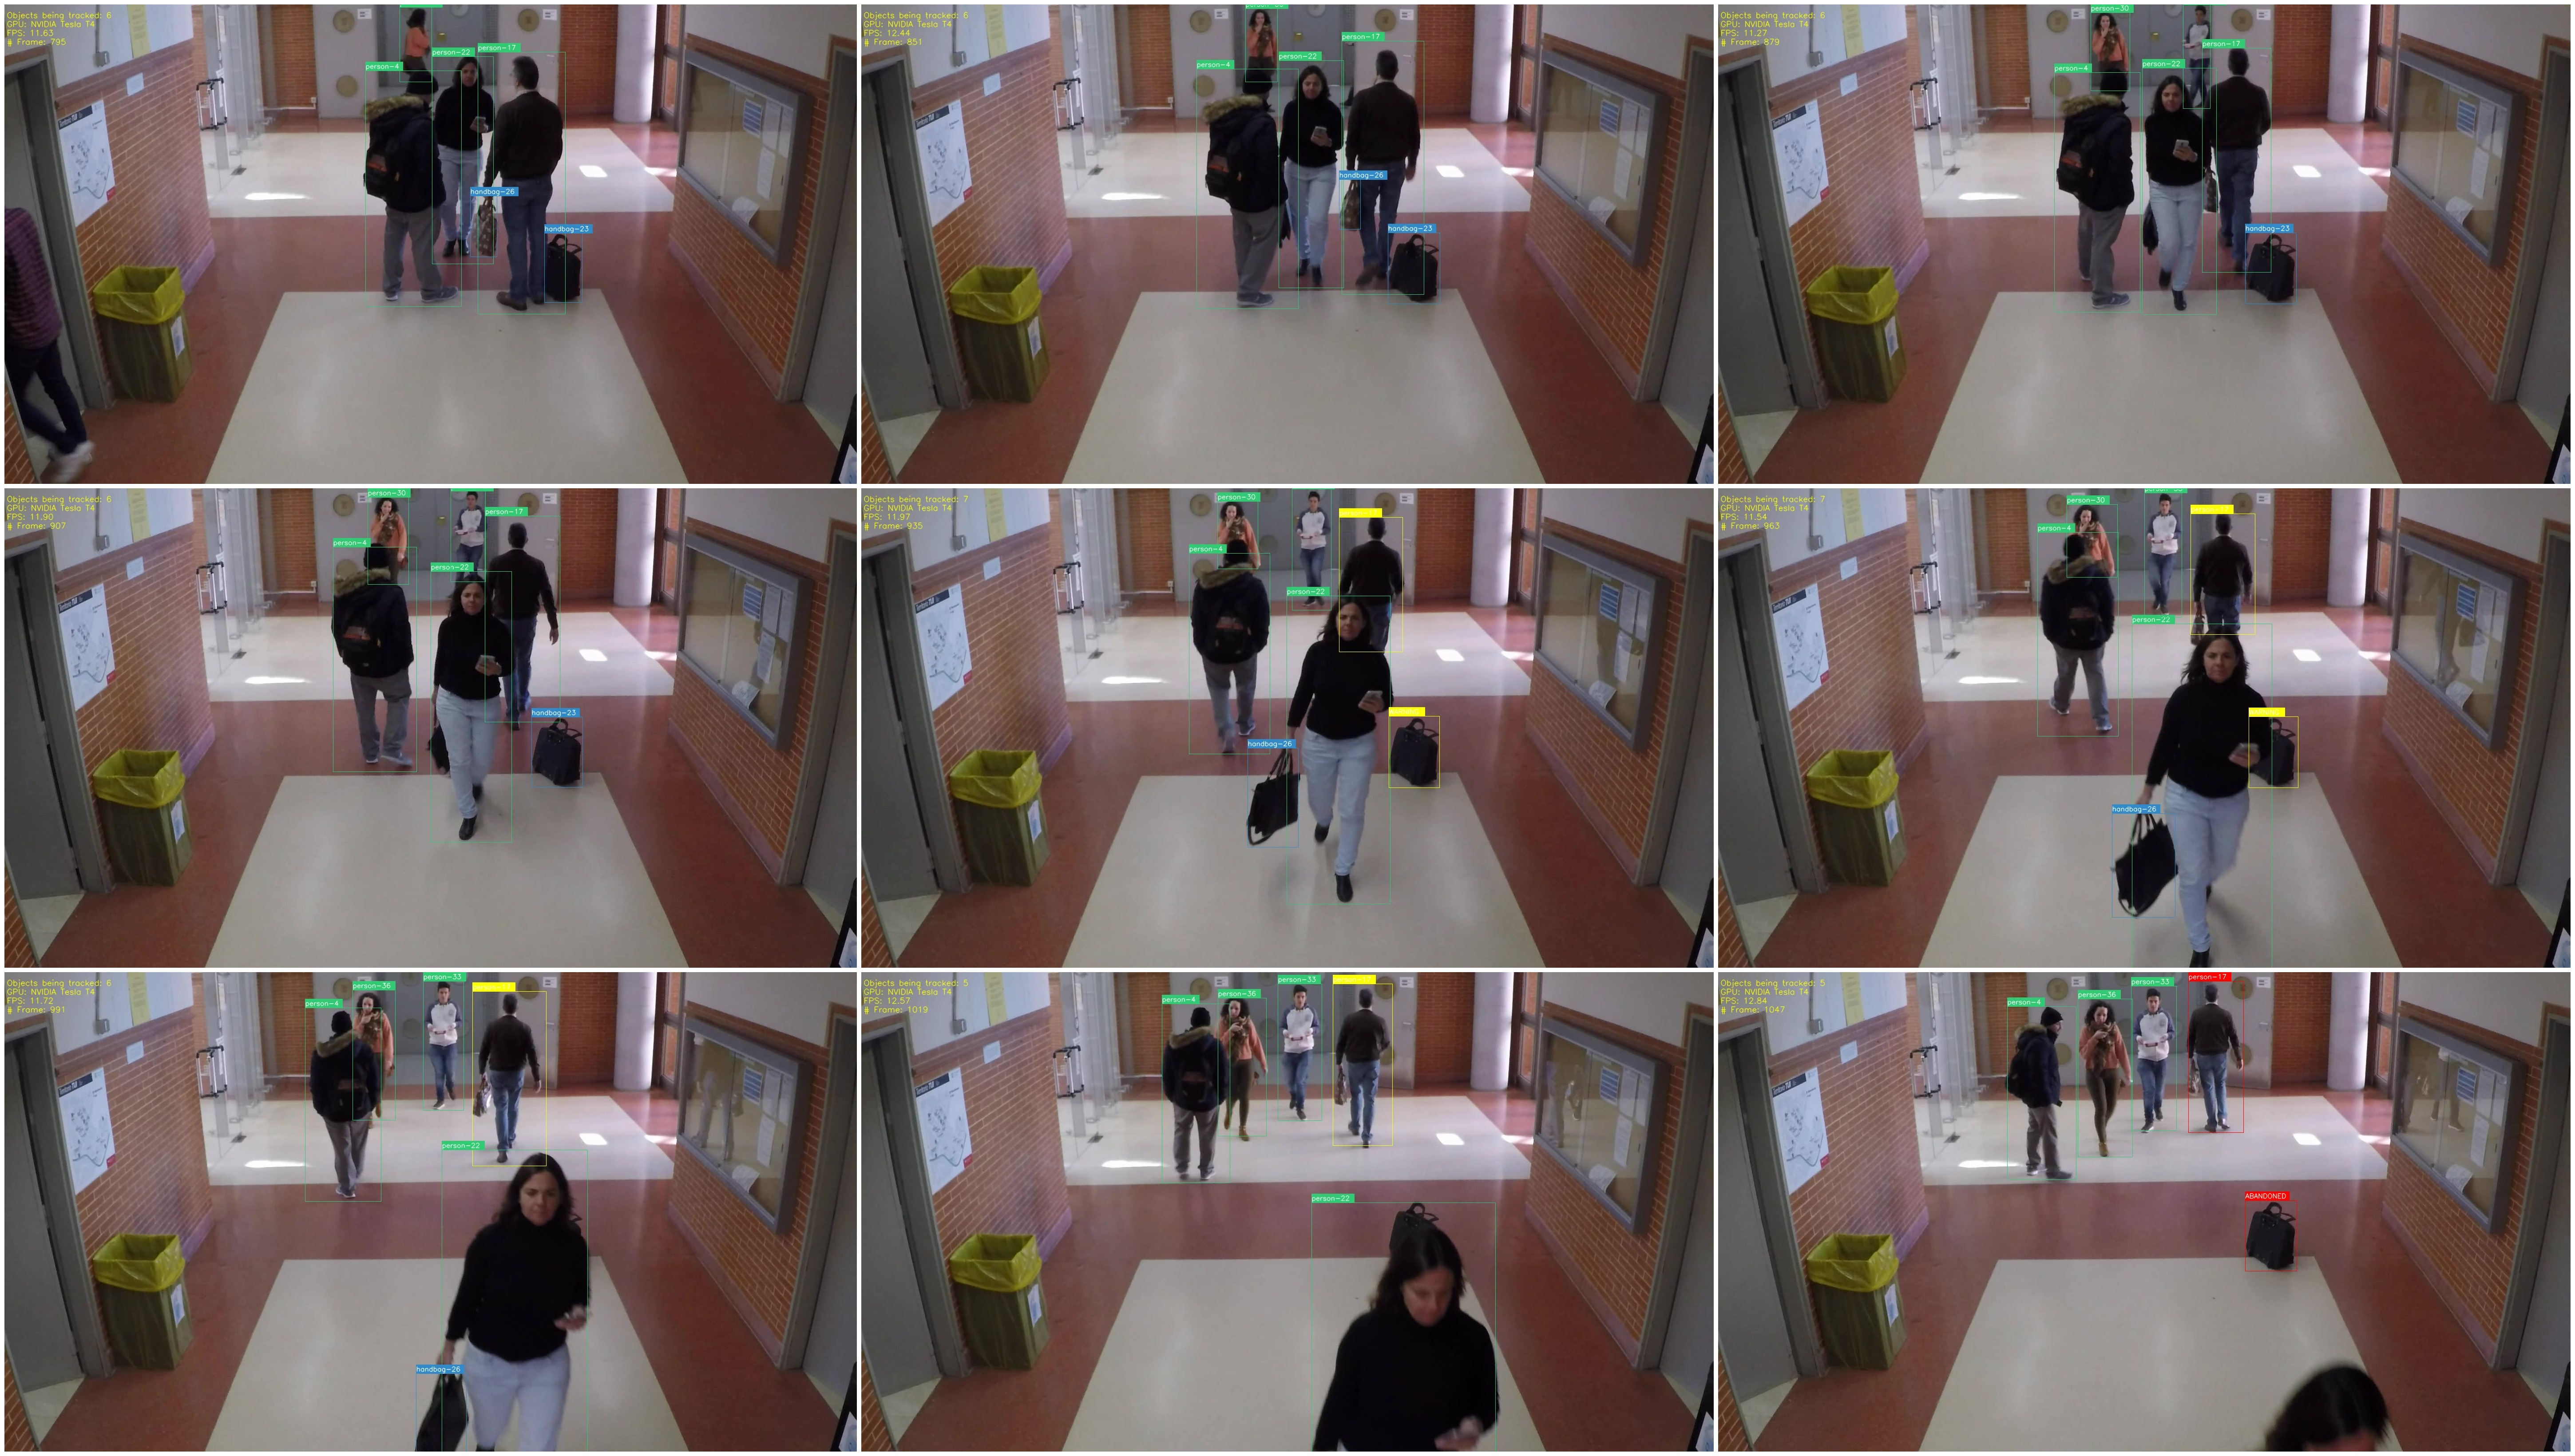
\includegraphics[width=0.85\textwidth]{img/chapters/resultados/abandono/1.png}
\caption{\label{fig:results1}Individuo abandona su bolsa de mano en el pasillo de cafetería de la EPS (1) \cite{gba-dataset}}
\end{figure}

En las figuras \ref{fig:results1} y \ref{fig:results2} se puede observar un claro ejemplo de uno de los problemas más comunes a la hora de detectar y rastrear objetos y personas, que se tratan de las oclusiones. Este fenómeno se produce cuando una persona u objeto se sitúa delante del otro, dificultando en la mayoría de ocasiones las detecciones y provocando cambios de identidad en el rastreo.

En la figura \ref{fig:results1} se puede observar como una persona con número de identidad 17 porta una bolsa de mano con número de identidad 23 y la posa sobre el suelo del pasillo de la entrada de la cafetería de la \gls{eps} \cite{gba-dataset}. También lleva otra bolsa de mano con número de identidad 26, pero no se detectó correctamente durante los primeros de segundos de vídeo y no se produjo la asociación. En cambio, con la bolsa de mano con identidad 23 sí. En los siguientes fotogramas se aprecia como la persona se aleja hacia el fondo del pasillo abandonando la bolsa de mano que dejó en el suelo anteriormente. De igual manera que en ejemplos anteriores, el algoritmo avisa cuando la bolsa de mano se encuentra en zona de alarma mediante cuadros delimitadores amarillos y cuando se considera que ha sido abandonada en rojo.

\begin{figure}[ht]
\centering
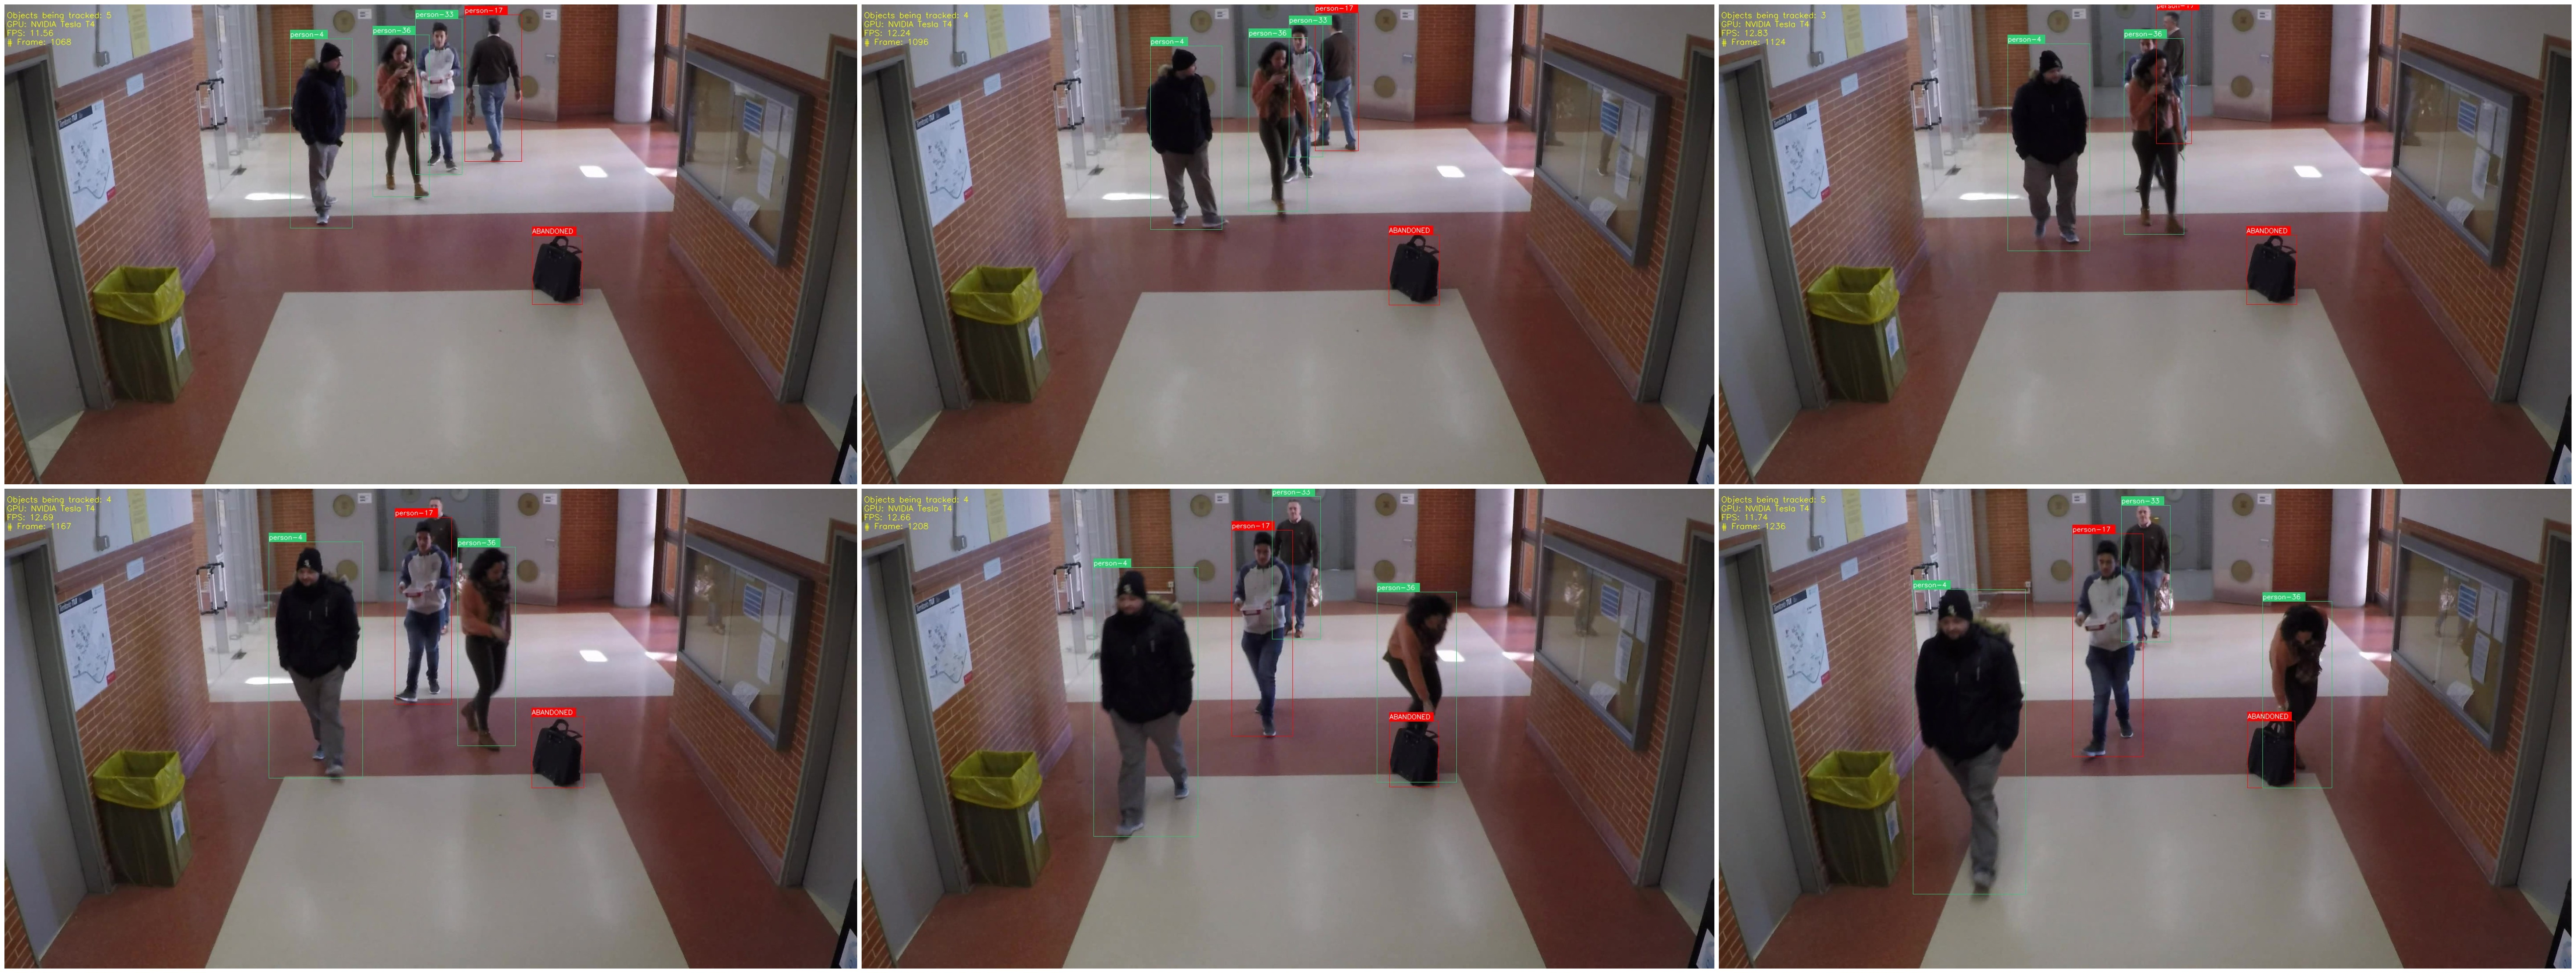
\includegraphics[width=0.85\textwidth]{img/chapters/resultados/abandono/2.png}
\caption{\label{fig:results2}Individuo abandona su bolsa de mano en el pasillo de cafetería de la EPS (2) \cite{gba-dataset}}
\end{figure}

En la figura \ref{fig:results2} anterior se puede apreciar que ocurre el fenómeno de oclusión. Cuando el individuo llega al final del pasillo y se da la vuelta queda por detrás de la persona con número de identidad 33 y ésta a su vez se encuentra detrás de la mujer con número de identidad 36. Durante estos breves instantes que se está produciendo oclusión debido a la posición de los sujetos se pierden las detecciones y en consecuencia el rastreo, produciéndose un cambio de identidad entre la persona con identidad 17 y la persona con identidad 33. Como se puede ver, las oclusiones provocan grandes problemas ya que pueden producir cambios de identidad sobre personas a las que ya se le había asignado un objeto de su propiedad, y en este caso, lo acababa de abandonar. De tal manera que se está identificando como identidad provocadora del abandono a la persona incorrecta.

\begin{figure}[ht]
\centering
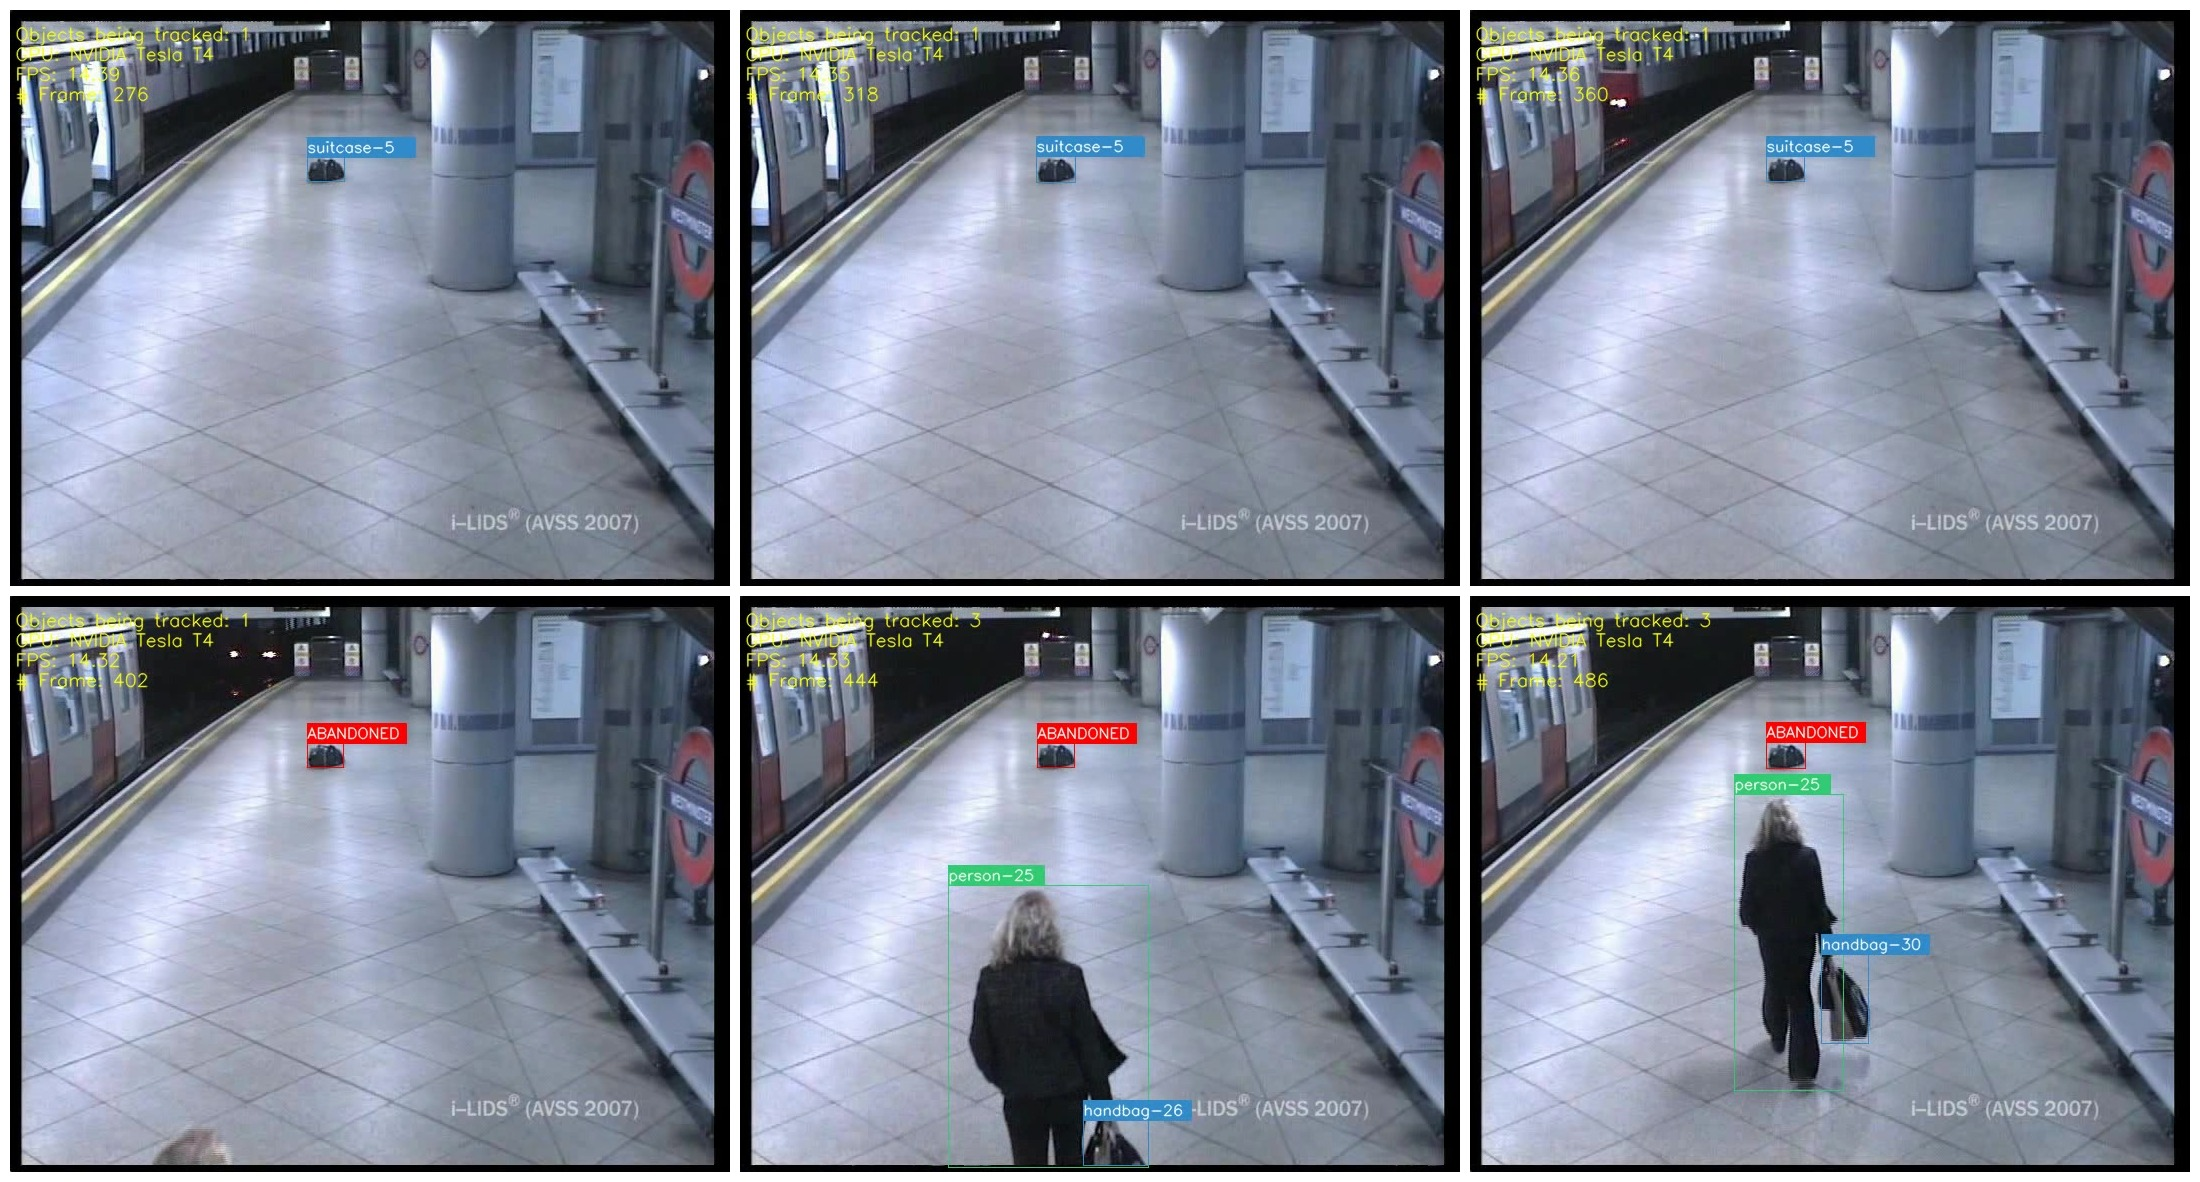
\includegraphics[width=0.85\textwidth]{img/chapters/resultados/abandono/3.png}
\caption{\label{fig:results3}Una bolsa de mano se encuentra abandonada al final de un andén de trenes \cite{AVSSAB2007-dataset}}
\end{figure}

Uno de los posibles escenarios que se barajó durante el desarrollo del algoritmo del detector de objetos abandonados en la sección \ref{sec:algoritmo-object-detection} es la posibilidad de que al inicio de una secuencia de vídeo se encontrara un objeto que no se le pudiera asignar como propietario a ninguna persona por que no se encontraba a la distancia mínima de asociación persona-objeto. En este fragmento de vídeo de una secuencia del dataset \gls{avss} \cite{AVSSAB2007-dataset} se puede observar como se detecta una bolsa de mano al final de andén que se encuentra desde un principio abandonado. En este caso, al tratarse de un vídeo de 25 \gls{fps}, si desde un primer momento el objeto está abandonado, al cabo de 15 segundos, es decir, 375 fotogramas después, el objeto se identifica como abandonado.

Como se puede observar en la primera imagen de la segunda fila de la figura \ref{fig:results3}, en el fotograma 402 ya se ha determinado esa bolsa de mano como abandonada. Cabe recalcar que, en objetos que se encuentran a una distancia alejada, en la etapa de detección suele confundir cuando es una maleta, una mochila o una bolsa de mano. En este caso está detectando la bolsa de mano como si fuera una maleta. 

En la figura \ref{fig:results4}, perteneciente a la evaluación del algoritmo de detección de objetos abandonados sobre un fragmento del dataset \gls{pets} \cite{pets2007-dataset}, se aprecia a una persona que inicialmente se le ha asignado como número de identidad el 28, porta una bolsa grande de deporte donde en un principio el algoritmo de detección lo confunde con una persona.

\begin{figure}[ht]
\centering
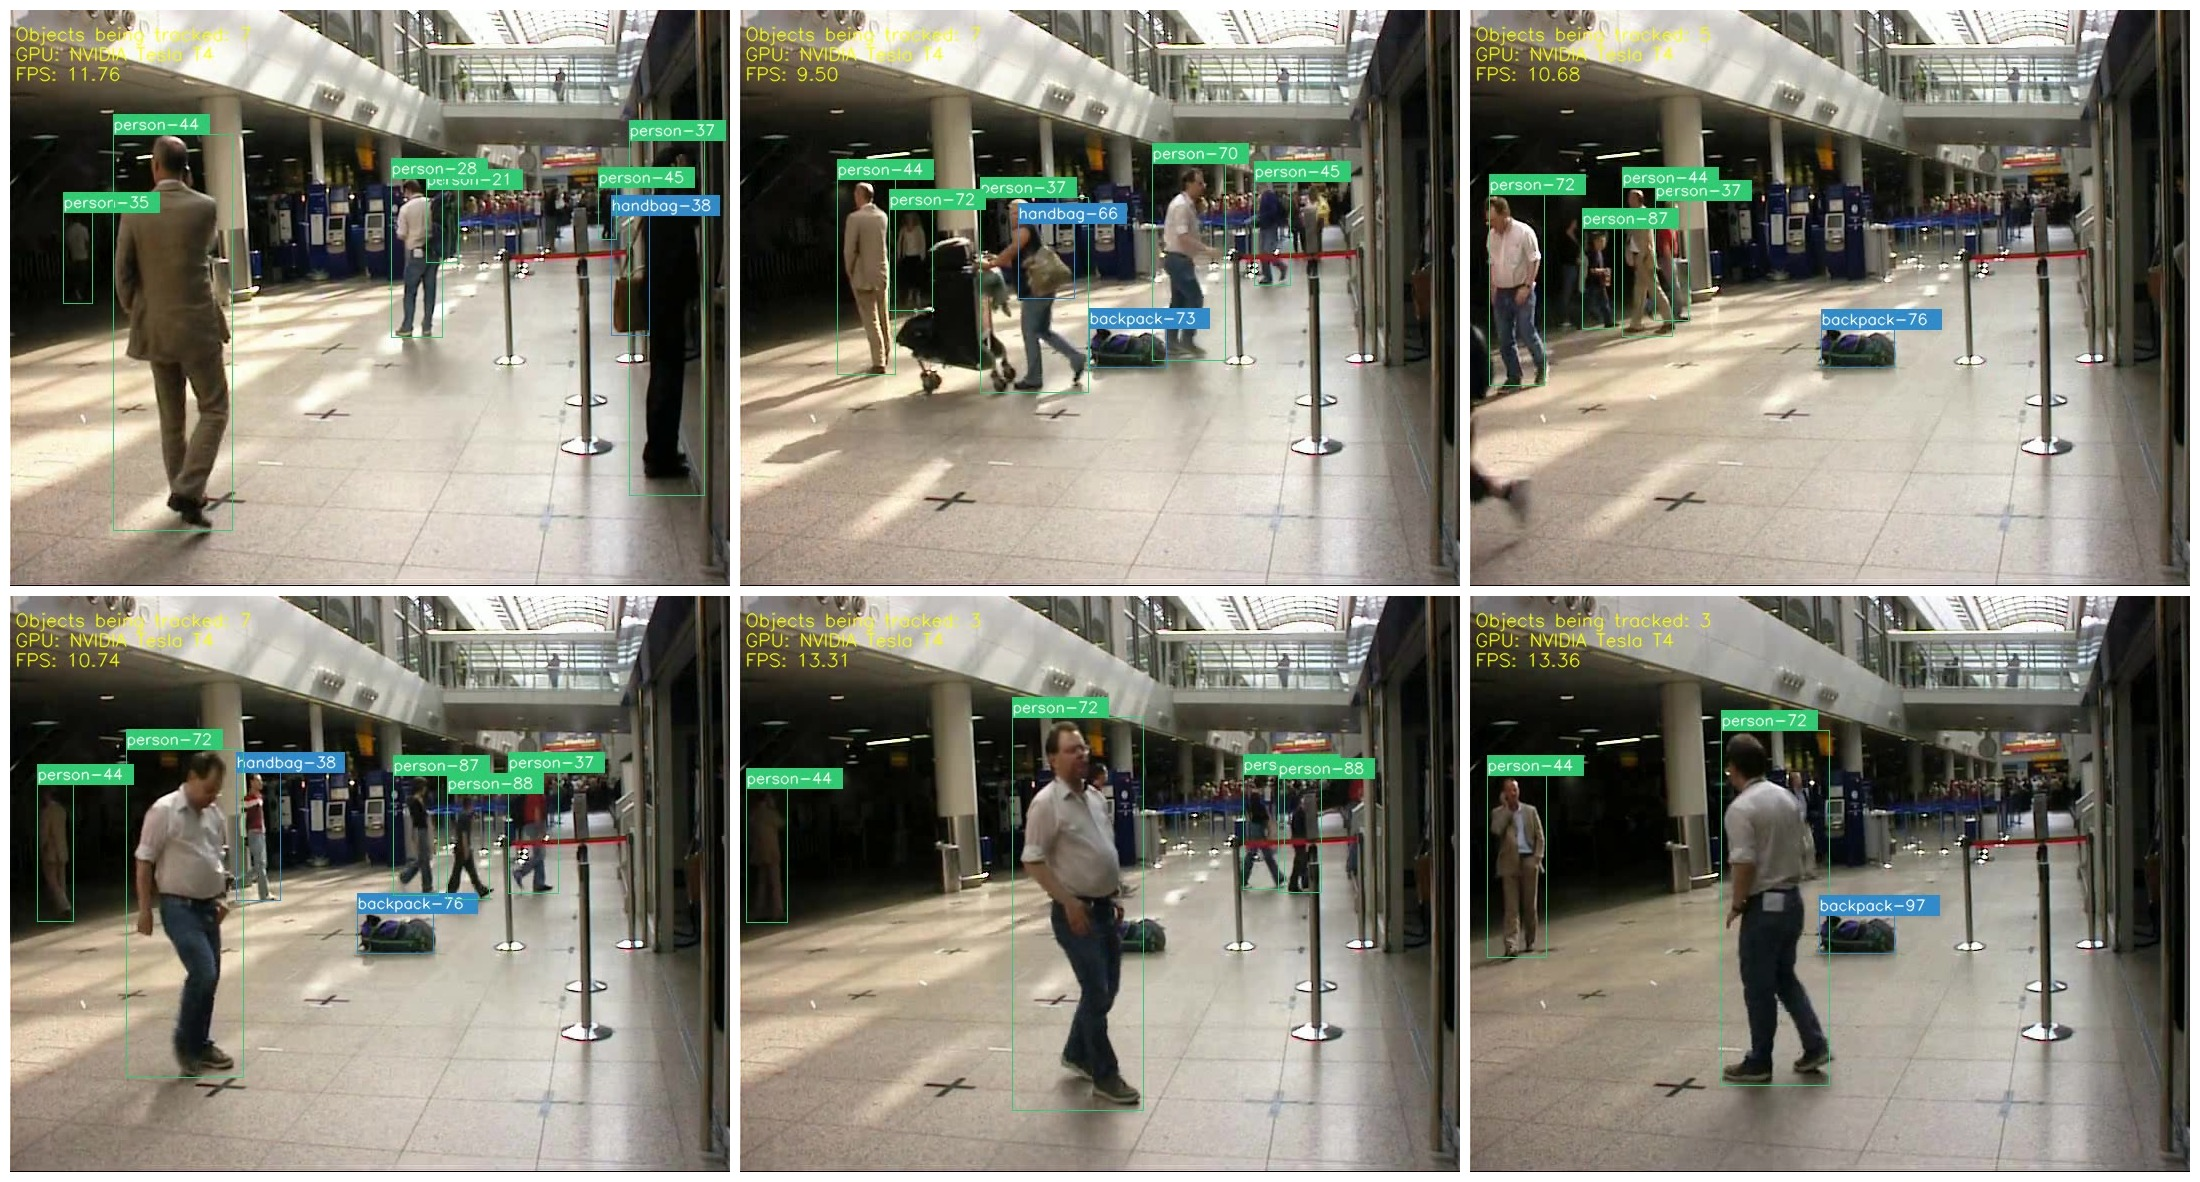
\includegraphics[width=0.85\textwidth]{img/chapters/resultados/abandono/4.png}
\caption{\label{fig:results4}Individuo abandona una bolsa de deporte en un aeropuerto \cite{pets2007-dataset}}
\end{figure}

En los siguientes fotogramas cambia la identidad de la persona al número 70 y ya se le ha asignado una identidad de objeto a la bolsa de deporte con la identidad 73 (ver segunda imagen de la primera fila de la figura \ref{fig:results4}). Pocos fotogramas después vuelven a cambiar las identidades tanto de la persona como de la bolsa de deporte a 72 y 76 respectivamente. En este punto ya se ha terminado el periodo de asignación de objetos a personas con lo cual no es posible crear una asociación, además en ese momento la persona se encuentra alejada de la bolsa desatendida. Cuando la persona vuelve a acercarse a la bolsa de la cual es propietario vuelve a ocurrir el fenómeno de oclusión que se vio en el ejemplo sobre el dataset \gls{gba2018} \cite{gba-dataset}. Al moverse, una vez más, vuelve a cambiar la identidad de la bolsa de deporte a 97. Todos estos sucesos de cambios de identidad que se producen en esta secuencia de vídeo son producidos por las oclusiones de las personas que se van moviendo por la zona del aeropuerto, imposibilitando la creación de asociación entre personas y objetos.

Como se ha podido observar en los ejemplos que se acaban de exponer, el algoritmo que se ha propuesto para el propósito de este proyecto funciona correctamente siempre y cuando se ejecuten las etapas de detección y rastreo de objetos y personas sin errores. El principal problema que se ha encontrado en esta parte del trabajo ha sido las oclusiones producidas, lo que conlleva a pérdidas de detecciones y en consecuencia a cambios de identidad o tener que volver que reidentificar, impidiendo la asociación persona-objeto o asignando como responsable de un abandono a la persona equivocada.

Todos los fotogramas han sido extraídos de las secuencias procesadas, las cuales se pueden acceder en el siguiente \href{https://drive.google.com/drive/folders/1AA4KZCpsEW6MTdHJdu8mLKuGE1BCX9de?usp=sharing}{link}.

\newpage % Para que no salte error por la imagen de arriba

\section{Conclusiones}
\label{sec:conclu-resultados}

Este capítulo se ha dividido en dos partes claramente diferenciadas. En la primera parte se han calculado las métricas de calidad sobre los dos datasets utilizados en este proyecto, \gls{coco} y \gls{oidv4}. En la segunda parte se han evaluado, primeramente \gls{yolov4}, seguido del algoritmo de rastreo \gls{deepsort} y por último, el algoritmo de detección de objetos abandonados que se desarrolló en la sección \ref{sec:algoritmo-object-detection} sobre los datasets más relevantes en la evaluación algoritmos de detección de objetos abandonados como pueden ser \gls{aboda} \cite{aboda-dataset}, \gls{gba2018} \cite{gba-dataset}, \gls{avss} \cite{AVSSAB2007-dataset} o \gls{pets} \cite{pets2007-dataset}.

Pese a que las métricas obtenidas en el dataset \gls{coco} sobre las clases de interés: \texttt{Person}, \texttt{Suitcase}, \texttt{Handbag} y \texttt{Backpack} son buenas, se pretendió intentar mejorarlas entrenando una \gls{cnn} basada en imágenes de las mismas clases del dataset \gls{oidv4}, ya que dispone de imágenes diferentes a las de \gls{coco}. Tras finalizar el primer entrenamiento, se pudo ver en las tablas \ref{tab:metricas-test1_4} y \ref{tab:comparativa-metricas2} que a pesar de que se obtuvieron buenos resultados de \gls{map}, los valores de precisión, Recall y F-score fueron inferiores a las de \gls{coco}.

Posteriormente, se volvió a intentar mejorar las métricas aumentando el número de clases de entrenamiento, ya que el dataset \gls{oidv4} dispone de más clases de interés como pueden ser \texttt{Plastic bag}, \texttt{Luggage and bags} y \texttt{Briefcase}. También, se aumentaron el número de imágenes de entrenamiento y validación así como el número de máximas iteraciones. Los resultados que se obtuvieron en las tablas \ref{tab:metricas-test2_2}  y \ref{tab:comparativa-metricas2} fueron similares a las del primer entrenamiento, por lo que se decidió continuar el proyecto utilizando el dataset \gls{coco} sobre el que viene pre-entrenado \gls{yolov4}.

En la segunda parte del presente capítulo se ha evaluado en primer lugar la etapa de detección con el funcionamiento de \gls{yolov4} sobre los distintos datasets antes nombrados. A pesar de que se mejoran las predicciones en términos de velocidad-precisión respecto a los resultados obtenidos en \cite{valdivieso2018}, siguen apareciendo el problema de las oclusiones. Cuando una persona se sitúa por delante del otra respecto al plano frontal de la cámara, fácilmente identifica únicamente a la persona que se encuentra más cerca, lo que conlleva que en la etapa de rastreo no se le pueda asignar una identidad a dicha persona. Lo mismo ocurre con los objetos de interés. Se ha observado que con una única red pre-entrenada no se detecta de la misma forma sobre los datasets evaluados. Como ya se vio en el último ejemplo de la sección \ref{subsec:resultados-yolov4-tf}, fenómenos como pueden ser los cambios de iluminación, calidad en la resolución del vídeo, escenas de día/noche, objetos de interés a largas distancias y en ángulos desfavorables u oclusiones, provocan que las predicciones se vean afectadas ocasionando en múltiples ocasiones \gls{fp}.

Posterior a la evaluación de la etapa de detección con \gls{yolov4} se ha analizado los resultados ejecutando el algoritmo de detección y seguimiento con \gls{deepsort}. Con el fin de que no se producieran \gls{fp} se aumentó el umbral de confianza de 0,25, valor que se ha utilizado por defecto en la evaluación de las predicciones en la detección con \gls{yolov4}, a un valor de 0,45. Con ello se ha asegurado un rastreo confiable en los objetos detectados en la etapa previa. Sin embargo, del mismo modo que cuando se evaluaron las detecciones, las clases \texttt{backpack} y \texttt{handbag} se confundían con frecuencia y con el transcurso de los fotogramas cambiaba la clase detectada y en consecuencia se perdía la identidad que se le había asignado a dicho objeto. Otro problema que se ha encontrado con frecuencia y que está totalmente vinculado a la etapa de detección es la aparición de oclusiones en secuencias de vídeo de grandes aglomeraciones de personas. Al pasar una persona por delante de otra desde el punto de vista frontal de la cámara podían ocurrir dos sucesos. El primero es que solo se detectara a una persona (la persona que se encontraba en el primer plano), con lo cual se perdía la detección y con ello el rastreo de la identidad de la persona que se encontraba en el segundo plano. El otro suceso se trata cuando dos personas se cruzaban y se producía un intercambio de identidad. En ambos casos perjudicaba el rastreo de objetos y personas, así como la asociación persona-objeto en el algoritmo de detección de objetos abandonados.

Finalmente, el algoritmo de detección de objetos abandonados que se planteó en la figura \ref{fig:abandoned-object-scheme} funciona correctamente, pero es totalmente dependiente de que la etapa de detección y la etapa de seguimiento de personas y objetos se realicen sin fallos. Aparecieron dos principales problemas durante la evaluación del algoritmo. Uno de ellos fueron las oclusiones producidas por las personas durante las secuencias de vídeo de grandes aglomeraciones, lo que provocaba cambios de identidad entre los sujetos y en consecuencia, incapacidad de establecer una asociación persona-objeto al inicio del vídeo. El segundo problema fue los cambios de clase, sobre todo en bolsa de mano pequeñas. En ciertas ocasiones, según el ángulo donde se situase el objeto, en la etapa de detección se realizaban predicciones de que el objeto era una mochila, y fotogramas después pasaba a ser una bolsa de mano. Esto producía que no se pudiera crear la asociación persona-objeto o que, una vez creada, desapareciese la identidad del objeto de la secuencia de vídeo.
